%! TEX program = xelatex
%!TEX encoding = UTF-8 Unicode

\documentclass[engineeringmaster]{hquThesis}
\titleZh{论文中文题目}
\titleEn{English Thesis Title}
\authorZh{吴新瑜}
\authorEn{}
\id{}
\schoolZh{土木工程学院}
\schoolEn{}
\supervisorZh{}
\supervisorEn{}
\cosupervisorZh{}
\fieldZh{}
\fieldEn{}
\major{}
\coverdate{二〇二三年五月二十八日}



\begin{document}
\makecover
\frontmatter
\begin{abstract}
无网格法是一类根据离散节点信息直接建立形函数的方法,其形函数具有高阶光滑的特点,适用于薄板等高阶问题。
本论文讨论的是具有变分一致性的伽辽金无网格法,目前具有变分一致性的伽辽金无网格法主要是通过假定应变理论构造匹配的光滑梯度,
再生光滑梯度理论框架为假定应变的光滑梯度提供了一个通用的表达式,并在伽辽金弱形式中直接将光滑梯度替换成传统无网格形函数梯度。
但光滑梯度并不等于传统无网格形函数梯度,该过程缺乏完备的变分原理理论基础。为了满足全域的变分一致性,满足积分约束条件的无网格数值积分方案需要配合具有变分一致性的本质边界条件施加方案,
现有的本质边界条件施加方法还存在诸多问题,亟待发展一种全新变分一致本质边界条件施加方案。\par
首先,基于Hellinger-Reissner变分原理推导余能泛函,分别对位移和应力变分可以得到Hellinger-Reissner原理弱形式。其中位移采用传统无网格形函数进行离散,而应力采用在每个积分域中假设为多项式,以满足局部的变分一致性。
随后,根据Hellinger-Reissner变分原理弱形式中内嵌本质边界条件的特点,以Hellinger-Reissner变分原理弱形式为基础系统推导本质边界条件施加过程中的离散控制方程。
此时的无网格离散方程可看作为一种新型的Nitsche法施加本质边界条件,其中修正变分项采用再生光滑梯度和无网格形函数进行混合离散,稳定项则内嵌于Hellinger-Reissner变分原理弱形式中,无需额外增加稳定项。
最后,详细分析该方法的变分一致性,并详细对比所提方法和传统Nitsche法、罚函数法、拉格朗日乘子法之间的差别,并通过传统弹性力学问题和薄板问题验证所提方法的计算精度和效率。
该方法消除了对人工参数的依赖性,也无需计算复杂耗时的形函数梯度,并满足积分约束条件,有效的提高计算精度和计算效率。
\par
\end{abstract}
\keywords{无网格法;Hellinger-Reissner变分原理;本质边界条件;再生光滑梯度;变分一致性}
\begin{abstractEn}
    hjrfjhfj\par
\end{abstractEn}
\keywordsEn{keyword1;keyword2;keyword3;keyword3}
\tableofcontents





\mainmatter
\chapter{绪论}
\section{引言}
由于实际工程中的结构通常具有复杂的几何形状、材料是非线性以及多样化的荷载情况,从而使得经典的解析方法难以直接应用于工程实际中进行计算和分析,需要借助数值计算分析方法进行求解。
有限元法\textsuperscript{\cite{hughes2000,2014Computer,steinEncyclopediaComputationalMechanics2018,2013Nonlinear}}是目前最常采用的数值分析方法,是通过将复杂的结构问题离散化为许多小的有限元单元,并在每个单元上建立近似的数学模型,进而将复杂的问题转化为求解一系列简化的局部问题。
这种离散化的方法使得有限元法能够有效地处理各种复杂的几何结构模型,材料和几何的不连续性以及不规则荷载,有限元法还可以通过划分网格数量,调整网格密度灵活地处理各种几何形状,进一步提高计算精度。
虽然有限元法是一种广泛应用于解决复杂工程问题的数值方法,但有限元的计算结果在很大程度上依赖于网格的划分。对于复杂的薄板几何形状,需要细致划分网格才能获得准确的解,网格密度增加会引起计算增加, 降低计算效率,并且用有限元法处理薄板的剪切变形存在一定的困难,会导致数值计算结果有一定的误差。
值得注意的是,基于单元插值的有限元法通常只有$C^0$联系,难以构造整体协调的$C^1$单元,无法直接求解要求$C^1$是连续的薄板等高阶问题。
\par
无网格法\textsuperscript{\cite{chenMeshfreeMethodsProgress2017,belytschkoMeshlessMethodsOverview1996b}}是一类能够有效解决高阶薄板问题的数值分析方法,
该方法是一类根据离散节点位置信息直接建立形函数的方法,其形函数具有高阶光滑的特点,不依赖于网格单元信息构造形函数,有效的避免了网格划分,网格畸变等问题,使得无网格法在处理薄板问题中的几何变化具有更好的适应性,稳定性和可靠性。无网格法可以直接考虑薄板的厚度变化,能够准确地捕捉薄板的弯曲和扭转行为。
根据无网格形函数构造不依赖于网格的特点,该方法也是用其他复杂的几何结构模型的离散,
如大变形分析\textsuperscript{\cite{陈嵩涛2020几何非线性分析的高效高阶无网格法}}、裂纹扩展模拟\textsuperscript{\cite{GaoXin2018}}以及薄板等高阶问题\textsuperscript{\cite{邓立克2019薄板分析的线性基梯度光滑伽辽金无网格法}},有效的提高因为网格划分因素所引起的计算精度下降的问题。
\section{伽辽金无网格法研究历史及现状}
上个世纪七十年代,由Lucy\textsuperscript{\cite{1977A}}、Gingold和Monaghan\textsuperscript{\cite{gingold1977}}提出的光滑水动力学法(SPH,Smoothed Particle Hydrodynamics)开启了众多学者对无网格法的关注,该方法是采用核函数的近似方法通过对求解域进行离散化,并使用强形式进行数值求解的近似方法,该方法属于配点型无网格法。
该方法具有构造简单,无需数值积分等优势被广泛应用于进行数值计算分析,但由于配点型无网格法是通过核近似的离散方式一般不满足一致性条件,使得该方法无法准确的保证数值计算的稳定性及计算精度\textsuperscript{\cite{auricchio2010a,wang2018a,wang2020,gomez2016}}。
% \par
1992年Nayroles等人\textsuperscript{\cite{nayroles1992}}使用移动最小二乘近似形函数并通过伽辽金弱形式提出了散射元法。
1994年Belytschko等人\textsuperscript{\cite{belytschko1994}}指出了散射近似(Scattered Data Approximation)实质上等同于移动最小二乘近似(Moving Least Squares, MLS)。通过对移动最小二乘近似函数进行精确求导,引入背景网格和高阶高斯积分方法改善数值积分的精度,通过引入拉格朗日乘子,可以在伽辽金无单元法中有效地施加边界条件,从而提高计算精度和稳定性。在这些改进的基础上,Belytschko等人将方法命名为伽辽金无单元法(Element Free Galerkin Method, EFG)。
值得注意的是,在采用伽辽金法进行求解的时候,由于无网格形函数一般不是多项式,计算时需要采用建立高阶高斯积分法或其他数值积分方法\textsuperscript{\cite{de2001,carpinteri2002,WangBingBing2019}},从而会导致计算效率降低\textsuperscript{\cite{melenk1996,WuJunChao}}。为了提高伽辽金无网格法的计算效率,众多学者进行了相关研究工作致力于解决伽辽金无网格法在计算过程中的效率问题\textsuperscript{\cite{wang2016,wang2019,chen2001,chen2013,duan2012,duan2014}}。
% \par
1995年Liu等人\textsuperscript{\cite{liu1995}}在光滑水动力学(Smoothed Particle Hydrodynamics, SPH)核近似方法的基础上进行了改进。他们引入了核近似的多项式再生条件和校正函数,提出了再生核近似(Reproducing Kernel Approximation, RK)和再生核质点法(Reproducing Kernel Particle Method, RKPM)。
1997年Babuška和Melenk\textsuperscript{\cite{melenk1996,babuska1997}}将系数矩阵表示为单位矩阵加上一个低秩矩阵的形式,使得原始线性方程组表示为多个规模较小的子问题的组合,每个子问题可以被独立的求解,进而求解出整个方程组的解,该方法称为单位分解法(PUM, Partition of unity method)也称为广义有限元法\textsuperscript{\cite{strouboulis2001}}。
1998年Sukumar等人\textsuperscript{\cite{sukumar1998}}提出了自然单元法,该方法通过将计算域划分为多个自然单元来离散化问题,通过使用自然领域形函数来近似解,并通过插值技术在整个计算域中进行扩展,该方法的形函数只具有$C^0$连续性,难以求解高阶薄板问题。
为了更好利用无网格法求解薄板问题,
2002年Long S等人\textsuperscript{\cite{long2002}}利用局部加权函数构建近似函数,并在控制方程中使用高斯积分法进行数值积分提出伽辽金局部无网格法(Meshless Local Petrov–Galerkin)。
2006年Liu等人\textsuperscript{\cite{liu2006}}利用径向基函数构建近似函数,并使用Hermite插值获得薄板的位移和旋转的连续性提出了Hermite径向点插值(Hermite Radial Point Interpolation)。
2011年Mill´an D等人\textsuperscript{\cite{millan2011}}利用最大熵原理构建一个最大熵函数,通过最大化信息熵确定最优的近似解提出了最大熵无网格法(Maximum-entropy Meshfree  Method ),通过这种方式从散点数据中生成连续的薄壳几何形状和应力场。
2012年Oh H等人\textsuperscript{\cite{oh2012}}通过将薄板离散为一组粒子,并利用粒子间的相互作用进行计算提出了单元划分方法。
随后2015年Chen等人\textsuperscript{\cite{chen2015}}提出了复变量(complex variable RKPM )方法,该方法基于粒子离散化,通过复变再生核函数近似求解数值分析。
2016年Thai等人\textsuperscript{\cite{thai2016}}利用移动Kriging插值构建近似函数,使用细化板理论进行描述薄板的受力状态提出了移动Kriging无网格法( Moving Kriging Meshfree Method),进而直接计算出薄板的位移和应力场。
不久,王东东,王莉华等人\textsuperscript{\cite{wang2020,wang2021}}提出了一种无网格配置方法该方法利用梯度再生核函数进行构建近似函数,并通过引入梯度项提高数值计算的稳定性和精度,可以准确得计算薄弹性梁和薄板的位移和应力分析,并进行相应的静态和动态分析。
为了更好的利用无网格法解决不同类型的问题,现如今已经提出了各式各样的无网格方法\textsuperscript{\cite{ChengYuMin2005,TanXianYun2011,LianYanPing2013,ZhangXiong2017,GaoXiaoWei2019}},关于更多目前无网格法的研究进展见文献\textsuperscript{\cite{nguyen2008,liu2009,张雄2009无网格法的理论及应用,wang2014,yreux2017,koester2019,rohit2018,王莉华2021配点型无网格法理论和研究进展,LiuYuXiang2021,朱志辉2021基于,sriram2021,ChenJian2022,LiYuDong2022}}
\par
本论文讨论的是具有变分一致性的伽辽金无网格法\textsuperscript{\cite{babuska2008,wu2021}}。
无网格形函数及其梯度通常为有理式,并且形函数的影响域具有高度重叠的特点导致无网格形函数在背景积分单元上为分段的有理式。
在伽辽金法的求解过程中,传统基于多项式完备性建立的高斯积分法无法进行准确数值积分过程,导数伽辽金无网格法无法准确求解与其基函数阶次相同的解析解,即不满足变分一致性\textsuperscript{\cite{1999Numerical}}。
为了解决该问题,建立具有变分一致性的伽辽金无网格法成为无网格研究领域的热门问题。目前具有变分一致性的伽辽金无网格发主要是通过假定应变理论构造匹配的光滑梯度,光滑梯度为低阶多项式,采用低阶高斯积分法既能准确进行数值积分,保证计算误差的收敛性。
同时,光滑梯度的构造过程仅需要计算传统无网格形函数,避免复杂耗时的形函数梯度计算,提高传统伽辽金无网格法的计算效率。
为了满足积分约束条件,Chen等人从伽辽金法的线性准确性条件出发,提出了线性积分约束条件\textsuperscript{\cite{chen2001}}。
段庆林等人\textsuperscript{\cite{陈嵩涛2020几何非线性分析的高效高阶无网格法,duan2012}}将线性积分约束条件推广至高阶情况,并通过高阶积分约束条件计算高斯点处光滑梯度值,使得传统高斯积分法满足变分一致性,该方法称为一致性无单元伽辽金法。
王东东和吴俊超提出了再生光滑梯度理论框架\textsuperscript{\cite{wang2019}},该框架具有与传统无网格形函数相类似的表达式,光滑梯度构造过程中可重新合理优化数值积分点采样点位置和权重,减少无网格形函数的计算量,提高计算效率。
Wang和Ren\textsuperscript{\cite{wang2023}}提出了一致投影积分法,以投影形函数为基础建立替代传统形函数空间,通过将投影形函数代入原始无网格形函数中近似计算伽辽金弱形式,利用具有高阶高斯正交规则的相应阶三角形有限元形函数,进而满足任意阶积分约束条件。\par
除了以假定应变理论为基础的变分一致型无网格法外,Chen等人\textsuperscript{\cite{chen1996}}提出了修正变分积分法,该方法通过对基函数的变分导数进行近似,并在积分过程中考虑变分一致性,通过选择适当的积分点和积分权重,从而实现任意阶数的数值积分该方法能够准确的模拟大变形问题、非线性问题和冲击破坏问题,提高伽辽金无网格法中数值积分的准确性和一致性,保证数值计算精度提高计算效率。
但使用伽辽金无网格法求解偏微分方程通常会使用试函数和权函数进行构建离散形式的方程,在伽辽金无网格法中,试函数和权函数通常属于相同的函数空间,从而确保离散形式的刚度矩阵是对称的,而修正变分积分法中修正后的权函数和试函数不属于同一空间,导数刚度矩阵的非对称性,非刚度矩阵会引起数值解的误差,无法保证数值求解的稳定性和精确性。
王东东和吴俊超提出了嵌套子域积分法\textsuperscript{\cite{wang2016}},该方法利用子域划分和梯度平滑技术提高数值积分的准确性,通过将计算域划分为多个子域,并在每个子域内采用光滑应变,利用两层次积分域得到的刚度矩阵进行合理组合,消除二阶误差项进而满足二次变分一致性,但嵌套子域积分法中,确保各层次的嵌套子域完全相似是构造光滑梯度的一个要求,这意味着每个子域在几何形状或大小上都与其他子域完全相同,使得该方法难以推广至三维及高阶情况。
\par
与传统有限元法相比,无网格方法具有高阶连续光滑的特点。然而,这种连续性导致无网格形函数在离散节点上通常不具有插值性,这在求解过程中使得施加本质边界条件变得困难。
为了克服这个问题,许多学者提出了各种具有插值性的无网格近似方法,以便能够直接施加本质边界条件\textsuperscript{\cite{CaoYang2020,fernandez-mendez2004}},如奇异权函数法\textsuperscript{\cite{kaljevic1997}}、插值最小二乘法\textsuperscript{\cite{liu2019,ChenXinXin2021}}、复变量移动最小二乘法\textsuperscript{\cite{ChengYuMin2005}}、广义移动最小二乘法\textsuperscript{\cite{HuangJuan2007}}、变换法\textsuperscript{\cite{chen2000}}等。
然而,这类方法不是建立在变分原理基础上,无法保证节点之间位移边界条件施加精度和无网格法的变分一致性。
对于满足积分约束条件的无网格数值积分方法,如稳定节点积分法\textsuperscript{\cite{chen2001}}、一致性积分法\textsuperscript{\cite{陈嵩涛2020几何非线性分析的高效高阶无网格法,duan2012}}、变分一致积分法\textsuperscript{\cite{chen2013}}、嵌套子域积分法\textsuperscript{\cite{wang2016}}、再生光滑梯度积分法\textsuperscript{\cite{wang2019}}等,在计算过程中采用形函数的光滑梯度替换传统无网格形函数导数,在保证无网格法的计算精度核最优误差收敛率的同时提高了计算效率,但其本质边界条件仍需要具有具有变分一致性的方法进行施加\textsuperscript{\cite{WuJunChao,hillman2021}}。
\section{本文选题背景}
变分一致型伽辽金无网格法可追溯到2004年Chen等人\textsuperscript{\cite{chen2001}}提出的稳定节点积分法,该方法从伽辽金法的线性准确性条件出发,提出了线性积分条件。伽辽金数值积分方法需要从满足积分约束条件,才能秋娥及线性问题,即满足线性的变分一致性。该方法通过在节点周围引入额外的稳定项,改善对梯度突变和奇点的逼近,通过修改形函数和积分权重,构造一种稳定的节点积分方案,节点处的积分权重与节点处的梯度信息相关联,假设光滑梯度为常数,通过满足线性积分约束条件建立光滑梯度实现对数值解的稳定性。尽管稳定节点积分法在提高数值解稳定性和准确性具有一定的优势,但稳定节点积分法需要在节点周围引入额外的稳定项,会降低计算效率,并且额外稳定项的效果很大程度上依赖于参数的选择,选择不当的参数可能会引起数值解的不稳定性。
% \par
段庆林等人\textsuperscript{\cite{陈嵩涛2020几何非线性分析的高效高阶无网格法,duan2012}}将线性积分约束条件推广至高阶情况,通过对无网格方法中的形函数进行修正和优化,通过与修正的形函数结合实现对积分的二阶精确性。通过使用高阶RBF函数计算高斯积分点处光滑梯度值,使得传统高斯积分法满足变分一致性,提高几何非线性分析的计算精度和效率。但该一致性积分法在计算过程中选取的高斯点数需要与积分约束条件数保持一致,这导致在处理高阶问题时会降低计算效率。并且一致性积分法无法完全消除数值误差,数值误差在计算高阶导数的过程中会逐渐积累和传播,可能会降低计算精度。
% \par
王东东和吴俊超提出了再生光滑梯度理论框架\textsuperscript{\cite{wang2019}},该框架具有与传统无网格形函数相类似的表达式,统一了以假定应变为基础的变分一致型光滑梯度构造方案。在该理论框架下,光滑梯度构造过程可重新合理优化数值积分采样点位置和权重,从而减少无网格形函数的计算量,提高计算效率。
\textbf{目前,再生光滑梯度理论框架为假定应变的光滑梯度提供了一个通用的表达式,并在伽辽金弱形式中直接将光滑梯度替换成传统无网格形函数梯度。但该光滑梯度并不直接等于传统无网格形函数梯度,该过程缺乏完备的变分原理理论基础}。
\par
为了满足全域的变分一致性,满足积分约束条件的无网格数值积分方案需要配合具有变分一致性的本质边界条件施加方案,传统无网格形函数在自身节点处不具有插值性,Belytschko等人\textsuperscript{\cite{belytschko1994}}最早采用拉格朗日乘子法施加本质边界条件,该方法需要引入额外自由度离散拉格朗日乘子,当采用变分一致型无网格数值积分方案时,拉格朗日乘子的自由度需要和光滑梯度构造过程中积分点的位置保持一致,以满足变分一致性。采用过多自由度离散拉格朗日乘子将导致整体刚度矩阵出现奇异,以致于该方法不适合高阶的变分一致型伽辽金无网格法。
罚函数法\textsuperscript{\cite{zhu1998}}施加本质边界条件无需额外增加自由度,数值实现简单。广泛应用于伽辽金无网格法。但该方法的计算误差依赖于人工经验参数,且不具有变分一致性,不能保证计算精度。
Nitshce法\textsuperscript{\cite{fernandez-mendez2004}}是目前变分一致型无网格法主要采用的本质边界条件施加方法,该方法在修正变分原理的基础上引入罚函数法作为保证刚度矩阵的正定性。但是在积分一致的数值积分方案中已经不需要的无网格高阶梯度被重新引入,降低了无网格分析的计算效率。同时,Nitsche法中的稳定性还是需要人工经验参数,过大或过小的人工参数都将导致计算精度的降低。
另一类无网格施加本质边界条件的方法是试图恢复无网格形函数的插值性。Fernández-Méndez与Huerta\textsuperscript{\cite{fernandez-mendez2004}}通过修改无网格形函数构造过程中核函数的权重,使得无网格形函数在边界处具有插值性,但该方法无法满足积分约束条件。Hillman和Lin\textsuperscript{\cite{hillman2021}}在修正变分法中引入具有插值性无网格近似,但该方法改变了解的空间。Chen等人\textsuperscript{\cite{chen1996}}采用转换矩阵,将无网格法中的节点系数重新与物理值建立联系,从而直接施加本质边界条件,并称该方法为变换法。王东东\textsuperscript{\cite{wang2015}}将变换法引入稳定节点积分法中,并对其进行了修正,以保证数值积分的一致性。然而,变换法中转换矩阵需作用于整体刚度矩阵,计算量大,不适用于大规模计算。
\textbf{Nitsche法作为最适合变分一致型伽辽金无网格法的本质边界条件施加方法还存在诸多问题,如人工参数的依赖性,需要计算复杂耗时的形函数高阶梯度等,亟待发展一种全新变分一致型本质边界条件施加方案}。
\section{本文主要内容}
论文研究将发展基于Hellinger-Reissner原理的变分一致型伽辽金无网格法,优化该方法背景积分域的划分过程,并依托于Hellinger-Reissner原理内嵌本质边界条件的特点,建立具有变分一致性且不依赖于人工经验参数的本质边界条件施加方法,具体内容如下:\par
(1)\textbf{通过Hellinger-Reissner变分原理完善变分一致型伽辽金无网格数值积分方法的基础理论框架}。首先,基于Hellinger-Reissner(HR)变分原理推导余能泛函,分别对位移和应力变分可以得到HR原理弱形式。其中位移采用传统无网格形函数进行离散,而应力采用在每个积分域中假设为多项式,以满足局部的变分一致性。最后,通过分片实验和典型弹性力学问题验证该方法的变分一致性,精度和误差收敛性;\par
(2)\textbf{以Hellinger-Reissner原理为基础建立具有变分一致性且不依赖人工参数的本质边界条件施加方法}。首先,HR变分原理弱形式中内嵌本质边界条件,以HR变分原理弱形式为基础系统推导本质边界条件施加过程中的离散控制方程。详细分析该方法的变分一致性。并详细对比所提方法和传统Nitsche法,罚函数法,拉格朗日乘子法之间的差别,并通过传统弹性力学问题和薄板问题验证所提方法的计算精度和效率。




\chapter{无网格近似理论}
本章以再生核无网格法为例对伽辽金无网格法进行介绍,详细说明无网格形函数及其导数的构造过程,讨论无网格形函数的插值性。同时,介绍伽辽金无网格法在弹性力学问题和薄板问题上的应用。
\section{再生核无网格近似}
如图(\ref{nomeshpoint})所示的问题为例,无网格近似将求解域$\Omega$及其边界$\Gamma$离散为一系列无网格节点$\{\pmb{x}_I\}^{N\!P}_{I=1}$,
$N\!P$表示无网格节点数量。每个无网格节点$\pmb{x}_I$对应的形函数为$\Psi_I(\pmb{x})$,形函数影响域为$supp(\pmb{x}_I)$,
并要求影响域的覆盖域需包含求解域$\Omega$,即$\Omega\subseteq^{N\!P}_{I=1}supp(\pmb{x}_I)$。
考虑求解域$\Omega$内的一个变量$u(\pmb{x})$,其对应的无网格近似函数$u^h(\pmb{x})$可表示为:
\begin{equation}\label{ui}
\begin{split}
    u^h(\pmb{x})=\sum_{I=1}^{N\!P}\Psi_I(\pmb{x})d_{I}
\end{split}
\end{equation}
其中$d_{I}$表示与无网格节点$\pmb{x}_I$对应的节点系数。\par
\begin{figure}[H]
\centering
    
\includegraphics[scale=0.6]{Figure/nomesh/point.png}
    \caption{无网格离散示意图}\label{nomeshpoint}
\end{figure}\par
根据再生核近似理论\textsuperscript{\cite{liuReproducingKernelParticle1995}},无网格形函数可以假设为如下再生核形式:
\begin{equation}\label{shapefunction}
        \Psi_I(\pmb{x})=\sum_{I=1}^{N\!P}\pmb{p}^{[p]T}(\pmb{x}_I-\pmb{x})\pmb{c}(\pmb{x})\phi_s(\pmb{x}_I-\pmb{x})
\end{equation}
其中$\pmb{p}^{[p]}(\pmb{x})$为$p$阶的多项式基函数向量,其表达式为:
\begin{equation}
    \pmb{p}^{[p]}(\pmb{x})=\{1,\;x,\;y,\;\dotsb,\;x^iy^i,\;\dotsb,\;y^p\},\quad 0\le i+j \le p
\end{equation}
而$\phi_s(\pmb{x}_I-\pmb{x})$为附属于节点$\pmb{x}_I$的核函数,其影响域的大小由影响域尺寸$s$决定,核函数及其影响域的大小共同决定了无网格形函数的局部紧支性和光滑性。在二维情况下,核函数$\phi_s(\pmb{x}_I-\pmb{x})$的影响域通常为圆形域或者矩形域[]。本文的影响域形状均为矩形,矩形影响域的核函数可由下列公式计算得到:
\begin{equation}
    \phi_s(\pmb{x}_I-\pmb{x})=\varphi(r_x)\varphi(r_y),\quad r_x=\frac{\lvert x_I-x\rvert}{s_x},r_y=\frac{\lvert y_I-y \rvert}{s_y}
\end{equation}
其中$s_x$和$s_y$分别为$x$和$y$方向上影响域尺寸的大小,在均匀布置的节点下,计算时一般使得两个方向上的影响域大小相等即$s_x=s_y=s$。为保证紧支性和光滑性,$\varphi$通常取为阶次大于$p$的紧支函数。本文针对弹性力学问题,无网格基函数一般选择二阶或者三阶多项式基函数,核函数$\phi_s(\pmb{x}_I-\pmb{x})$取为三次样条函数:
\begin{equation}
    \varphi(r)=\frac{1}{3!}
\begin{cases}
    (2-2r)^3-4(1-2r)^3 &r\le \frac{1}{2}\\
    (2-2r)^3&\frac{1}{2}<r\le 1\\
    0&r>1
\end{cases}
\end{equation}\par
针对薄板和薄壳问题,无网格基函数一般选择三阶或四阶多项式基函数,核函数$\phi_s(\pmb{x}_I-\pmb{x})$取为五次样条函数:
\begin{equation}
        \varphi(r)=\frac{1}{5!}
\begin{cases}
        (3-3r)^5-6(2-3r)^5+15(1-3r)^5&r\le\frac{1}{3}\\
        (3-3r)^5-6(2-3r)^5&\frac{1}{3}<r\le\frac{2}{3}\\
        (3-3r)^5&\frac{2}{3}<r\le1\\
        0&r>1
\end{cases}
\end{equation}\par
最后,无网格形函数表达式(\ref{shapefunction})中$\pmb{c}$为待定系数向量,该待定系数通过满足下列一致性条件[]确定:
\begin{equation}\label{regeneration conditions}
    \sum_{I=1}^{N\!P}\Psi_I(\pmb{x})\pmb{p}(\pmb{x}_I-\pmb{x})=\pmb{0}
\end{equation}
将式(\ref{shapefunction})代入到式(\ref{regeneration conditions})中即可得到待定系数向量$\pmb{c}(\pmb{x})$的具体表达式:
\begin{equation}\label{c}
    \pmb{c}(\pmb{x})=\pmb{A}^{-1}(\pmb{x})\pmb{p}(\pmb{0})
\end{equation}
式中$\pmb{A}$为矩量矩阵:
\begin{equation}
        \pmb{A}(\pmb{x})=\sum_{I=1}^{N\!P}\pmb{p}^{[p]}(\pmb{x}_I-\pmb{x})\pmb{p}^{[p]T}(\pmb{x}_I-\pmb{x})\phi_s(\pmb{x}_I-\pmb{x})
\end{equation}\par
将(\ref{c})代入到式(\ref{shapefunction})中得到最终的再生核无网格形函数的表达式:
\begin{equation}\label{Pshapefunction}
\begin{split}
        \Psi_I(\pmb{x})=\pmb{p}^{[p]T}(\pmb{0})\pmb{A}^{-1}(\pmb{x})\pmb{p}^{[p]}(\pmb{x}_I-\pmb{x})\phi_s(\pmb{x}_I-\pmb{x})
\end{split}
\end{equation}\par
无网格形函数的一阶梯度可通过对无网格形函数$\Psi_I$求导得到:
\begin{equation}
    \Psi_{I,i}(\pmb{x})=\left ( \begin{aligned}
    &\pmb p_{,i}^{[p]T}(\pmb x_I-\pmb x)\pmb A^{-1}(\pmb x)\phi_s(\pmb x_I-\pmb x)\\
    +&\pmb p^{[p]T}(\pmb x_I-\pmb x)\pmb A_{,i}^{-1}\phi_s(\pmb x_I-\pmb x)\\
    +&\pmb p^{[p]T}(\pmb x_I-\pmb x)\pmb A^{-1}(\pmb x)\phi _{s,i}(\pmb x_I-\pmb x)\\
    \end{aligned} \right)
    \pmb p(\pmb 0)
\end{equation}
其中,下标“$,i$”表示对坐标$x_i$求导。进一步对上式再求一次导数可得形函数的二阶梯度为:
\begin{equation}
    \Psi_{I,ij}(\pmb{x})=\left( \begin{aligned}
    \pmb p_{,ij}^{[p]T}(\pmb x_I-\pmb x)\pmb A^{-1}(\pmb x)\phi_s(\pmb x_I-\pmb x)\\
    +\pmb p_{,i}^{[p]T}(\pmb x_I-\pmb x)\pmb A_{,j}^{-1}(\pmb x)\phi_s(\pmb x_I-\pmb x)\\
    +\pmb p_{,i}^{[p]T}(\pmb x_I-\pmb x)\pmb A^{-1}(\pmb x)\phi_{s,j}(\pmb x_I-\pmb x)\\
    +\pmb p^{[p]T}(\pmb x_I-\pmb x)\pmb A_{,ij}^{-1}(\pmb x)\phi_s(\pmb x_I-\pmb x)\\
    +\pmb p_{,j}^{[p]T}(\pmb x_I-\pmb x)\pmb A_{,i}^{-1}(\pmb x)\phi_s(\pmb x_I-\pmb x)\\
    +\pmb p^{[p]T}(\pmb x_I-\pmb x)\pmb A_{,i}^{-1}(\pmb x)\phi_{s,j}(\pmb x_I-\pmb x)\\
    +\pmb p^{[p]T}(\pmb x_I-\pmb x)\pmb A^{-1}(\pmb x)\phi_{s,ij}(\pmb x_I-\pmb x)\\
    +\pmb p_{,j}^{[p]T}(\pmb x_I-\pmb x)\pmb A^{-1}(\pmb x)\phi_{s,i}(\pmb x_I-\pmb x)\\
    +\pmb p^{[p]T}(\pmb x_I-\pmb x)\pmb A_{,j}^{-1}(\pmb x)\phi_{s,i}(\pmb x_I-\pmb x)\\
   \end{aligned} \right)
    \pmb p(\pmb 0)
\end{equation}
式中$\pmb A_{,i}^{-1}=-\pmb A^{-1}\pmb A_{,i}\pmb A^{-1},\pmb A_{,ij}^{-1}=-\pmb A^{-1}(\pmb A_{,ij}\pmb A^{-1}+\pmb A_{,i}\pmb A_{,j}^{-1}+\pmb A_{,j}\pmb A_{,i}^{-1})$。\par
\begin{figure}[H]
\centering
\begin{subcaptiongroup}
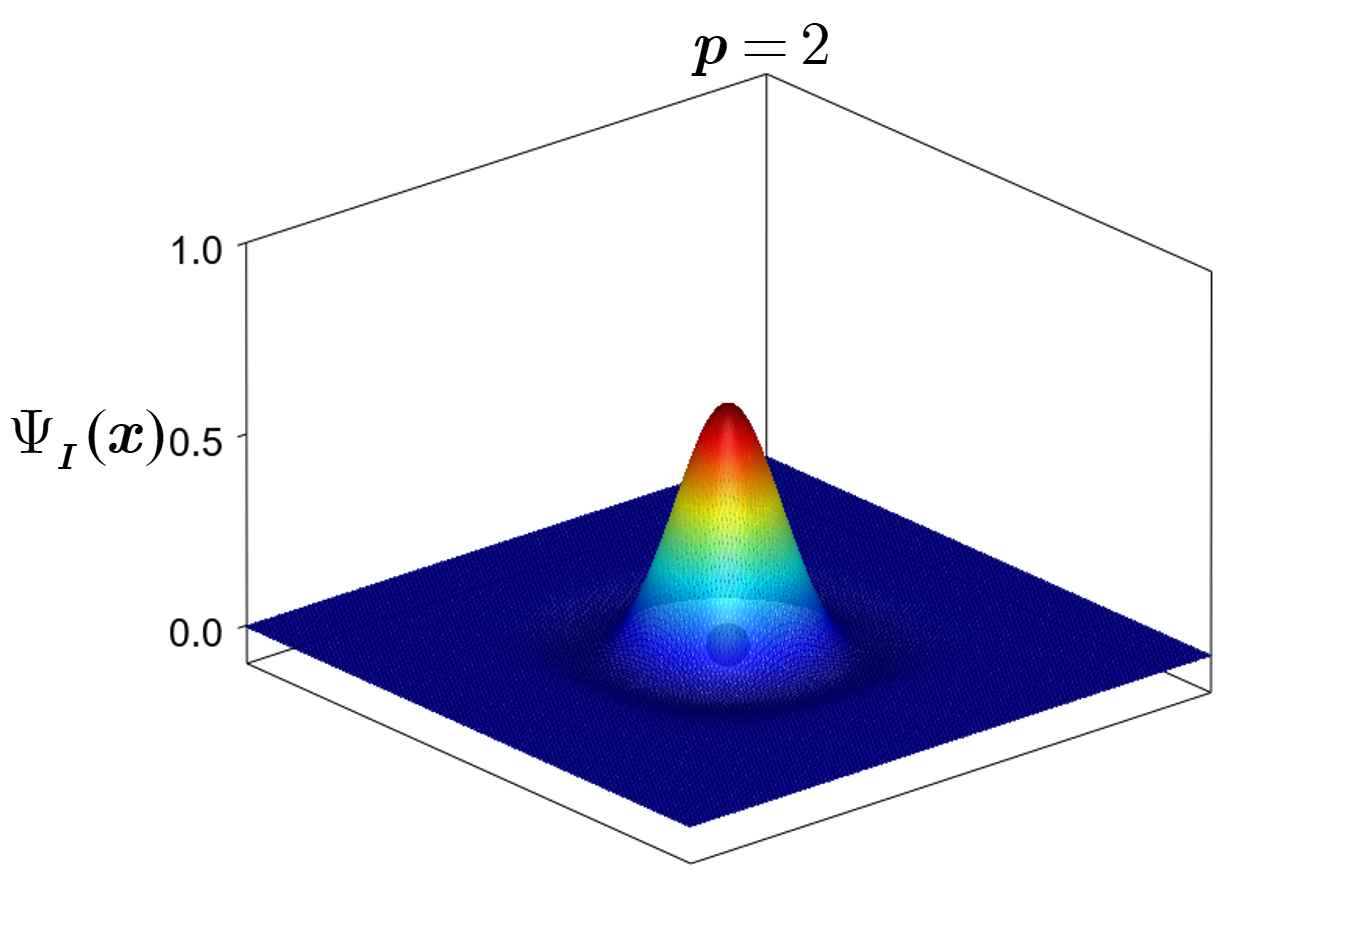
\includegraphics[width=0.3\textwidth]{figure/nomesh/QD41/1.png}
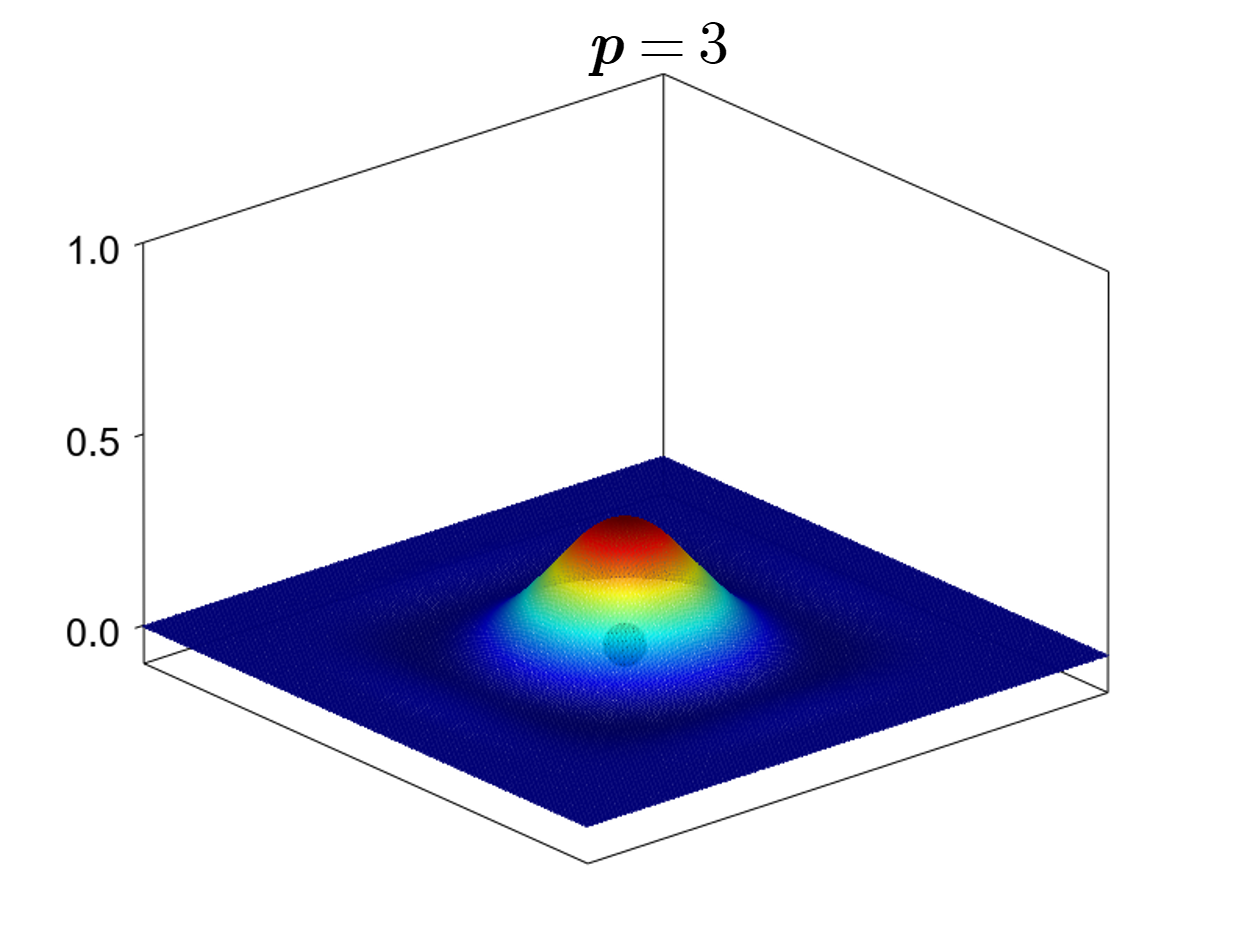
\includegraphics[width=0.3\textwidth]{figure/nomesh/C41/1.png}
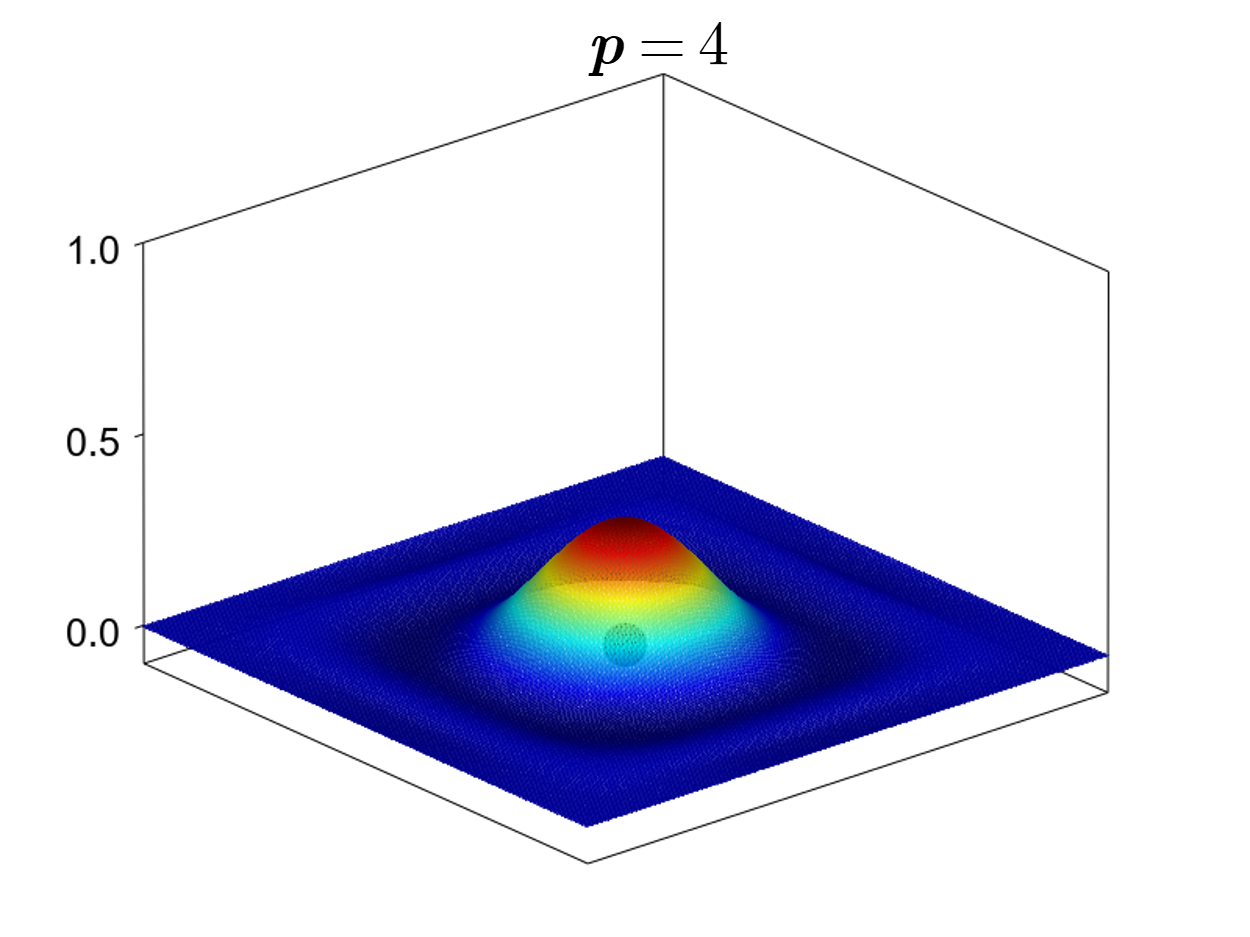
\includegraphics[width=0.3\textwidth]{figure/nomesh/QT41/1.png}
\end{subcaptiongroup}
 \begin{subcaptiongroup}
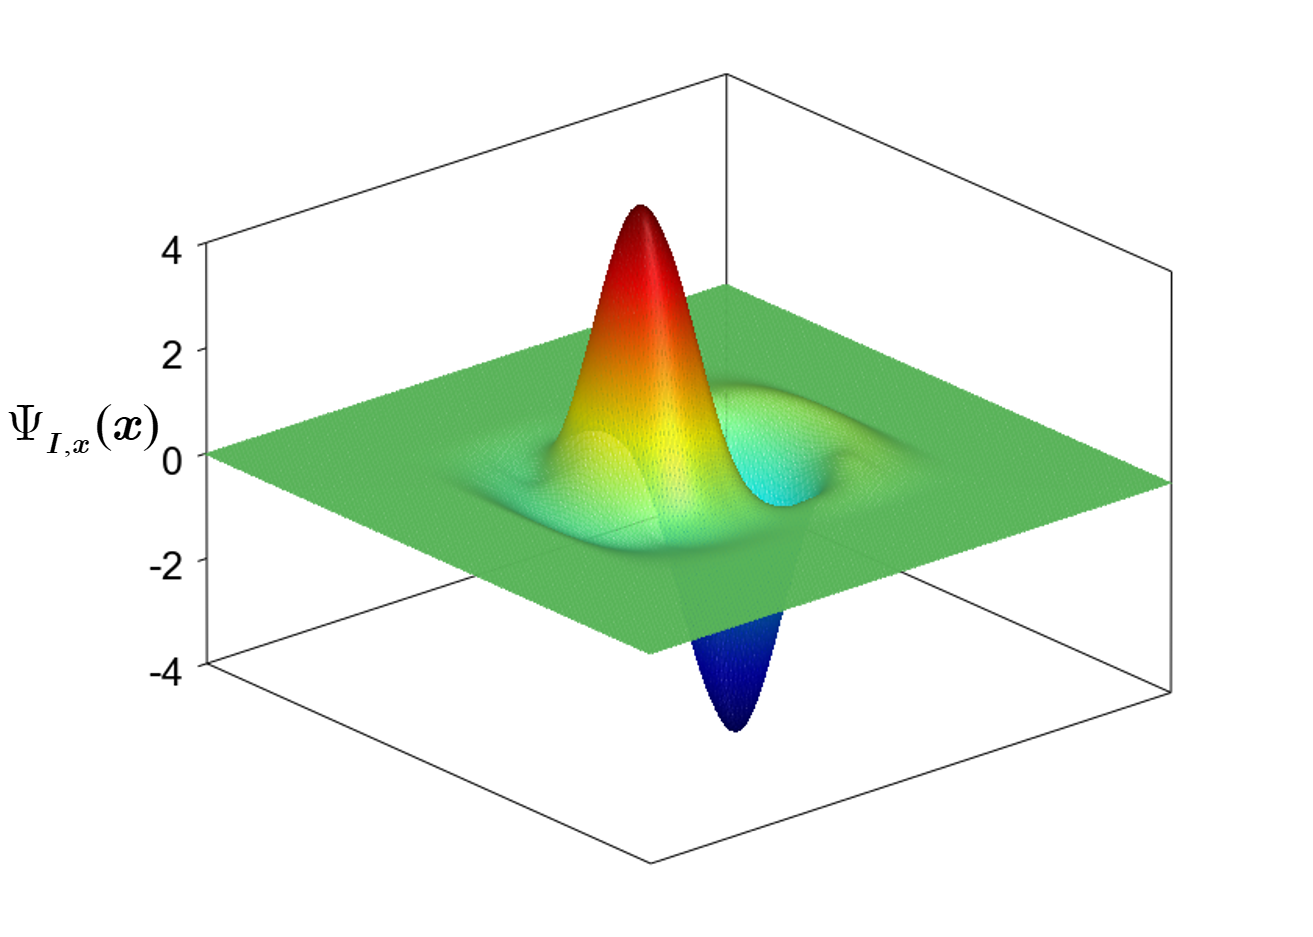
\includegraphics[width=0.3\textwidth]{figure/nomesh/QD41/2.png}
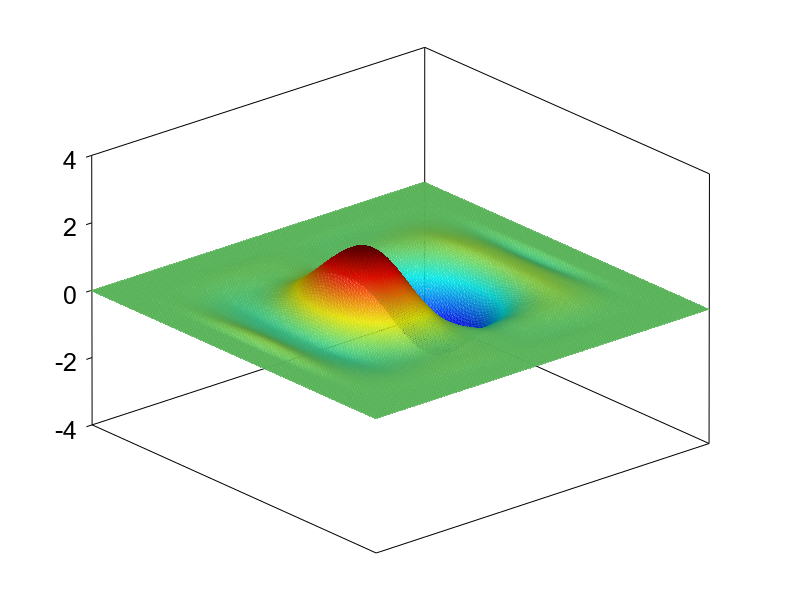
\includegraphics[width=0.3\textwidth]{figure/nomesh/C41/2.png}
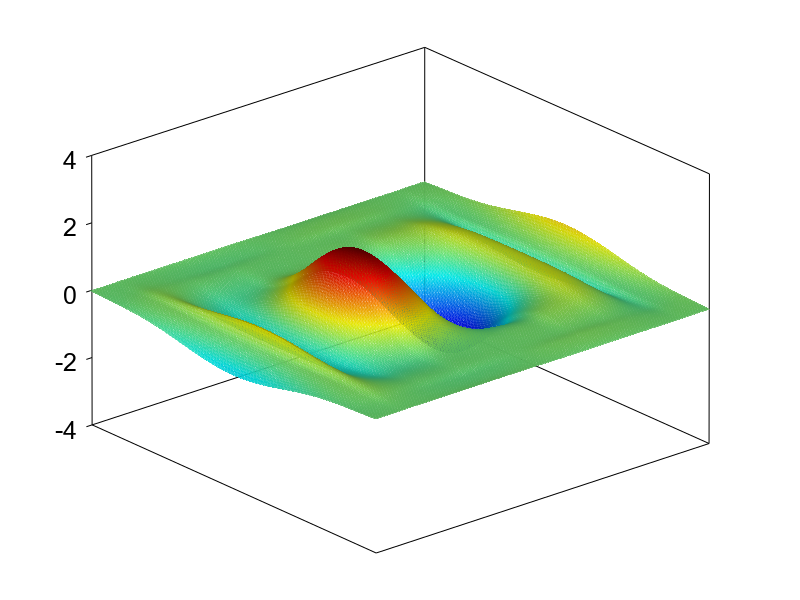
\includegraphics[width=0.3\textwidth]{figure/nomesh/QT41/2.png}
\end{subcaptiongroup}
\begin{subcaptiongroup}
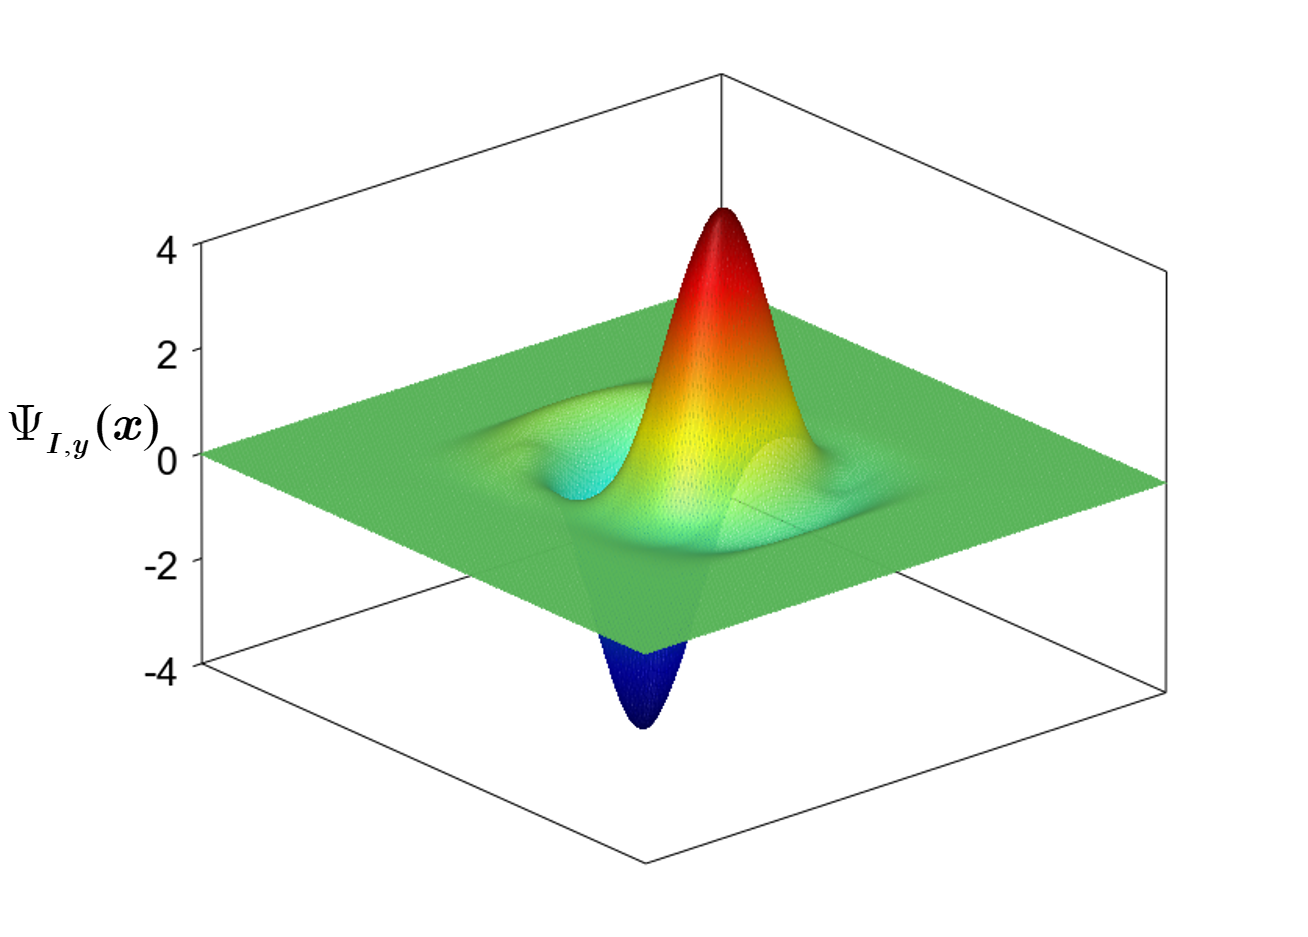
\includegraphics[width=0.3\textwidth]{figure/nomesh/QD41/3.png}
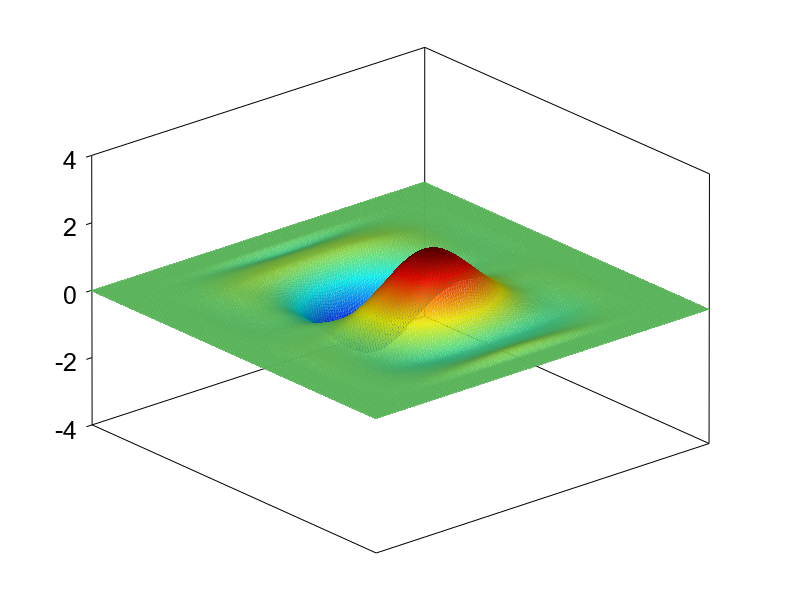
\includegraphics[width=0.3\textwidth]{figure/nomesh/C41/3.png}
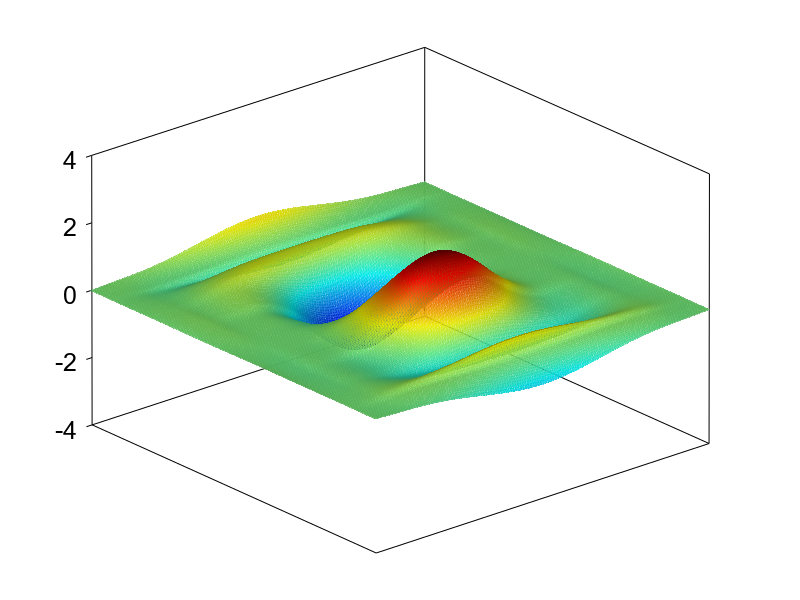
\includegraphics[width=0.3\textwidth]{figure/nomesh/QT41/3.png}
\end{subcaptiongroup}
\begin{subcaptiongroup}
    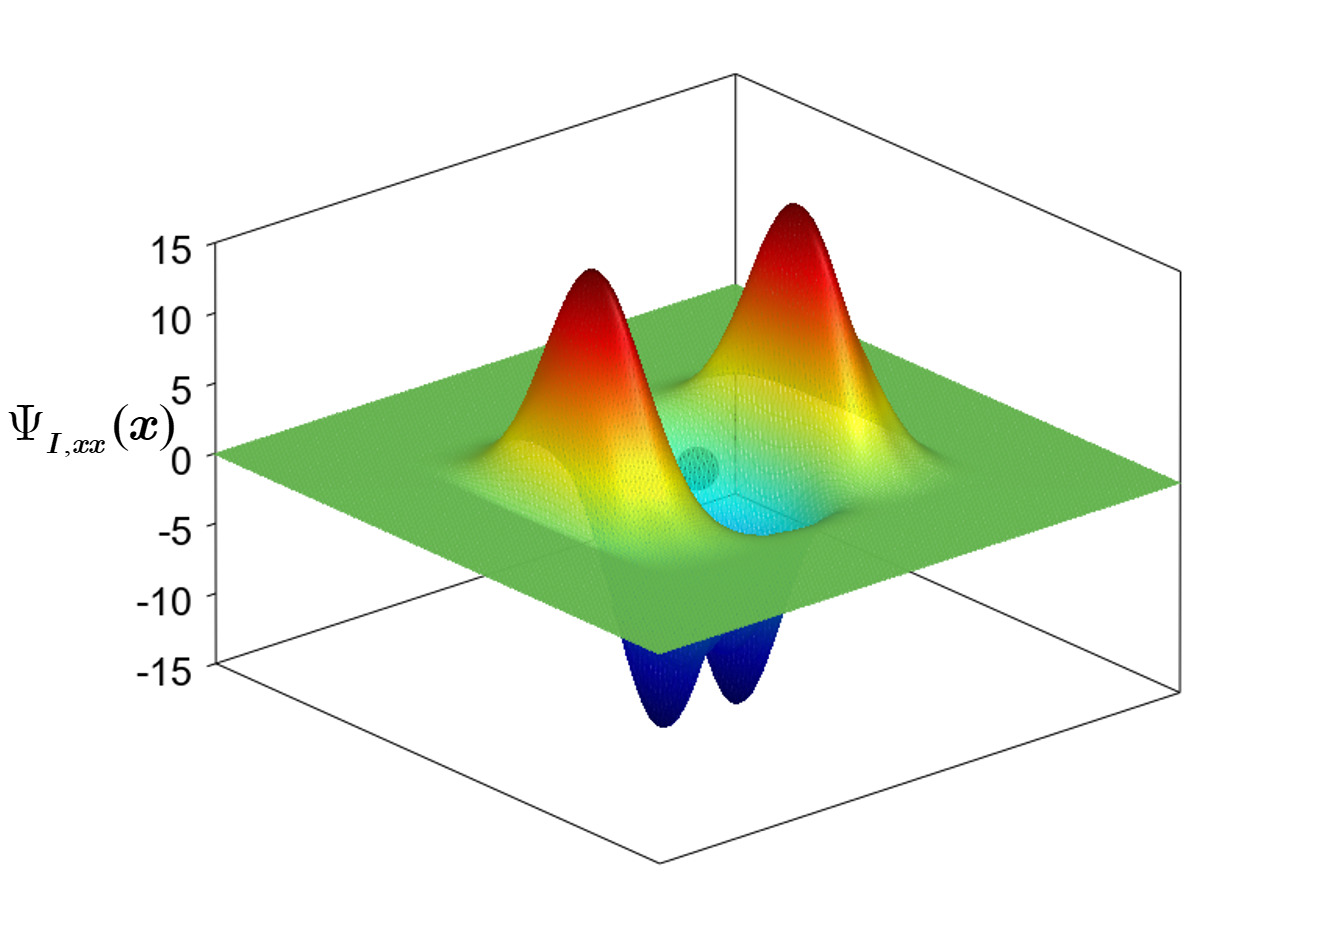
\includegraphics[width=0.3\textwidth]{figure/nomesh/QD41/4.png}
    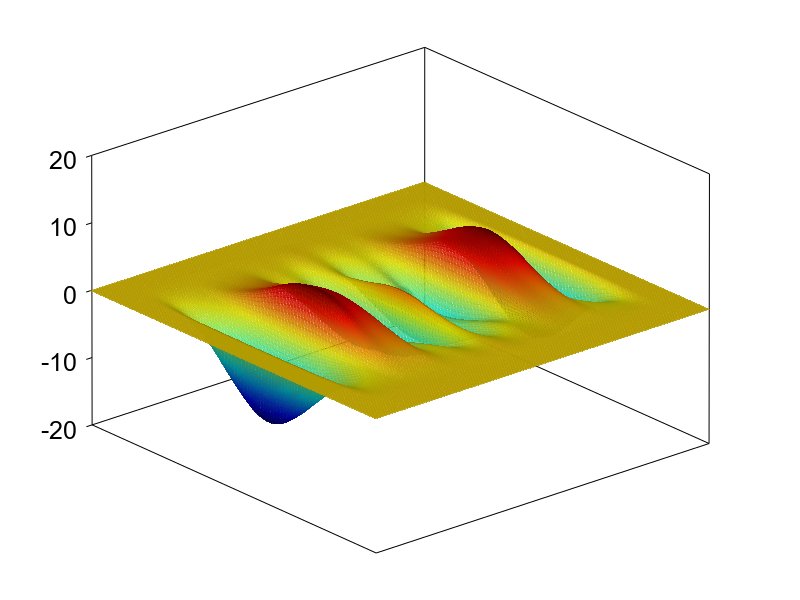
\includegraphics[width=0.3\textwidth]{figure/nomesh/C41/4.png}
    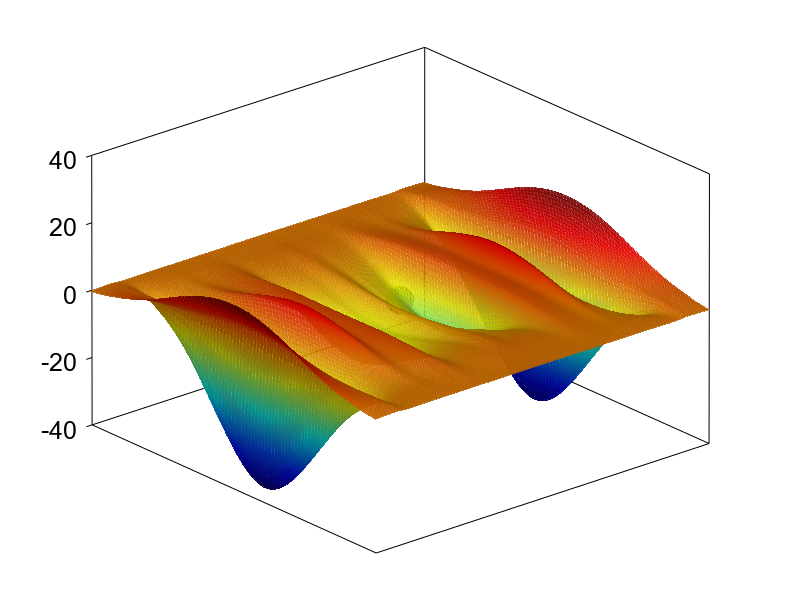
\includegraphics[width=0.3\textwidth]{figure/nomesh/QT41/4.png}
\end{subcaptiongroup}
\begin{subcaptiongroup}
    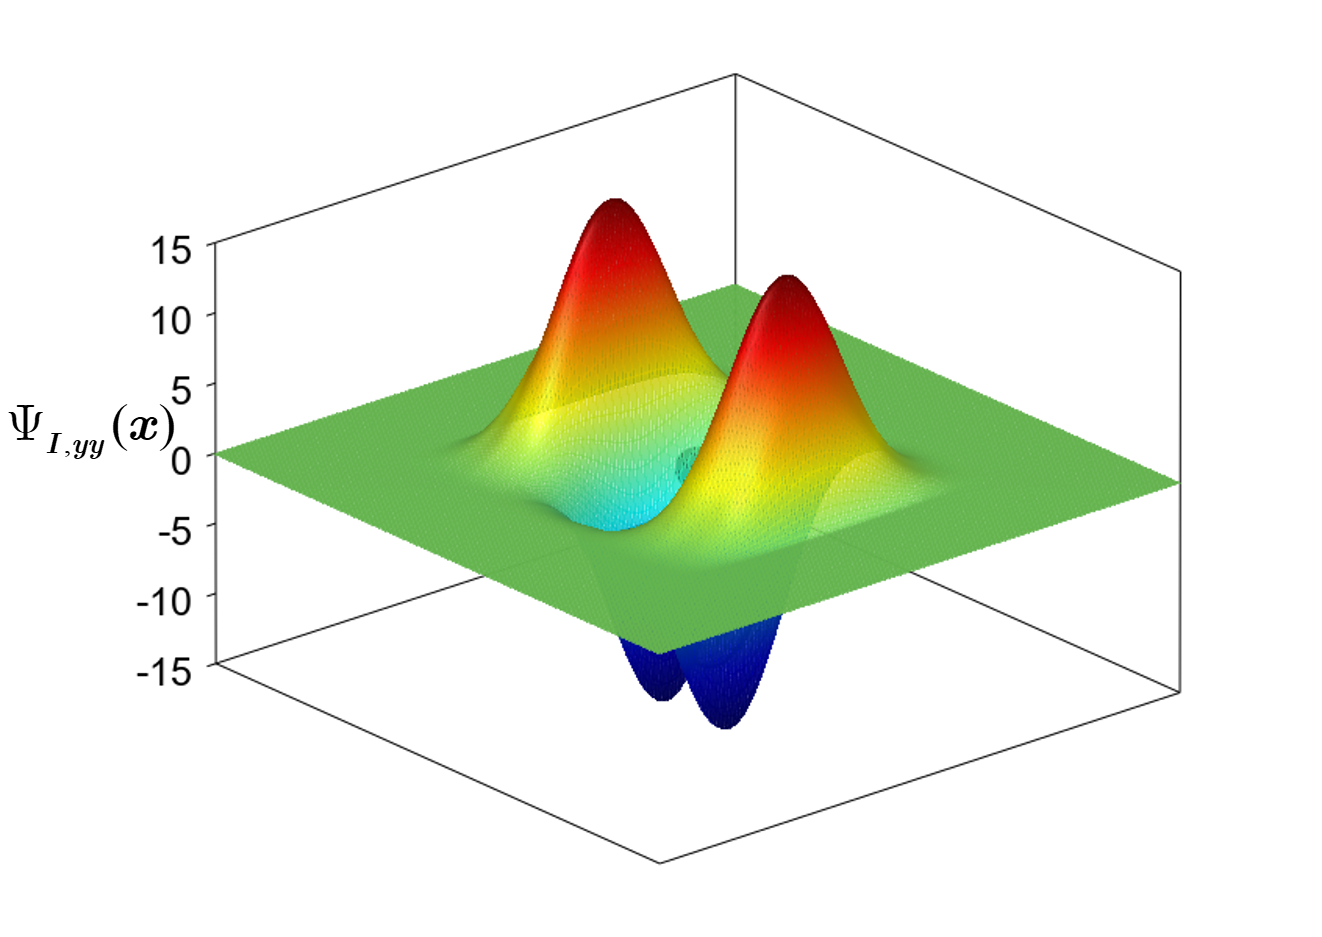
\includegraphics[width=0.3\textwidth]{figure/nomesh/QD41/5.png}
    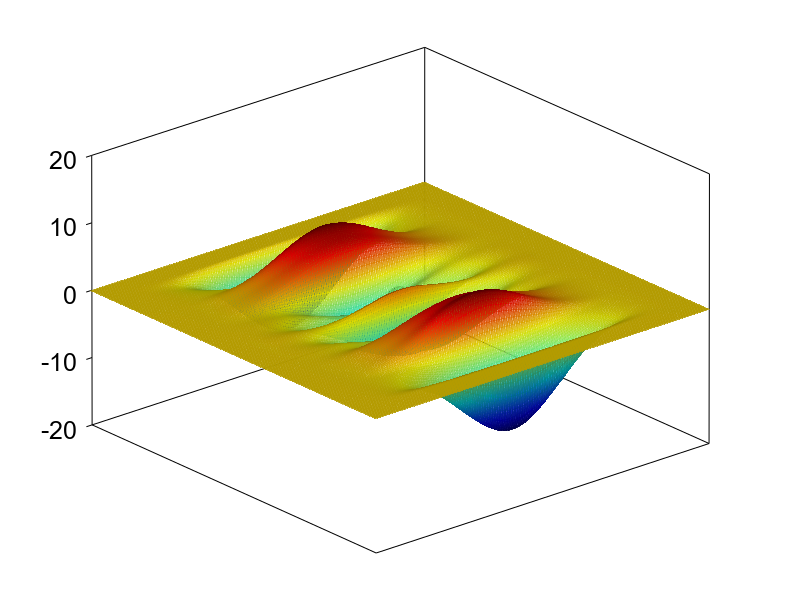
\includegraphics[width=0.3\textwidth]{figure/nomesh/C41/5.png}
    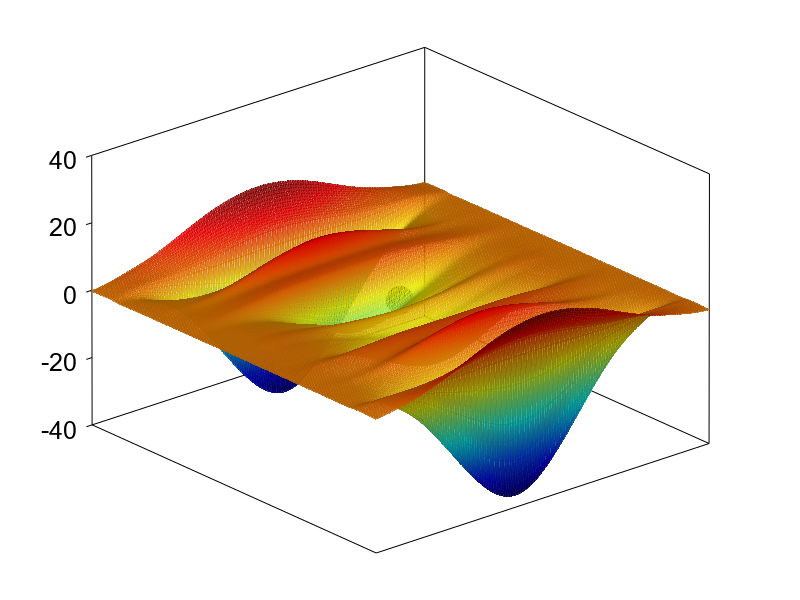
\includegraphics[width=0.3\textwidth]{figure/nomesh/QT41/5.png}
\end{subcaptiongroup}
\caption{二维内部节点无网格形函数及其一阶导数}\label{gradient1}
\end{figure}
\begin{figure}[H]
    \centering
    \begin{subcaptiongroup}
    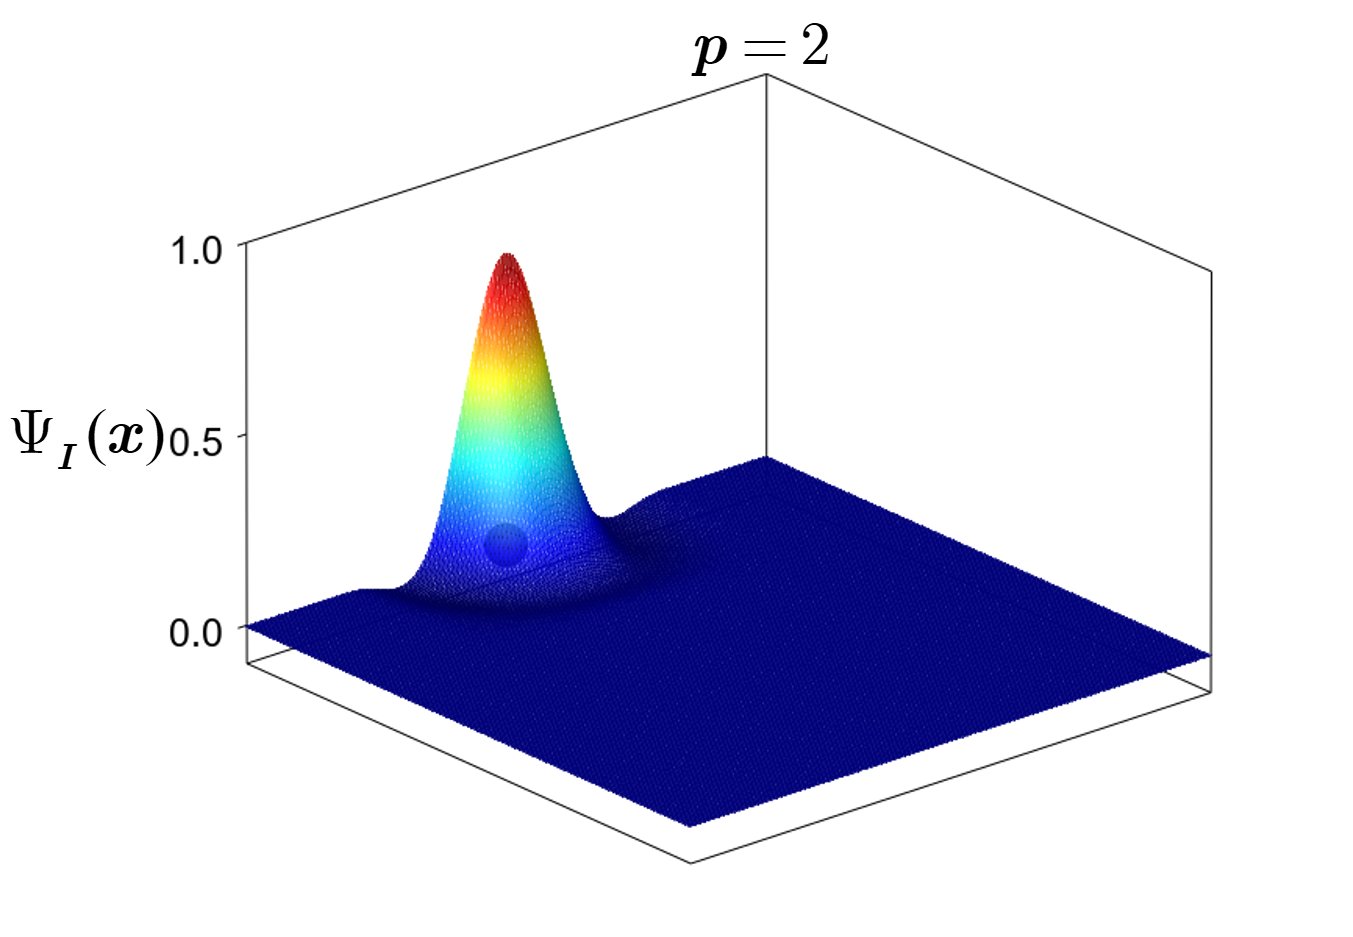
\includegraphics[width=0.3\textwidth]{figure/nomesh/QD77/1.png}
    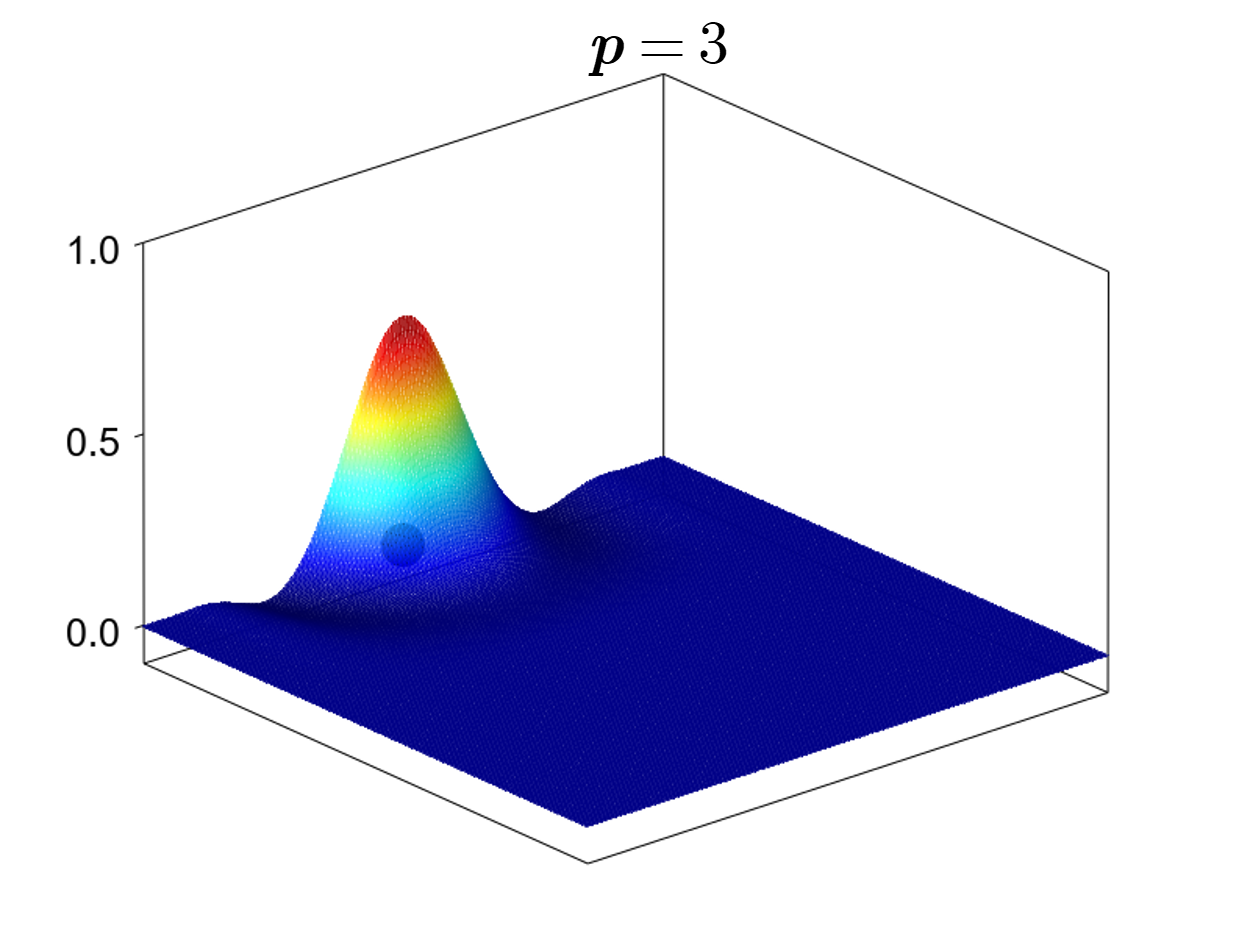
\includegraphics[width=0.3\textwidth]{figure/nomesh/C77/1.png}
    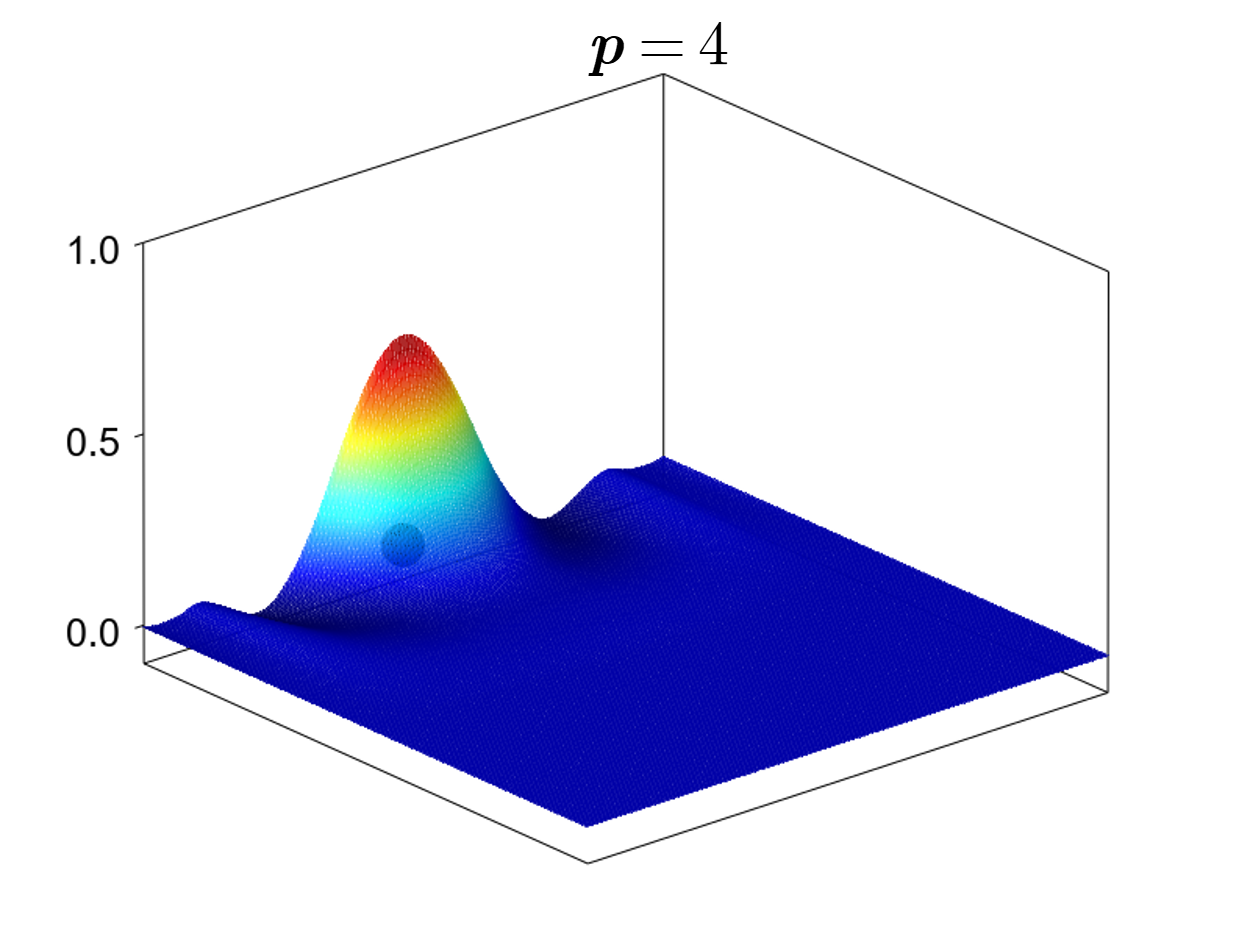
\includegraphics[width=0.3\textwidth]{figure/nomesh/QT77/1.png}
    \end{subcaptiongroup}
     \begin{subcaptiongroup}
    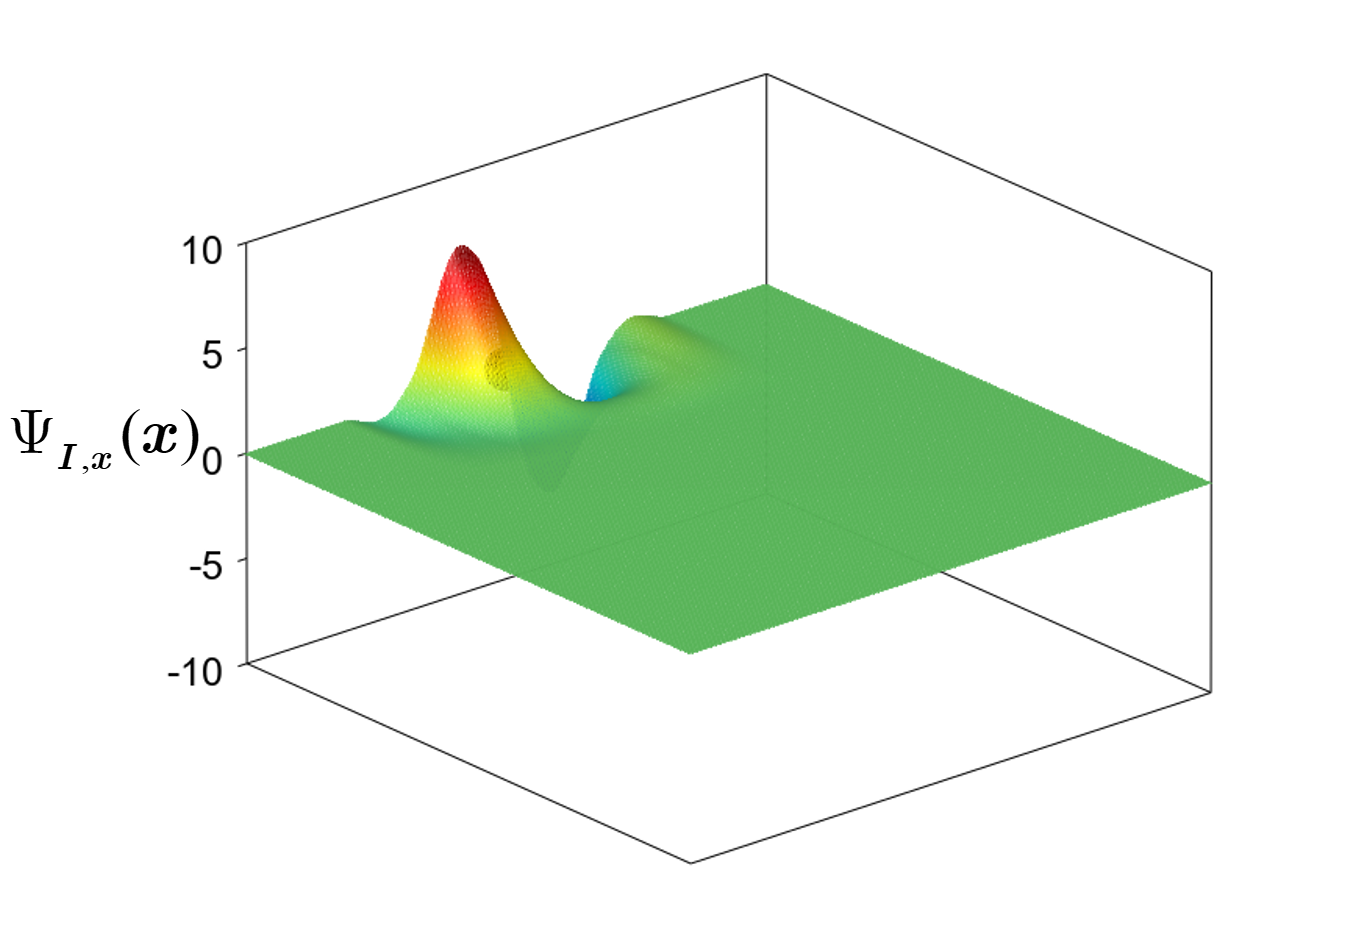
\includegraphics[width=0.3\textwidth]{figure/nomesh/QD77/2.png}
    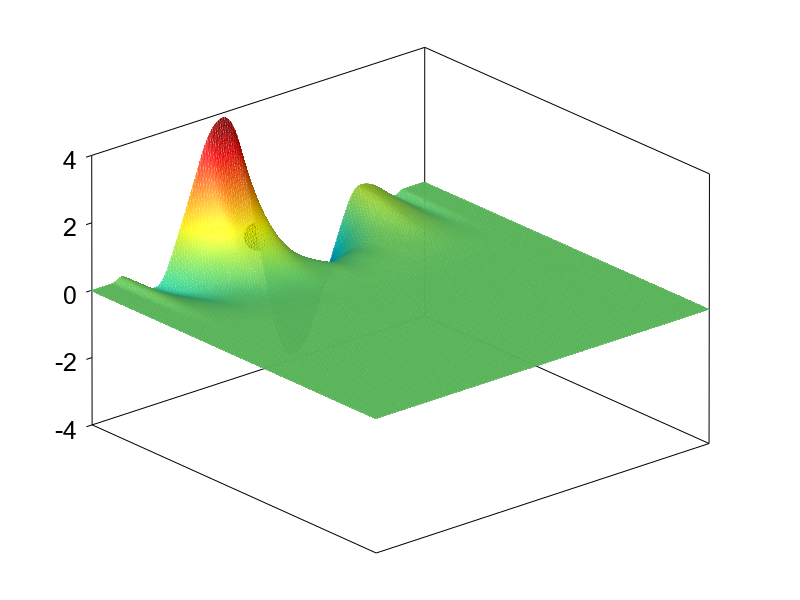
\includegraphics[width=0.3\textwidth]{figure/nomesh/C77/2.png}
    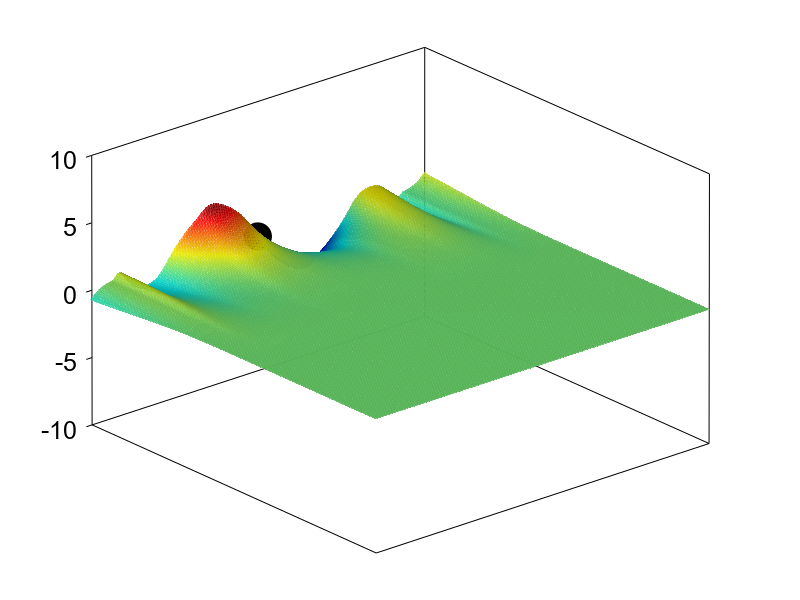
\includegraphics[width=0.3\textwidth]{figure/nomesh/QT77/2.png}
    \end{subcaptiongroup}
    \begin{subcaptiongroup}
    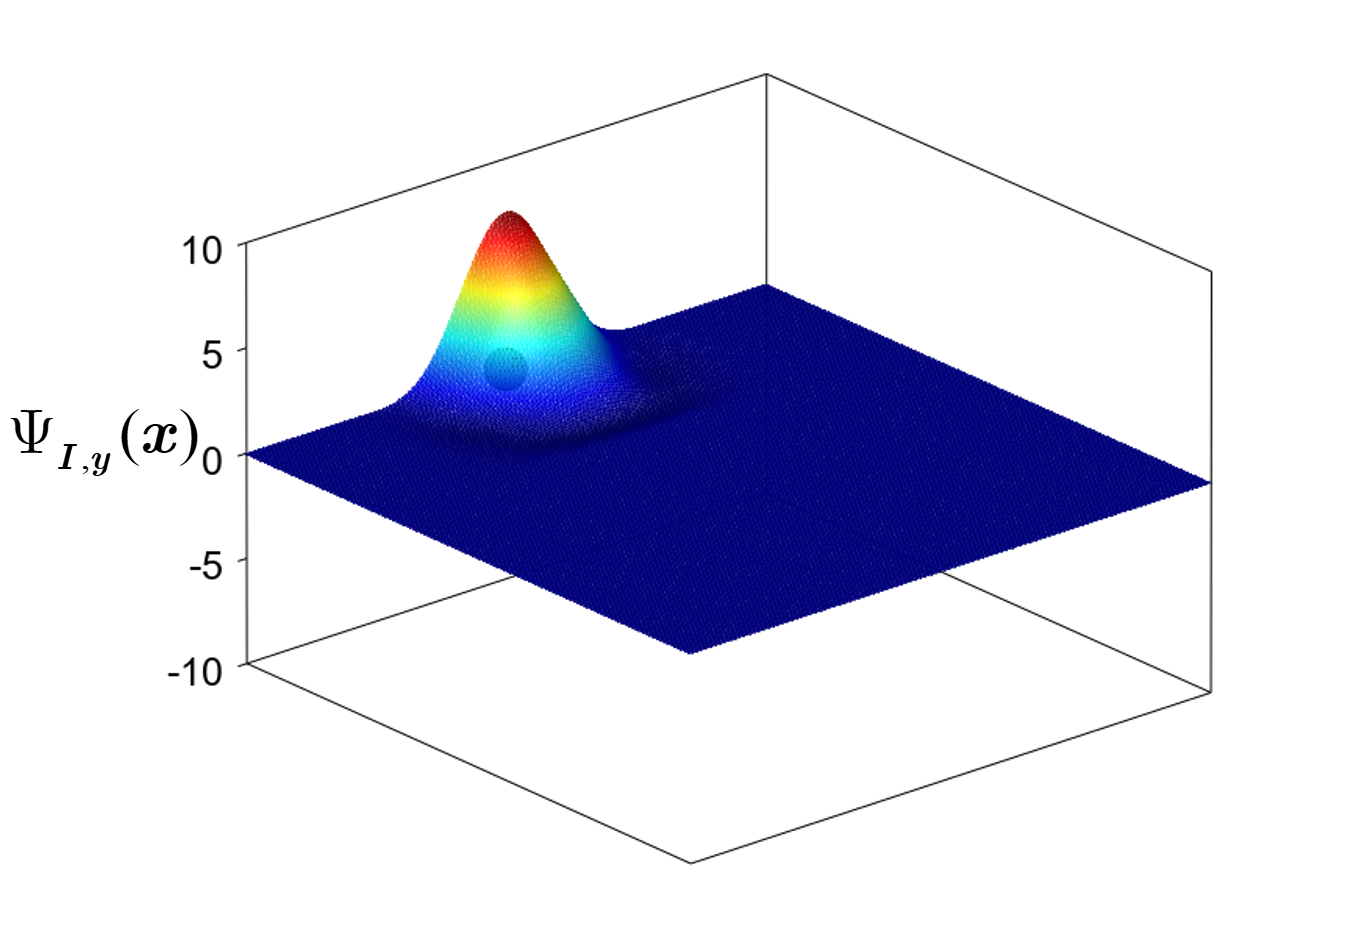
\includegraphics[width=0.3\textwidth]{figure/nomesh/QD77/3.png}
    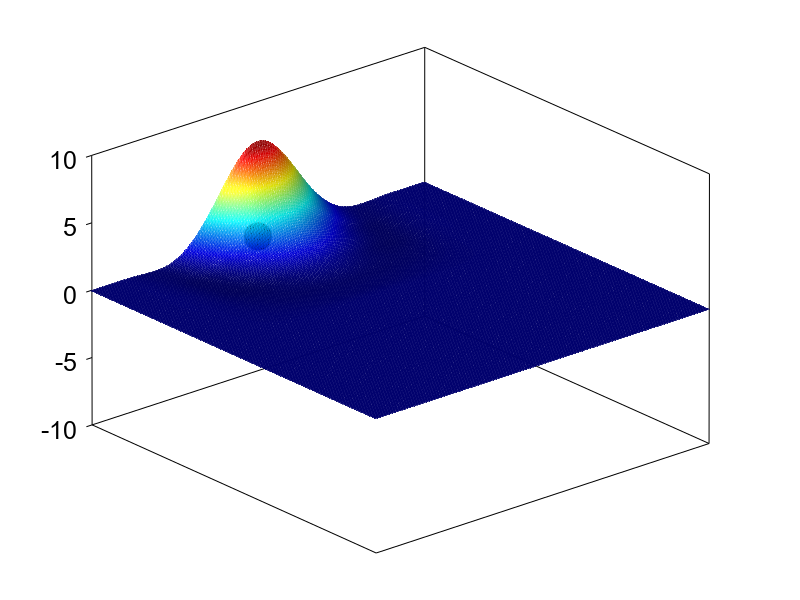
\includegraphics[width=0.3\textwidth]{figure/nomesh/C77/3.png}
    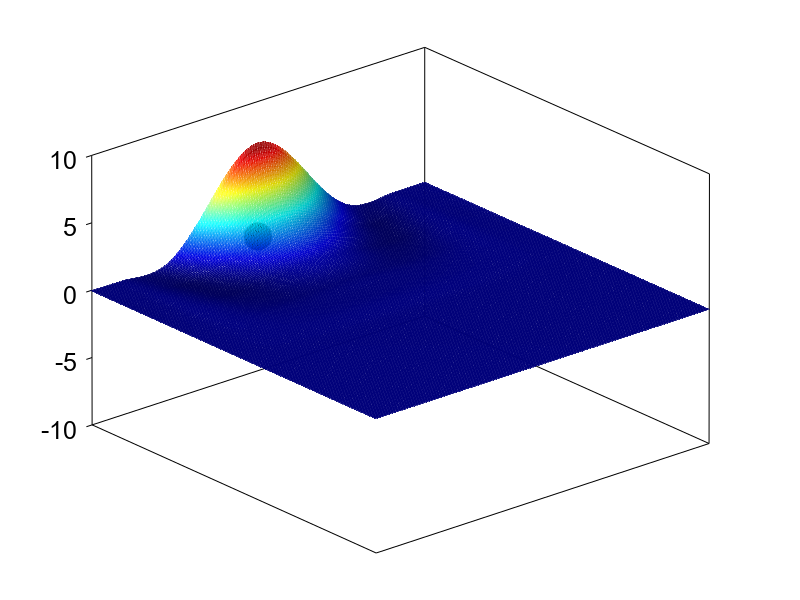
\includegraphics[width=0.3\textwidth]{figure/nomesh/QT77/3.png}
    \end{subcaptiongroup}
    \begin{subcaptiongroup}
        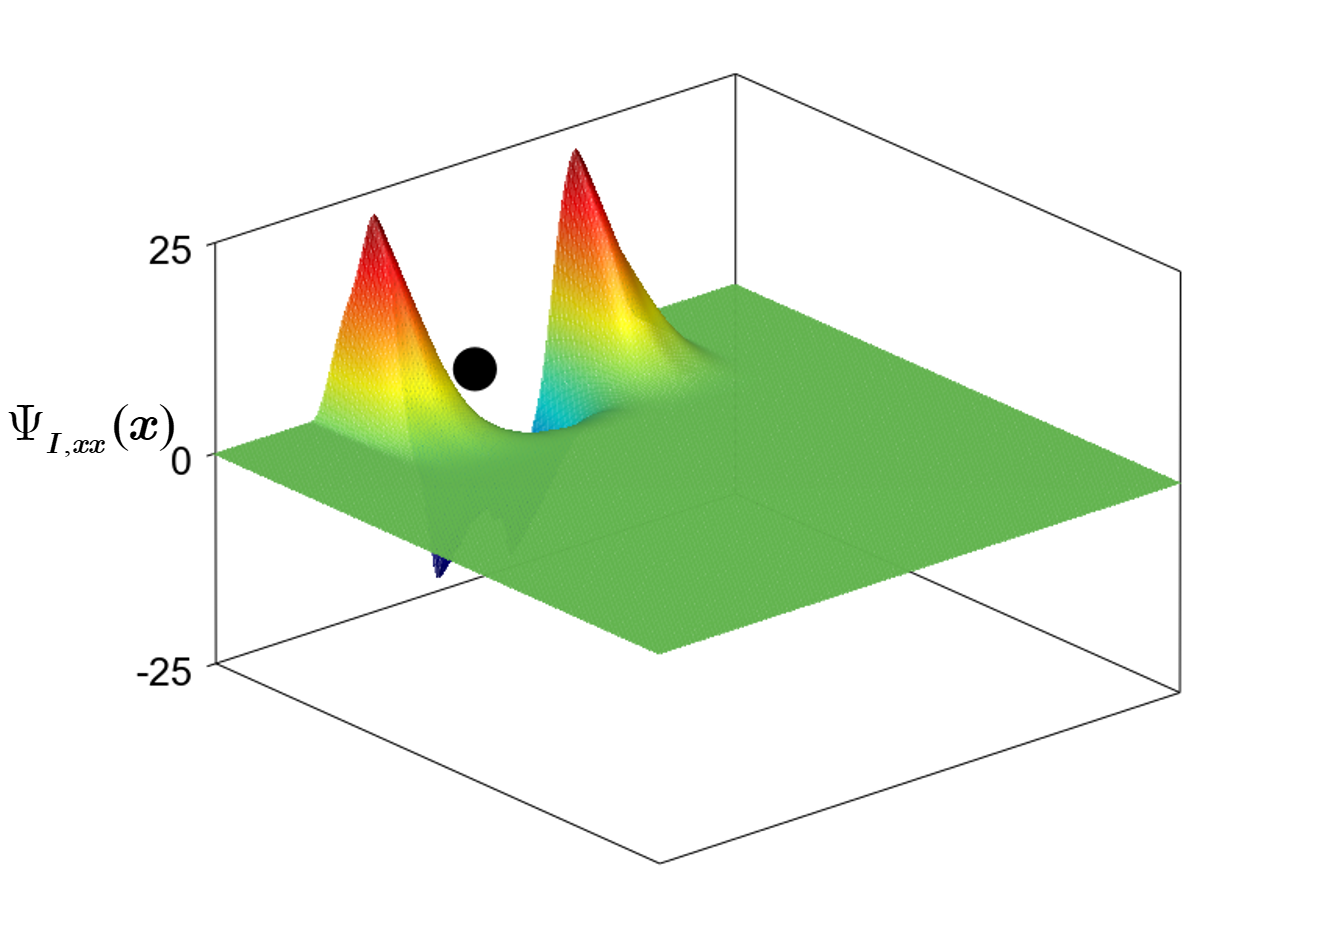
\includegraphics[width=0.3\textwidth]{figure/nomesh/QD77/4.png}
        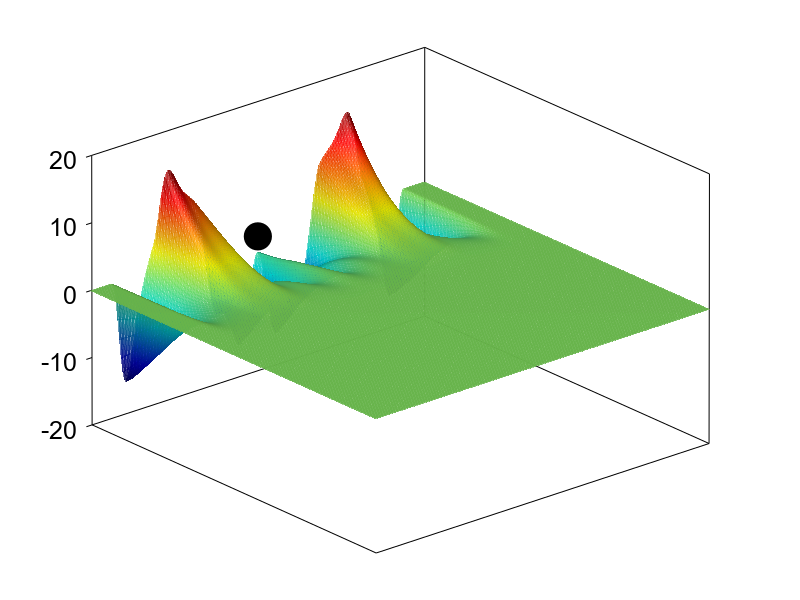
\includegraphics[width=0.3\textwidth]{figure/nomesh/C77/4.png}
        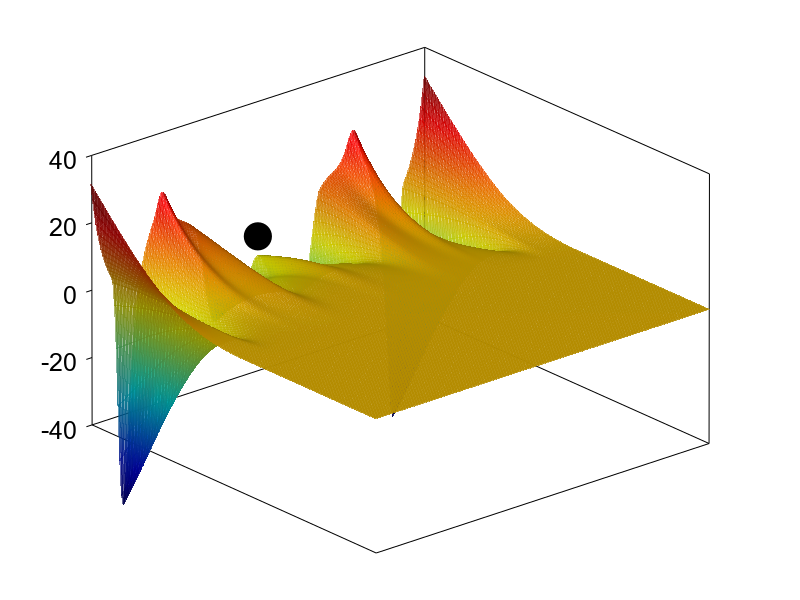
\includegraphics[width=0.3\textwidth]{figure/nomesh/QT77/4.png}
    \end{subcaptiongroup}
    \begin{subcaptiongroup}
        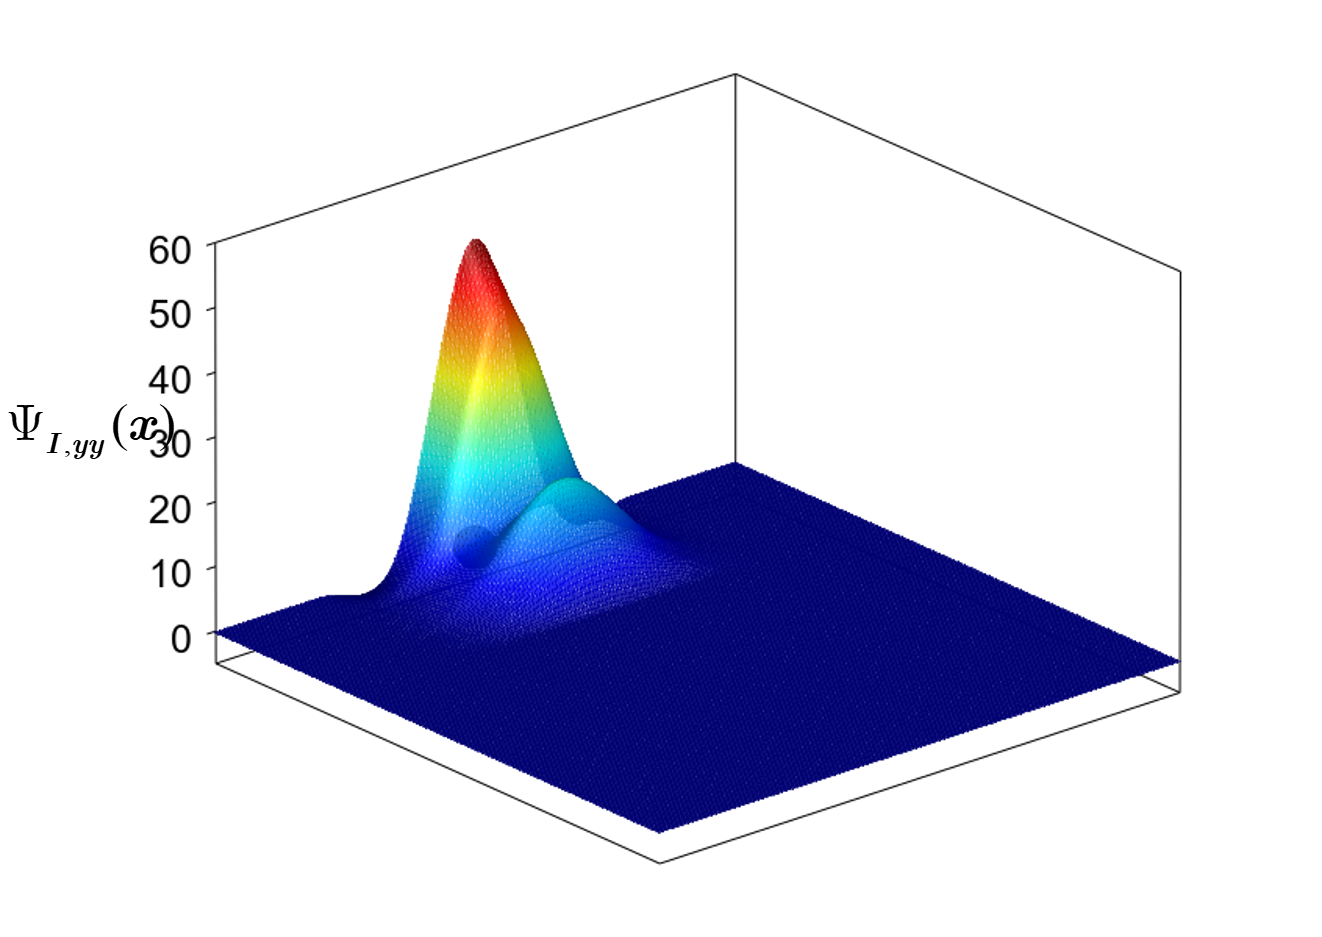
\includegraphics[width=0.3\textwidth]{figure/nomesh/QD77/5.png}
        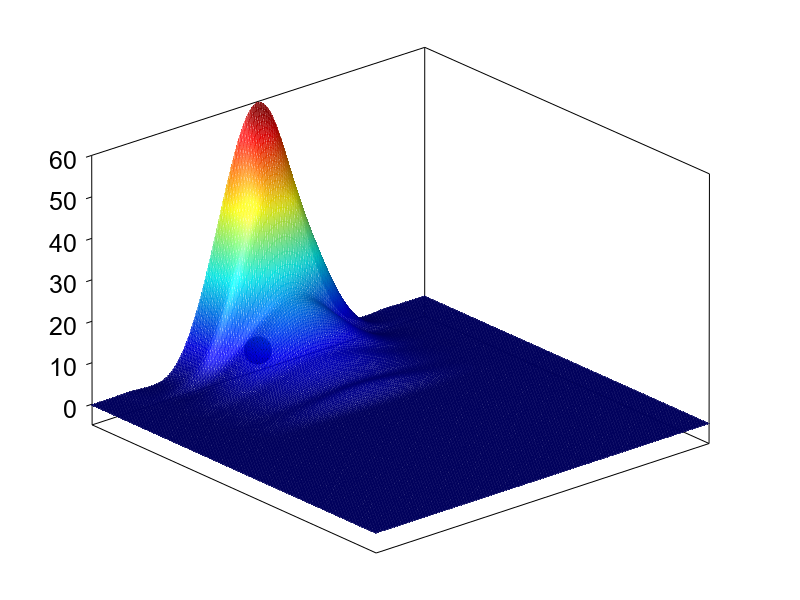
\includegraphics[width=0.3\textwidth]{figure/nomesh/C77/5.png}
        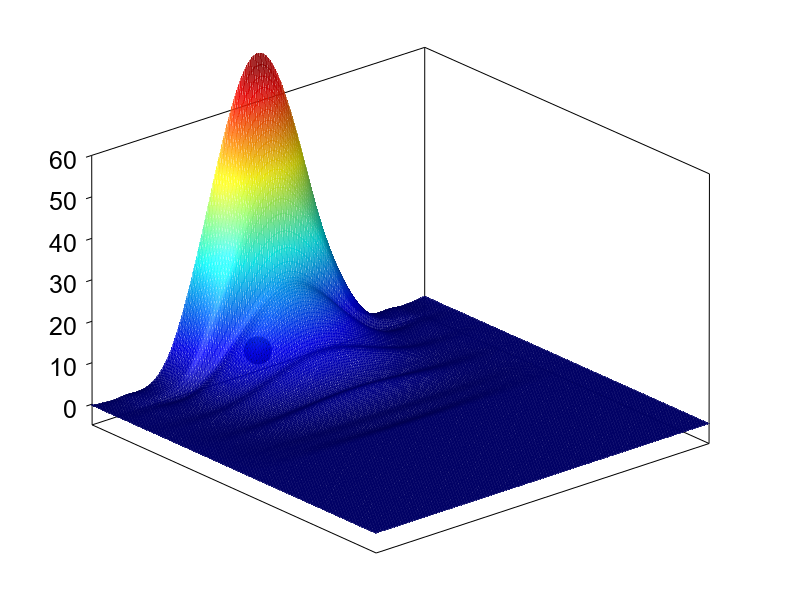
\includegraphics[width=0.3\textwidth]{figure/nomesh/QT77/5.png}
    \end{subcaptiongroup}
\caption{二维边界点处无网格形函数及其一阶导数}\label{gradient2}
\end{figure}
图(\ref{gradient1})、(\ref{gradient2})分别为内部节点和边界点处的无网格形函数及其导数图,从图中可知,无网格形函数具有全域高阶连续光滑的特点。但其无论是内部节点或边界点上的形函数在本点处均不具备插值性,即$\Psi_I(\pmb{x}_J)=\delta_{IJ}$。这将导致无网格法无法像有限元一样直接施加本质边界条件,需通过弱形式施加本质边界条件。
\newpage
\section{伽辽金无网格法}
\subsection{弹性力学问题}
不失为一般性,弹性力学问题的平衡微分方程为:
\begin{equation}\label{elasticity problems}
\begin{cases}
    \sigma_{ij,j}+b_i=0&\text{in}\;\Omega\\
    \sigma_{ij}n_j=t_i&\text{on}\;\Gamma^t\\
    u_i=g_i&\text{on}\;\Gamma^g
\end{cases}
\end{equation}
其中$\sigma_{ij}$为应力张量$\pmb \sigma$的分量,$u_i$为位移张量$\pmb{u}$的分量,$b_i$为体力张量$\pmb{b}$的分量。$\Gamma^t \text{、}\Gamma^g$分别表示自然和本质边界条件,并满足下列关系式:
\begin{equation}
\Gamma^t\cup \Gamma^g=\Gamma,\Gamma^t\cap \Gamma^g=\varnothing
\end{equation}
在自然和本质边界上具有给定的面力$\pmb{t}$和位移$\pmb{g}$,其分量分别为$t_i$和$g_i$。$n_i$为$\Gamma^{t}$上外法向量$\pmb{n}$的分量。\par
对于线弹性各向同性材料,其本构关系为:
\begin{equation}\label{constitutive relation}
    \sigma_{ij}=C_{ijkl}\varepsilon_{kl}
\end{equation}
其中$C_{ijkl}$为四阶弹性张量,$\varepsilon_{ij}$为应变张量的分量,根据小变形假设,应变$\varepsilon_{ij}$为:
\begin{equation}\label{CH2-strain}
    \varepsilon_{ij}=\frac{1}{2}(u_{i,j}+u_{j,i})
\end{equation} \par
根据最小势能原理,强形式(\ref{elasticity problems})所对应的势能泛函表达式为:
\begin{equation}\label{elasticity potential functional}
\begin{split}
    \Pi(\pmb{u})=\frac{1}{2}\int_{\Omega}\varepsilon_{ij}C_{ijkl}\varepsilon_{kl}d\Omega-\int_{\Omega}u_ib_id\Omega-\int_{\Gamma^t}u_it_id\Gamma
\end{split}
\end{equation}
对式(\ref{elasticity potential functional})进行变分可以得到式(\ref{elasticity problems})的等效积分弱形式:
\begin{equation}\label{elasticity weak form}
\begin{split}
    \delta\Pi(\pmb{u})&=\int_{\Omega}\delta\varepsilon_{ij}C_{ijkl}\varepsilon_{kl}d\Omega-\int_{\Omega}\delta u_ib_id\Omega-\int_{\Gamma^t}\delta u_it_id\Gamma=0
\end{split}
\end{equation}\par
在伽辽金无网格法中,引入无网格近似离散位移$\pmb u$及其变分$\delta \pmb u$,其近似函数$\pmb u^h$和$\delta \pmb u^h$的分量为:
\begin{equation}\label{displacement vector}
    u^h_{i}(\pmb x) = \sum_{I=1}^{N\!P}\Psi_I(\pmb x) d_{iI}, \quad \delta u^h_{i}(\pmb x) = \sum_{I=1}^{N\!P}\Psi_I(\pmb x) \delta d_{iI}
\end{equation}
式中$d_{iI}$、$\delta d_{iI}$分别为近似位移分量$u^h_i$、$\delta u^h_i$在$\pmb x_I$处的节点系数。进一步将位移表达式\ref{displacement vector}代入应变表达式\ref{CH2-strain}中可得:
\begin{equation}\label{strainh}
\varepsilon^h_{ij} = \sum_{I=1}^{N\!P} (\Psi_{I,i}d_{jI}+\Psi_{I,j}d_{iI})
\end{equation}
将式(\ref{displacement vector})、(\ref{strainh})代入到弱形式(\ref{elasticity weak form})中可以得到弹性力学问题离散控制方程式:
\begin{equation}
    \pmb{K}\pmb{d}=\pmb{f}
\end{equation}
其中$\pmb{d}=\{d_{iI}\}$表示位移节点系数向量,$\pmb{K}=\{\pmb K_{I\!J}\}$和$\pmb{f}=\{\pmb f_I\}$分别表示刚度矩阵和力向量,其分量具有表达式为:
\begin{subequations}\label{EKf}
\begin{align}
        \pmb K_{I\!J}&=\int_{\Omega}\pmb{B}_I^T\pmb{D}\pmb{B}_Jd\Omega\label{EKf1}\\
        \pmb f_I&=\int_{\Omega}\Psi_I\pmb{b}d\Omega+\int_{\Gamma^t}\Psi_I\pmb{t}d\Gamma\label{EKf2}
\end{align}
\end{subequations}
式中$\pmb B_I$为形函数梯度矩阵,$\pmb D$为材料系数矩阵。在二维平面应力和平面应变问题中,$\pmb B_I$和$\pmb D$具有如下表达式:
\begin{equation}\label{strain vector}
    \pmb{B}_I= \left[\begin{matrix}\Psi_{I,x}&0\\0&\Psi_{I,y}\\\Psi_{I,y}&\Psi_{I,x} \end{matrix}\right] 
\end{equation}
\begin{itemize}
    \item 平面应力问题
\begin{equation}\label{Dplanestress}
\pmb D = \frac{E}{1-\nu^2}\left[\begin{matrix}1&\nu&0\\\nu&1&0\\0&0&\frac{1-\nu}{2}
\end{matrix}\right] 
\end{equation}
\item 平面应变问题
\begin{equation}
\pmb D = \frac{E}{(1+\nu)(1-2\nu)}\left[\begin{matrix}1-\nu&\nu&0\\\nu&1-\nu&0\\0&0&\frac{1-2\nu}{2}
\end{matrix}\right] 
\end{equation}
\end{itemize}
\subsection{薄板问题}
考虑如图(\ref{plate})所示薄板区域$\bar \Omega$,其中板厚为$h$,$\Omega$为薄板中面。在Kirchhoff薄板假设下\cite{Liu},薄板中面的剪切变形可忽略不计,此时平衡微分方程可退化为如下形式:
\begin{equation}
    \begin{cases}\label{P control equation}
        M_{\alpha\beta,\alpha\beta}+\bar q=0&\mathrm{in} \; \Omega\\
        w=\bar w&\mathrm{on}\;\Gamma_w\\
        \theta_{\pmb n}=w_{,\pmb n}=\bar \theta_{\pmb n}&\mathrm{on}\;\Gamma_{\theta}\\
        V_{\pmb n}=Q_{\pmb n}+M_{\pmb{ns},\pmb s}=\bar V_{\pmb n}&\mathrm{on}\;\Gamma_V\\
        M_{\pmb{nn}}=\bar M_{\pmb{nn}}&\mathrm{on}\; \Gamma_M\\
        w=\bar w&\mathrm{at} \; c_w\\
        P=-\left .M_{ns} \right \vert_{c_p}=\bar P&\mathrm{at}\; c_P
    \end{cases}
\end{equation}
\begin{figure}[H]
    \centering
    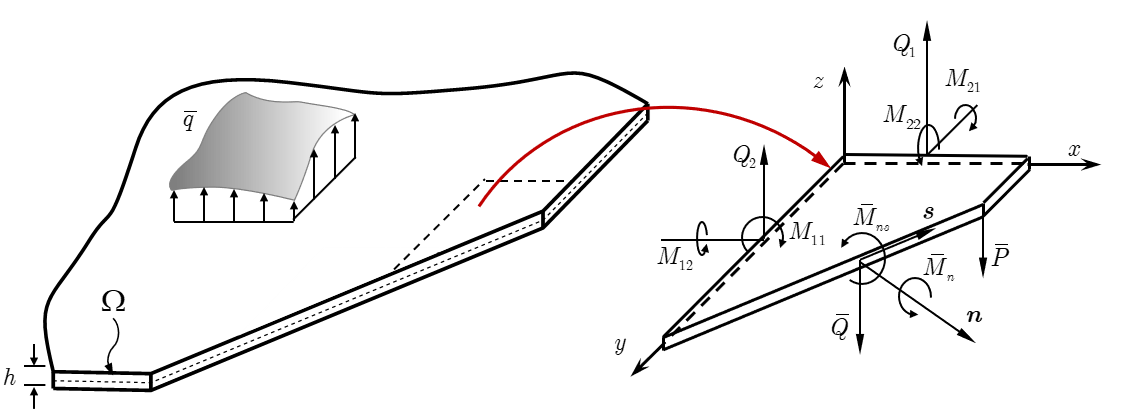
\includegraphics[scale=0.7]{figure/nomesh/plate.png}
    \caption{薄板运动学及边界条件}\label{plate}
\end{figure}
\noindent
其中
\begin{subequations}
\begin{align}
\label{wn} &w_{,\pmb n}=w_{,\alpha}n_{\alpha}\\
\label{Qn} &Q_{\pmb n}=n_{\alpha}M_{\alpha\beta,\beta}\\
\label{Mn} &M_{\pmb{nn}}=M_{\alpha\beta}n_{\alpha}n_{\beta},M_{\pmb{ns}}=M_{\alpha\beta n_{\alpha}s_{\beta}},M_{\pmb{ns,s}}=M_{\alpha\beta,\gamma}s_{\alpha}n_{\beta}s_{\gamma}
\end{align}
\end{subequations}
式中$M_{\alpha\beta}$可表示弯矩张量$\boldsymbol M$的弯曲和扭转部分的分量,$\bar q$为垂直于薄板中面的分布荷载。$\Gamma_w$、$\Gamma_{\theta}$和$c_w$为本质边界条件,$\bar w$和$\bar \theta_n$分别为本质边界条件上给定的挠度和转角。
$\Gamma_V$、$\Gamma_M$和$c_P$为自然边界条件,$V_{\boldsymbol n}$、$M_{\boldsymbol{nn}}$和$P$为自然边界上的等效剪力、法向弯矩和薄板角上的集中荷载。$n_\alpha$和$s_\alpha$分别为边界上外法线方向$\pmb{n}$和切方向$\pmb{s}$的分量。
所有的边界条件都满足如下关系式:
\begin{equation}\label{PGeometric relationships}
    \begin{split}
        \Gamma=\Gamma_w\cup\Gamma_V\cup\Gamma_{\theta}\cup\Gamma_M,c=c_w\cup c_P\\
        \Gamma_w\cap\Gamma_V=\Gamma_{\theta}\cap\Gamma_M=c_w\cap c_P=\varnothing
    \end{split}
\end{equation}\par
当薄板为线弹性各同向性材料时,其本构关系为:
\begin{equation}
    \begin{split}\label{Malphabeta}
        M_{\alpha\beta}=D_{\alpha\beta\gamma\eta}\kappa_{\gamma\eta}=-D_{\alpha\beta\gamma\eta}w_{,\gamma\eta}
    \end{split}
\end{equation}
其中$\kappa_{\alpha\beta}$为曲率张量$\pmb{\kappa}$的分量,表达式如下:
\begin{equation}\label{kappa}
    \kappa_{\alpha\beta}=-w_{,\alpha\beta}
\end{equation}
式中$D_{\alpha \beta \gamma \eta}$为薄板问题四阶弹性张量的分量,表达式如下:
\begin{equation}
    \begin{split}\label{Dalphabeta}
        D_{\alpha\beta\gamma\eta}=\bar D(\nu\delta_{\alpha\beta}\delta_{\gamma\eta}+\frac{1}{2}(1-\nu)(\delta_{\alpha\gamma}\delta_{\beta\eta}+\delta_{\alpha\gamma}\delta_{\beta\gamma}))
    \end{split}
\end{equation}
其中$\bar{D}$为抗弯刚度,抗弯刚度可由杨氏模量$E$、泊松比$\nu$和板厚$h$计算得到:
\begin{equation}\label{kangwangangdu}
    \begin{split}
    \bar D=\frac{Eh^3}{12(1-\nu^2)}
\end{split}
\end{equation}
\par
% 根据尺寸相关弹性\cite{Liu},将式(\ref{Qn})、(\ref{Mn})、(\ref{Malphabeta})、(\ref{Dalphabeta})代入式(\ref{P control equation})中可以得到自然边界上的法向弯矩$M_{\pmb{nn}}$、等效剪力$V_{\pmb{n}}$和薄板角上的集中荷载$P$的具体表达式:
% \begin{equation}
% \begin{split}\label{MVP}
%     \begin{cases}
%         M_{\pmb{nn}}=\mathcal{M}_{\alpha\beta}w_{,\alpha\beta}=-\bar{D}(\nu\delta_{\alpha\beta}+(1-\nu)n_{\alpha}n_{\beta})w_{,\alpha\beta}\\
%         V_{\pmb{n}}=\mathcal{V}_{\alpha\beta}w_{,\alpha\beta}=-\bar{D}(\frac{\partial}{\partial x_{\alpha}}n_{\beta}+(1-\nu)n_{\alpha}\frac{\partial}{\partial y_{\gamma}}s_{\alpha}n_{\beta}s_{\gamma})w_{,\alpha\beta}\\
%         P=\mathcal{P}_{\alpha\beta}w_{,\alpha\beta}=-[[(\bar{D}(1-\nu)n_{\alpha}s_{\beta})w_{,\alpha\beta}]]
%     \end{cases}
% \end{split}
% \end{equation}
% 其中:
% \begin{equation}
% \begin{split}\label{MVP1}
%     \begin{cases}
%  \mathcal{M}_{\alpha\beta}w_{,\alpha\beta}=-D_{\alpha\beta\gamma\eta}n_{\gamma}n_{\eta}=-\bar{D}(\nu\delta_{\alpha\beta}+(1-\nu)n_{\alpha}n_{\beta})\\
%   \mathcal{V}_{\alpha\beta}w_{,\alpha\beta}=-D_{\alpha\beta\gamma\eta}(n_{\gamma}\frac{\partial}{\partial x_{\eta}}+s_{\gamma}n_{\eta}s_{\xi}\frac{\partial}{\partial x_{\xi}})=-\bar{D}(\frac{\partial}{\partial x_{\alpha}}n_{\beta}+(1-\nu)n_{\alpha}\frac{\partial}{\partial y_{\gamma}}s_{\alpha}n_{\beta}s_{\gamma})\\
%  \mathcal{P}_{\alpha\beta}w_{,\alpha\beta}=-[[D_{\alpha\beta}n_{\gamma}s_{\eta}]]=-[[\bar{D}(1-\nu)n_{\alpha}s_{\beta}]]
%     \end{cases}
% \end{split}
% \end{equation}\par
根据最小势能原理,强形式(\ref{P control equation})所对应的的势能泛函表达式为:
\begin{equation}\label{Pshineng}
    \Pi(w)=\int_{\Omega}\frac{1}{2}\kappa_{,\alpha\beta}M_{\alpha\beta}d\Omega+\int_{\Gamma_M}\theta_{\pmb{n}}\bar{M}_{\pmb{nn}}d\Gamma
    -\int_{\Gamma_V}w\bar{V}_{\pmb{n}}d\Gamma-w\bar{P}\vert_{x\in c_P}+\int_{\Omega}w\bar{q}d\Omega
\end{equation}
对式(\ref{Pshineng})进行变分可以得到式(\ref{P control equation})的等效积分弱形式:
\begin{equation}\label{Pweakform}
\begin{split}
        \delta\Pi(w)&=\int_{\Omega}\delta\kappa_{,\alpha\beta}M_{\alpha\beta}d\Omega+\int_{\Gamma_M}\delta\theta_{\pmb{n}}\bar{M}_{\pmb{nn}}d\Gamma\\
        &-\int_{\Gamma_V}\delta w\bar{V}_{\pmb{n}}d\Gamma-\delta w\bar{P}\vert_{x\in c_P}+\int_{\Omega}\delta w\bar{q}d\Omega=0
\end{split}
\end{equation}\par
在伽辽金无网格法中,引入无网格近似离散挠度$w$及其变分$\delta w$,其近似函数$w^h$和$\delta w^h$的分量为:
\begin{equation}
\label{Pwuwangelisan}
    w_{\alpha\beta}^h(\pmb{x})=\sum_{I=1}^{N\!P}\Psi_I(\pmb{x})d_I,\quad \delta w_{\alpha\beta}^h(\pmb{x})=\sum_{I=1}^{N\!P}\Psi_I(\pmb{x})\delta d_I
\end{equation}
式中$d_I$、$\delta d_I$分别为近似挠度分量$w_{\alpha\beta}^h$、$\delta w_{\alpha\beta}^h$在$w$处的节点系数。进一步将挠度表达式(\ref{Pwuwangelisan})代入曲率张量表达式(\ref{kappa})中可得:
\begin{equation}
\kappa_{\alpha\beta}=-\sum_{I=1}^{N\!P}\Psi_{I,\alpha\beta}d_I
% \pmb{B}_I(\pmb{x})= \left[\begin{matrix}\Psi_{I,xx}\\\Psi_{I,yy}\\2\Psi_{I,xy}\end{matrix}\right] 
\end{equation}\par
将式(\ref{wn})、(\ref{Malphabeta})和(\ref{Pwuwangelisan})代入到伽辽金弱形式(\ref{Pweakform})中得到薄板问题离散平衡控制方程:
\begin{equation}
     \pmb{K}\pmb{d}=\pmb{f}
\end{equation}
其中刚度矩阵$\boldsymbol K$和力向量$\pmb f$的分量$K_{IJ}$、$f_I$分别为:
\begin{subequations}\label{PKf}
\begin{align}
    \label{PKf1}K_{I\!J}&=\frac{h^3}{12}\int_{\Omega}\pmb{B}^T_I\pmb{D}\pmb{B}_Jd\Omega\\
    \label{PKf2}f_I&=\int_{\Gamma_V}\Psi_I\bar{V}_{\pmb{n}}d\Gamma-\int_{\Gamma_M}\Psi_{I,\pmb{n}}\bar{M}_{\pmb{nn}}d\Gamma+\Psi_I\bar{P}\vert_{x\in c_P}+\int_{\Omega}\Psi_I\bar{q}d\Omega
\end{align}
\end{subequations}
式中$\pmb{D}$为式\ref{Dplanestress}中的材料系数矩阵,$\pmb{B}_I$为形函数梯度向量,其形函数梯度矩阵具有如下表达式:
\begin{equation}
\pmb{B}_I(\pmb{x})= \begin{Bmatrix}\Psi_{I,xx}\\\Psi_{I,yy}\\2\Psi_{I,xy}\end{Bmatrix} 
\end{equation}
\section{小结}
本章首先对再生核无网格近似理论进行了系统讨论,详细说明了无网格形函数及其梯度的构造过程,验证了再生核近似形函数的一致性条件。
与传统有限元形函数不同,无论是内部节点还是边界节点,再生核无网格形函数通常不具备插值性。在伽辽金法的求解过程中,无法直接施加本质边界条件,需采用弱形式的途径进行施加。
最后,以弹性力学问题和薄板问题为例,详细介绍了伽辽金无网格法在这两类问题上的离散控制方程。下一章节将以这两类问题为例,介绍主要的无网格本质边界施加方案。

\chapter{强制边界条件施加方法}
由于无网格形函数通常不具备插值特性,因此在使用无网格方法进行离散化时,需要采用适当的方法来施加强制边界条件。
在本章中,将以弹性力学问题和薄板问题为例,对常见的边界条件施加方法进行详细讨论,了解在无网格方法中如何适应边界条件的施加。

\section{拉格朗日乘子法}
Belytschko等人\cite{}提出采用拉格朗日乘子法施加本质边界条件,拉格朗日乘子法是一种常用的强制边界条件施加方法,用于在数值计算中处理约束条件。
该方法的基本思想是通过引入拉格朗日乘子,将边界条件转化为约束条件,并将其纳入数值问题的势能泛函中,通过对增广拉格朗日函数进行求解,可以同时求解原始问题和约束条件,从而获得满足边界条件的数值解。\par
弹性力学问题中拉格朗日乘子法的势能泛函表达式为:
\begin{equation}\label{Elambda}
\begin{split}
    \bar{\Pi}(\pmb{u},\pmb{\lambda})=\Pi(\pmb{u})-\int_{\Gamma^g}\pmb{\lambda}(u_i-g_i)d\Gamma
\end{split}
\end{equation}   
其中$\pmb{\lambda}=\{\lambda_1,\dotsb,\lambda_{n_{sd}}\}^T$为拉格朗日乘子,对式(\ref{Elambda})进行变分得到伽辽金弱形式:
\begin{equation}\label{Elambda weakform}
\begin{split}
        \delta\bar{\Pi}(\pmb{u},\pmb{\lambda})&=\Pi(\pmb{u})-\int_{\Gamma^g}\delta u_i\pmb{\lambda}d\Gamma-\int_{\Gamma^g}\delta\pmb{\lambda}(u_i-g_i)d\Gamma\\
       &=\int_{\Omega}\delta\varepsilon_{ij}C_{ijkl}\varepsilon_{kl}-\int_{\Omega}\delta u_ib_id\Omega-\int_{\Gamma^t}\delta u_it_id\Gamma\\
       &-\int_{\Gamma^g}\delta u_i\pmb{\lambda}d\Gamma-\int_{\Gamma^g}\delta\pmb{\lambda}(u_i-g_i)d\Gamma\\
       &=0
\end{split}
\end{equation}\par
对拉格朗日乘子$\pmb{\lambda}$引入无网格离散:
\begin{equation}\label{lambdalisan}
\begin{split}
    &\pmb{\lambda}(\pmb{x})=\sum_{I=1}^{N\!L}N_I(\pmb{x})\pmb \lambda_K\\
&\delta\pmb{\lambda}(\pmb{x})=\sum_{I=1}^{N\!L}N_I(\pmb{x})\delta\pmb \lambda_K
\end{split}
\end{equation}
其中$\pmb \lambda_I=\{\lambda_{I1},\dotsb,\lambda_{In_{sd}}\}^T$,$\delta\pmb \lambda_I=\{\delta\lambda_{I1},\dotsb,\delta\lambda_{In_{sd}}\}^T$,$N\!L$为离散拉格朗日乘子的个数,
$N_I(\pmb{x})$为拉格朗日乘子节点之间的插值函数。\par
为了得到式(\ref{Elambda weakform})的离散平衡控制方程式,首先引入拉格朗日乘子节点之间的插值函数$N_I(\pmb{x})$,
其次引入式(\ref{displacement vector})-(\ref{strain vector})进而得到:
\begin{equation}
\begin{split}
  \left\{\begin{matrix}\delta\pmb{d}\\\delta\pmb{\lambda}\end{matrix}\right\}^T
  \left\{\begin{matrix}
  \left[\begin{matrix}\pmb{K}&\pmb{K}^{\lambda}\\\pmb{K}^{\lambda T}&\pmb{0}\end{matrix}\right]
  \left\{\begin{matrix}\pmb{d}\\\pmb{\lambda}\end{matrix}\right\}-
  \left\{\begin{matrix}\pmb{f}\\\pmb{f}^{\lambda}\end{matrix}\right\}
  \end{matrix}\right\}=0
\end{split}
\end{equation}
引入了拉格朗日乘子使得弱形式(\ref{Elambda weakform})中包含强制边界条件,通过上式进一步得到:
\begin{equation}
\begin{split}
    \left[\begin{matrix}\pmb{K}&\pmb{K}^{\lambda}\\\pmb{K}^{\lambda T}&\pmb{0}\end{matrix}\right]
    \left\{\begin{matrix}\pmb{d}\\\pmb{\lambda}\end{matrix}\right\}=
    \left\{\begin{matrix}\pmb{f}\\\pmb{f}^{\lambda}\end{matrix}\right\}
\end{split}
\end{equation}
其中$\pmb{K}$、$\pmb{f}$见式(\ref{EKf}),$\pmb{K}^{\lambda}$、$\pmb{\lambda}$和$\pmb{f}^{\lambda}$的具体表达式如下:
\begin{subequations}
\begin{align}
    &K_{IJ}^{\lambda}=-\int_{\Gamma^g}\Psi_IN_Jd\Gamma\\
    &\pmb{\lambda}= \left[\begin{matrix}\lambda_1\;\lambda_2\;\dotsb\;\lambda_{N\!L}^T\end{matrix}\right]^T\\
    &f_I^{\lambda}=-\int_{\Gamma^g}N_I\pmb{g}d\Gamma
\end{align}
\end{subequations}\par
引入拉格朗日乘子的薄板势能泛函表达式为:
\begin{equation}\label{Plambda}
\begin{split}
    \bar{\Pi}(w,\lambda_w,\lambda_{\theta},\lambda_c)&=\Pi(w)-\int_{\Gamma_w}\lambda_w(w-\bar{w})d\Gamma\\
    &+\int_{\Gamma_{\theta}}\lambda_{\theta}(\theta_{\pmb n}-\bar{\theta}_{\pmb n})d\Gamma-\lambda_c(w-\bar{w})\vert_{x\in c_w}
\end{split}
\end{equation}
对式(\ref{Plambda})进行变分得到拉格朗日乘子法的伽辽金弱形式为:
\begin{equation}\label{Plambda weakform}
\begin{split}
    &\delta\bar{\Pi}(w,\lambda_w,\lambda_{\theta},\lambda_c)=\delta\Pi(w)-\int_{\Gamma_w}(\delta\lambda_w w+\lambda_w\delta w)d\Gamma+\int_{\Gamma_w}\delta\lambda_w\bar{w}d\Gamma\\
&+\int_{\Gamma_{\theta}}(\delta\lambda_{\theta}\theta_{\pmb n}+\delta\theta_{\pmb n}\lambda_{\theta})d\Gamma-\int_{\Gamma_{\theta}}\delta\lambda_{\theta}\bar{\theta}_{\pmb n}d\Gamma
+(\delta\lambda_c w-\lambda_c\delta w)\vert_{x\in c_w}-\delta\lambda_c\bar{w}\vert_{x\in c_w}
\end{split}
\end{equation}\par
引入拉格朗日乘子的离散式(\ref{lambdalisan}),并同时引入式(\ref{wn})、(\ref{Malphabeta})和(\ref{Pwuwangelisan})得到式(\ref{Plambda weakform})的离散平衡控制方程式:
\begin{equation}
    \begin{split}
     \left[\begin{matrix}\pmb{K}&\pmb{K}^{\lambda w}&\pmb{K}^{\lambda\theta}&\pmb{K}^{\lambda c}\\
     \pmb{K}^{\lambda_wT}&0&0&0\\
     \pmb{K}^{\lambda_\theta T}&0&0&0\\
     \pmb{K}^{\lambda_c T}&0&0&0\\
     \end{matrix}\right]
     \left\{\begin{matrix}
     \pmb{d}\\\lambda_w\\\lambda_{\theta}\\\lambda_c
     \end{matrix}\right\}=
     \left\{\begin{matrix}
     \pmb{f}\\f^w\\f^{\theta}\\f^c
     \end{matrix}\right\}
\end{split}
\end{equation}
% 其中$\pmb{K}$、$\pmb{f}$见式(\ref{PKf}),$G_{IK}$、$\pmb{\Lambda}$和$\pmb{f}^{\lambda}$的具体表达式如下:
其中$\pmb{K}$、$\pmb{f}$见式(\ref{PKf}),其它具体表达式如下:
\begin{subequations}
    \begin{align}
    &K_{I\!J}^{\lambda_w}=-\int_{\Gamma_w}\Psi_I(\pmb{x})N_J^{\lambda_w}d\Gamma\\
    &K_{I\!J}^{\lambda_\theta}=\int_{\Gamma_\theta}\Psi_{I,x}(\pmb{x})N_J^{\lambda_\theta}d\Gamma\\
    &K_{I\!J}^{\lambda_c}=-\Psi_I(\pmb{x})N_J^{\lambda_c}\vert_{c\in c_w}\\
    &f_I^w=\int_{\Gamma_w}N_I^{\lambda_w}\bar{w}d\Gamma\\
    &f_I^\theta=-\int_{\Gamma_\theta}N_I^{\lambda_\theta}\bar{\theta}_nd\Gamma\\
    &f_I^c=-N_I^{\lambda_c}\bar{w}\vert_{c\in c_w}\\
    &\pmb{\lambda}=\left[\begin{matrix}\lambda_1\;\lambda_2\;\dotsb\;\lambda_{N\!L}^T\end{matrix}\right]^T
   \end{align}
\end{subequations}\par
拉格朗日乘子法在数值计算中广泛应用,特别适用于处理约束条件。它提供了一种有效的方法来将约束条件纳入优化问题的求解过程中,同时考虑目标函数和约束条件的权衡。通过使用拉格朗日乘子法,可以在数值计算中更准确的施加本质边界条件,并得到满足约束条件的结果。
但薄板问题中通常涉及大量的自由度和约束条件,使用拉格朗日乘子法处理时容易引起整体刚度矩阵的奇异性,不具有高阶的变分一致性。
\section{罚函数法}
罚函数法\cite{}是在势能泛函中通过引入一个罚因子$\alpha$,将带有罚因子的强制边界条件施加到数值问题的原势能泛函中。\par
弹性力学问题中罚函数法的势能泛函表达式为:
\begin{equation}\label{Epenalty weakform}
\begin{split}
    \bar{\Pi}(\pmb{u})=\Pi(\pmb{u})+\frac{1}{2}\alpha\int_{\Gamma^g}(u_i-g_i)(u_i-g_i)d\Gamma
\end{split}
\end{equation}
对式(\ref{Epenalty weakform})进行变分可以得到引入罚函数法的伽辽金弱形式为:
\begin{equation}
\begin{split}
    \delta\bar{\Pi}(\pmb{u})&=\delta\Pi(\pmb{u})+\alpha\int_{\Gamma^g}\delta u_iu_id\Gamma-\alpha\int_{\Gamma^g}\delta u_ig_id\Gamma
    =0
\end{split}                                                 
\end{equation}\par
引入无网格离散式(\ref{displacement vector})-(\ref{strain vector})得到:
\begin{equation}
\begin{split}
      \delta\pmb{d}^T\{(\pmb{K}+\pmb{K}^s)\pmb{d}-(\pmb{f}+\pmb{f}^s)\}=0
\end{split}                                                 
\end{equation}
同样由于$\delta\pmb{d}$的任意性可以得到罚函数法的无网格离散平衡控制方程式:
\begin{equation}
\begin{split}
    (\pmb{K}+\pmb{K}^s)\pmb{d}=\pmb{f}+\pmb{f}^s
\end{split}
\end{equation}
其中:
\begin{subequations}
\begin{align}
  &K^s_{IJ}=\alpha\int_{\Gamma^g}\Psi_I\Psi_Jd\Gamma\\
  &f^s_I=\alpha\int_{\Gamma^g}N_I\pmb{g}d\Gamma
\end{align}
\end{subequations}\par
根据\cite{}通过引入罚因子$\alpha$得到罚函数法薄板问题势能泛函表达式为:
\begin{equation}\label{Ppenalty}
\begin{split}
        \bar{\Pi}(w)&=\frac{1}{2}\int_{\Omega}\kappa_{,\alpha\beta}M_{\alpha\beta}d\Omega+\int_{\Gamma_M}\theta_{\pmb{n}}\bar{M}_{\pmb{nn}}d\Gamma-\int_{\Gamma_V}w\bar{V}_{\pmb{n}}d\Gamma-w\bar{P}\vert_{x\in c_P}+\int_{\Omega}w\bar{q}d\Omega\\
    &+\frac{\alpha_w}{2}\int_{\Gamma_w}(w-\bar{w})^2d\Gamma+\frac{\alpha_{\theta}}{2}\int_{\Gamma_{\theta}}(\theta_{\pmb{n}}-\bar{\theta}_{\pmb{n}})^2d\Gamma+\frac{\alpha_c}{2}(w-\bar{w})^2\vert_{x\in c_w}
\end{split}
\end{equation}
对式(\ref{Ppenalty})进行变分得到罚函数法薄板问题伽辽金弱形式为:
\begin{equation}
\begin{split}
    &\int_{\Omega}\delta\kappa_{,\alpha\beta}M_{\alpha\beta}d\Omega
    +\alpha_w\int_{\Gamma_w}\delta wwd\Gamma+\alpha_{\theta}\int_{\Gamma_{\theta}}\delta\theta_{\pmb{n}}\theta_{\pmb{n}}d\Gamma+\alpha_c\delta ww\vert_{x\in c_w}\\
    &=\int_{\Gamma_M}\delta\theta_{\pmb{n}}\bar{M}_{\pmb{nn}}d\Gamma-\int_{\Gamma_V}\delta w\bar{V}_{\pmb{n}}d\Gamma-\delta w\bar{P}\vert_{x\in c_P}+\int_{\Omega}\delta w\bar{q}d\Omega\\
    &+\alpha_w\int_{\Gamma_w}\delta w\bar{w}d\Gamma+\alpha_{\theta}\int_{\Gamma_{\theta}}\delta\theta_{\pmb{n}}\bar{\theta}_{\pmb{n}}d\Gamma+\alpha_c\delta w\bar{w}\vert_{x\in c_w}
\end{split}
\end{equation}\par
引入式(\ref{wn})、(\ref{Malphabeta})和(\ref{Pwuwangelisan})进而得到无网格离散平衡控制方程式:
\begin{equation}
\begin{split}
    (\pmb{K}+\pmb{K}^s)\pmb{d}=\pmb{f}+\pmb{f}^s
\end{split}
\end{equation}
其中:
\begin{subequations}
\begin{align}
   &K^s_{IJ}=\alpha_w\int_{\Gamma_w}\Psi_I\Psi_Jd\Gamma+\alpha_{\theta}\int_{\Gamma_{\theta}}\Psi_{I,\pmb n}\Psi_{J,\pmb n}d\Gamma+\alpha_c\Psi_I\Psi_J\vert_{x\in c_w}\\
&f^s_I=\alpha_w\int_{\Gamma_w}\Psi_I\bar{w}d\Gamma+\alpha_{\theta}\int_{\Gamma_{\theta}}\Psi_{I,\pmb n}\bar{\theta}_{\pmb n}d\Gamma+\alpha_c\Psi_I\bar{w}\vert_{x\in c_w}
\end{align}
\end{subequations}\par
值得注意的是,罚函数法是一种近似方法,通过对边界条件进行惩罚来近似处理强制边界条件。
在实际应用中,选择合适的罚因子尤其重要,较大的罚因子可能会导致数值不稳定或者收敛困难,
而较小的罚因子可能会导致边界条件无法满足并且罚函数法不具有变分一致性,无法保证计算精度。
\section{Nitsche法}
Nitsche法\cite{}是目前变分一致型无网格法最常采用的本质边界条件施加方法。
首先是为了保持刚度矩阵的对称性,将拉格朗日乘子提换成相应位置的面力未知量,
具体而言,引入面力未知量$t_i$,即$\lambda=t_i=\sigma_{ij}n_i$,该方法也称为修正变分原理法[]。\par
将式(\ref{Elambda weakform})中的拉格朗日乘子用面力$\sigma_{ij}n_i$替代得到弹性力学问题新势能泛函表达式为:
\begin{equation}
\begin{split}\label{Esigman weakform}
    \bar{\Pi}(\pmb{u})=\Pi(\pmb{u})-\int_{\Gamma^g}\sigma_{ij}n_i(u_i-g_i)d\Gamma
\end{split}
\end{equation}
对式(\ref{Esigman weakform})进行变分得到伽辽金弱形式为:
\begin{equation}
\begin{split}
    \delta\bar{\Pi}(\pmb{u})&=\delta\Pi(\pmb{u})-\int_{\Gamma^g}\delta u_in_i\sigma_{ij}d\Gamma-\int_{\Gamma^g}n_i\delta\sigma_{ij}(u_i-g_i)d\Gamma
    =0
\end{split}
\end{equation}\par
面力$\sigma_{ij}n_i$的无网格离散形式可以表示为:
\begin{equation}\label{Esigman wuwanggelisan}
\begin{split}
    n_i\sigma_{ij}=\bar{\pmb n}^T\sigma_{ij}=\bar{\pmb n}^T\pmb{D}\varepsilon^h=\sum_{I=1}^{N\!P}\bar{\pmb n}^T\pmb{D}\pmb{B}_I\pmb{d}_I
\end{split}
\end{equation}
其中$\bar{\pmb{n}}$在平面问题中表达式为:
\begin{equation}
\begin{split}
    \bar{\pmb n}=\left[\begin{matrix}n_1&0\\0&n_2\\n_2&n_1
    \end{matrix}\right]
\end{split}
\end{equation}\par
其次为了满足正定性,通过引入罚因子结合罚函数法得到Nitsche法的势能泛函表达式:
\begin{equation}\label{Enitsche weakform}
\begin{split}
    \bar{\Pi}(\pmb{u})=\Pi(\pmb{u})-\int_{\Gamma^g}n_i\sigma_{ij}(u_i-g_i)d\Gamma+\frac{1}{2}\alpha\int_{\Gamma^g}(u_i-g_i)(u_i-g_i)d\Gamma
\end{split}
\end{equation}
对式(\ref{Enitsche weakform})进行变分得到Nistche法的伽辽金弱形式为:
\begin{equation}
\begin{split}
    \delta\bar{\Pi}(\pmb{u})&=\delta\Pi(\pmb{u})-\int_{\Gamma^g}\delta u_i\sigma_{ij}n_id\Gamma-\int_{\Gamma^g}n_i\delta\sigma_{ij}(u_i-g_i)d\Gamma\\
&+\alpha\int_{\Gamma^g}\delta u_iu_id\Gamma-\alpha\int_{\Gamma^g}\delta u_i g_id\Gamma\\
&=0
\end{split}
\end{equation}\par
引入无网格离散式(\ref{Esigman wuwanggelisan})以及式(\ref{displacement vector})-(\ref{strain vector})得到Nitsche法的无网格离散平衡控制方程式:
\begin{equation}
\begin{split}
    (\pmb{K}+\pmb{K}^v+\pmb{K}^s)\pmb{d}=\pmb{f}+\pmb{f}^v+\pmb{f}^s
\end{split}
\end{equation}
其中:
\begin{subequations}
\begin{align}
   &K_{I\!J}=\int_{\Omega}\pmb{B}_I^T\pmb{C}\pmb{B}_Jd\Omega\\
   &f_I=\int_{\Omega}\Psi_I\pmb{b}d\Omega+\int_{\Gamma^t}\Psi_I\pmb{t}d\Gamma
\end{align}
\end{subequations}
\begin{subequations}
\begin{align}    
    &K^v_{I\!J}=-\int_{\Gamma^g}\Psi_I\bar{\pmb{n}}^T\pmb{D}\pmb{B}_Jd\Gamma-\int_{\Gamma^g}\pmb{B}_I^T\pmb{D}\bar{\pmb{n}}\Psi_Jd\Gamma\\
     &f^v_I=-\int_{\Gamma^g}\pmb{B}_I^T\pmb{D}\bar{\pmb{n}}\pmb{g}d\Gamma
\end{align}
\end{subequations}
\begin{subequations}
\begin{align}   
   &K^s_{I\!J}=\alpha\int_{\Gamma^g}\Psi_I\Psi_Jd\Gamma\\
   &f^s_I=\alpha\int_{\Gamma^g}N_I\pmb{g}d\Gamma
\end{align}
\end{subequations}\par
同样,以面力替代拉格朗日乘子的薄板问题修正变分法的势能泛函表达式为:
\begin{equation}\label{Psigman}
\begin{split}
    \bar{\Pi}(w)&=\frac{1}{2}\int_{\Omega}\kappa_{,\alpha\beta}M_{\alpha\beta}d\Omega+\int_{\Gamma_M}\theta_{\pmb{n}}\bar{M}_{\pmb{nn}}d\Gamma-\int_{\Gamma_V}w\bar{V}_{\pmb{n}}d\Gamma-w\bar{P}\vert_{x\in c_P}+\int_{\Omega}w\bar{q}d\Omega\\
    &-\int_{\Gamma_w}V_{\pmb{n}}(w-\bar{w})d\Gamma+\int_{\Gamma_{\theta}}M_{\pmb{nn}}(\theta_{\pmb{n}}-\bar{\theta}_{\pmb{n}})d\Gamma-P(w-\bar{w})\vert_{x\in c_w}\\
\end{split}
\end{equation}
进一步引入罚因子得到Nitshce法的势能泛函表达式为:
\begin{equation}\label{Pnitsche}
\begin{split}
    \bar{\Pi}(w)&=\frac{1}{2}\int_{\Omega}\kappa_{,\alpha\beta}M_{\alpha\beta}d\Omega+\int_{\Gamma_M}\theta_{\pmb{n}}\bar{M}_{\pmb{nn}}d\Gamma-\int_{\Gamma_V}w\bar{V}_{\pmb{n}}d\Gamma-w\bar{P}\vert_{x\in c_P}+\int_{\Omega}w\bar{q}d\Omega\\
&-\int_{\Gamma_w}V_{\pmb{n}}(w-\bar{w})d\Gamma+\int_{\theta}M_{\pmb{nn}}(\theta_{\pmb{n}}-\bar{\theta}_{\pmb{n}})d\Gamma-P(w-\bar{w})\vert_{x\in c_w}\\
&+\frac{\alpha_w}{2}\int_{\Gamma_w}(w-\bar{w})^2d\Gamma+\frac{\alpha_{\theta}}{2}\int_{\Gamma_{\theta}}(\theta_{\pmb{n}}-\bar{\theta}_{\pmb{n}})^2d\Gamma+\frac{\alpha_c}{2}(w-\bar{w})^2\vert_{x\in c_w}
\end{split}
\end{equation}
对式(\ref{Pnitsche})进行变分得到Nitshce法伽辽金弱形式为:
\begin{equation}
\begin{split}
&\int_{\Omega}\delta\kappa_{,\alpha\beta}M_{\alpha\beta}d\Omega-\int_{\Gamma_w}(\delta V_{\pmb{n}}w+\delta wV_{\pmb{n}})d\Gamma+\int_{\Gamma_{\theta}}(\delta M_{\pmb{nn}}\theta_{\pmb{n}}+\delta\theta_{\pmb{n}}M_{\pmb{nn}})d\Gamma\\&-(\delta Pw+\delta wP)\vert_{x\in c_w}
+\alpha_w\int_{\Gamma_w}\delta wwd\Gamma+\alpha_{\theta}\int_{\Gamma_{\theta}}\delta\theta_{\pmb{n}}\theta_{\pmb{n}}d\Gamma+\alpha_c\delta ww\vert_{x\in c_w}\\
&=\int_{\Gamma_M}\delta\theta_{\pmb{n}}\bar{M}_{\pmb{nn}}d\Gamma-\int_{\Gamma_V}\delta w\bar{V}_{\pmb{n}}d\Gamma-\delta w\bar{P}\vert_{x\in c_P}+\int_{\Omega}\delta w\bar{q}d\Omega
-\int_{\Gamma_w}\delta V_{\pmb{n}}\bar{w}d\Gamma\\&+\int_{\Gamma_{\theta}}\delta M_{\pmb{nn}}\bar{\theta}_{\pmb{n}}d\Gamma-\delta P\bar{w}\vert_{x\in c_w}
+\alpha_w\int_{\Gamma_w}\delta w\bar{w}d\Gamma+\alpha_{\theta}\int_{\Gamma_{\theta}}\delta\theta_{\pmb{n}}\bar{\theta}_{\pmb{n}}d\Gamma+\alpha_c\delta w\bar{w}\vert_{x\in c_w}
\end{split}
\end{equation}\par
引入无网格离散式(\ref{Pwuwangelisan})和式(\ref{wn})-(\ref{MVP1})得到Nitsche法的无网格离散平衡控制方程式:
\begin{equation}
\begin{split}
    (\pmb{K}+\pmb{K}^v+\pmb{K}^s)\pmb{d}=\pmb{f}+\pmb{f}^v+\pmb{f}^s
\end{split}
\end{equation}
其中:
\begin{subequations}
\begin{align}
    &K_{I\!J}=\int_{\Omega}\pmb{B}^T_I\pmb{D}\pmb{B}_Jd\Omega\\
    &f_I=\int_{\Gamma_V}\Psi_I\bar{V}_{\pmb{n}}d\Gamma-\int_{\Gamma_M}\Psi_{I,\pmb{n}}\bar{M}_{\pmb{nn}}d\Gamma+\Psi_I\bar{P}\vert_{x\in C_P}+\int_{\Omega}\Psi_I\bar{q}d\Omega
\end{align}
\end{subequations}
\begin{subequations}
\begin{align}
     K^v_{I\!J}&=-\int_{\Gamma_w}\Psi_I\mathcal{V}_{\alpha\beta}\Psi_{J,\alpha\beta}d\Gamma+\int_{\Gamma_{\theta}}\Psi_{I,n}\mathcal{M}_{\alpha\beta}\Psi_{J,\alpha\beta}d\Gamma+[[\Psi_I\mathcal{P}_{\alpha\beta}\Psi_{J,\alpha\beta}]]_{x\in{c_w}}\\
     &-\int_{\Gamma_w}\mathcal{V}_{\alpha\beta}\Psi_{I,\alpha\beta}\Psi_Jd\Gamma+\int_{\Gamma_{\theta}}\mathcal{M}_{\alpha\beta}\Psi_{I,\alpha\beta}\Psi_{J,n}d\Gamma+[[\mathcal{P}_{\alpha\beta}\tilde{\Psi}_{I,\alpha\beta}\Psi_J]]_{x\in{c_w}}\\
     f_{I}^v&=-\int_{\Gamma_w}\mathcal{V}_{\alpha\beta}\Psi_{I,\alpha\beta}\bar{w}d\Gamma+\int_{\Gamma_{\theta}}\mathcal{M}_{\alpha\beta}\Psi_{I,\alpha\beta}\bar{\theta}_{\pmb n}d\Gamma+[[\mathcal{P}_{\alpha\beta}\Psi_{I,\alpha\beta}\bar{w}]]_{x\in{c_w}}
\end{align}
\end{subequations}
\begin{subequations}
\begin{align}
&K^s_{I\!J}=\alpha_w\int_{\Gamma_w}\Psi_I\Psi_Jd\Gamma+\alpha_{\theta}\int_{\Gamma_{\theta}}\Psi_{I,\pmb n}\Psi_{J,\pmb n}d\Gamma+\alpha_c\Psi_I\Psi_J\vert_{x\in c_w}\\
&f^s_I=\alpha_w\int_{\Gamma_w}\Psi_I\bar{w}d\Gamma+\alpha_{\theta}\int_{\Gamma_{\theta}}\Psi_{I,\pmb n}\bar{\theta}_{\pmb n}d\Gamma+\alpha_c\Psi_I\bar{w}\vert_{x\in c_w}
\end{align}
\end{subequations}\par
值得注意的是,Nische法作为目前伽辽金无网格法常采用的满足变分一致性的本质边界条件施加方法,但Nistche法的稳定项中包含罚因子,选择不当的罚因子可能会导致数值不稳定性,
同时修正变分项中需要计算无网格形函数梯度$\pmb{B}$,会引起计算效率的降低。
\section{小结}
本章介绍了几种常用的边界条件施加方法,并对它们的特点进行了总结。
首先,采用拉格朗日乘子法进行边界条件施加。这种方法通过引入拉格朗日乘子来处理本质边界条件,保持刚度矩阵的对称性。然而,由于拉格朗日乘子的引入,会增加刚度矩阵的维数,当自由度过多时,可能导致整体刚度矩阵的奇异性,不满足高阶的变分一致性。
其次是罚函数法。罚函数法通过在变分原理中引入一个罚因子,将边界条件约束项转化为一个惩罚项,从而实现边界条件的施加。罚函数法具有简洁高效的特点,但需要选择合适的罚因子,过大或过小的罚因子都会影响计算精度的稳定性。
最后,介绍了Nitsche法。Nitsche法是一种满足变分一致性的边界条件施加方法,通过结合修正变分原理法和罚函数法,在变分原理中引入形函数高阶梯度和人工参数来处理边界条件。然而,由于引入了高阶梯度导致Nitsche法的计算效率相对较低,并且由于人工参数会引起计算精度的不稳定性。





\chapter{基于赫林格-赖斯纳变分原理求解弹性力学问题}
本章针对弹性力学问题,基于赫林格-赖斯纳变分原理提出了一种新型满足变分一致性的伽辽金无网格法。
首先介绍赫林格-赖斯纳变分原理及其所提方法的混合离散过程,其次介绍该方法的本质边界条件施加过程并与传统Nitsche法进行对比,最后通过典型弹性力学算例验证该方法的有效性。
\section{赫林格-赖斯纳变分原理}
赫林格-赖斯纳变分原理\cite{钱伟长1985广义变分原理}是基于最小余能原理提出的,弹性力学问题强形式(\ref{elasticity problems})所对应的余能泛函表达式为:
\begin{equation}
\Pi_C(\sigma_{ij}) = \int_\Omega \frac{1}{2}\sigma_{ij}C_{ijkl}^{-1}\sigma_{kl} d\Omega - \int_{\Gamma^g} \sigma_{ij} n_j g_i d\Gamma
\end{equation}
式中$C_{ijkl}^{-1}$为四阶弹性张量(\ref{Dalphabeta})的逆。从式中可知,本质边界条件已存在能量泛函中。而外力边界条件则通过拉格朗日乘子法进行施加,包括体力项$\pmb b$和外力项$\pmb t$,此时赫林格-赖斯纳的能量泛函为:
\begin{equation}
\label{Ehellinger}
    \Pi_{H\!R}(\sigma_{ij},u_i)=\Pi_C(\sigma_{ij})
    +\int_{\Omega}u_i(\sigma_{ij,j}+b_i)d\Omega-\int_{\Gamma^t}u_i(\sigma_{ij} n_j-t_i)d\Gamma
\end{equation}
需要注意的是,$\Pi_{H\!R}$中包含$\sigma_{ij}$和$u_i$双变量。式(\ref{Ehellinger})分别对$\sigma_{ij}$和$u_i$进行变分得到的伽辽金弱形式:
\begin{equation}\label{weak form1}
\begin{split} 
    \delta\Pi_{H\!R}(\sigma_{ij},u_i)&=\delta\Pi_C(\sigma_{ij})+\int_{\Omega}\delta\sigma_{ij,j}u_id\Omega-\int_{\Gamma^t}\delta\sigma_{ij}n_ju_id\Gamma\\
    &+\int_{\Omega}\delta u_i\sigma_{ij,j}d\Omega-\int_{\Gamma^t}\delta u_i\sigma_{ij}n_jd\Gamma\\
    &+\int_{\Omega}\delta u_ib_id\Omega+\int_{\Gamma^t}\delta u_it_id\Gamma\\
    &=0
\end{split}
\end{equation}\par
根据变分项$\delta \sigma_{ij}$和$\delta u_i$的任意性和几何关系式(\ref{EGeometric relationships}),可将上式改写为下面两式:
\begin{subequations}
\begin{multline}\label{deltasigma}
    \int_{\Omega}\delta\sigma_{ij}C^{-1}_{ijkl}\sigma_{kl}d\Omega-\int_{\Gamma}\delta\sigma_{ij}n_ju_id\Gamma+\int_{\Omega}\delta\sigma_{ij,j}u_id\Omega+\int_{\Gamma^g}\delta\sigma_{ij}n_ju_id\Gamma =\\
    \int_{\Gamma^g}\delta\sigma_{ij}n_jg_id\Gamma
\end{multline}    
\begin{multline}\label{deltau}
    \int_{\Gamma}\delta u_i\sigma_{ij}n_jd\Gamma-\int_{\Omega}\delta u_i\sigma_{ij,j}d\Omega-\int_{\Gamma^g}\delta u_i\sigma_{ij}n_jd\Gamma=\\
    \int_{\Gamma^t}\delta u_it_id\Gamma+\int_{\Omega}\delta u_ib_id\Omega
\end{multline} 
\end{subequations}   
\section{位移-应力混合离散}
赫林格-赖斯纳变分原理弱形式中的位移和应力采用混合离散的方式进行近似。
位移分量$u_i$通过无网格形函数(\ref{Pshapefunction})进行近似,近似的位移$u^h_i$可表示为:
\begin{equation}\label{CH4-ui}
    u^h_i(\pmb{x})=\sum_{I=1}^{N\!P}\Psi_I(\pmb{x})d_{iI}
\end{equation}
其中$d_{iI}$表示与无网格节点$\pmb{x}_I$对应的节点系数。\par
应力$\sigma_{ij}$在每个背景积分域内假设为$(p-1)$ 阶多项式。在二维情况下,如图\ref{Eintegralscheme}所示,将求解域$\Omega$划分为一系列背景积分域$\Omega_C$,$C=1,2,\dotsb,N\!C$,$\cup_{C=1}^{N\!C}\Omega_C\thickapprox\Omega$。
在背景积分域$\Omega_C$内,应力分量$\sigma_{ij}$的近似应力分量表达式$\sigma^h_{ij}$可表示为:
\begin{equation}\label{CH4-sigma}
\begin{split}
    \sigma^h_{ij}(\pmb{x})=\sum_{I=1}^{N\!P}\pmb{a}_{ij}^T\pmb{p}^{[p-1]}(\pmb{x}),\quad\text{in}\;\Omega_C
\end{split}
\end{equation}
其中$\pmb{p}^{[p-1]}$为($p-1$)阶的单项式基向量,$\pmb{a}_{ij}$为$\sigma_{ij}^h(\pmb{x})$在积分域$\Omega_C$内的常系数向量。
为了得到常系数向量$\pmb{a}_{ij}$的具体表达式,首先将式(\ref{CH4-sigma})和(\ref{CH4-ui})代入式(\ref{deltasigma})中可以得到:
% \newpage
\begin{equation}
\begin{split}
    \int_{\Omega_C}\delta\pmb{a}_{ij}\pmb{p}^{[p-1]}C^{-1}_{ijkl}\pmb{a}_{kl}\pmb{p}^{[p-1]T}d\Omega&=\sum_{I=1}^{N\!P}\int_{\partial\Omega_C}\delta\pmb{a}_{ij}\pmb{p}^{[p-1]}n_j\Psi_I(\pmb{x})d\Gamma d_{iI}\\
    &-\sum_{I=1}^{N\!P}\int_{\Omega_C}\delta\pmb{a}_{ij}\pmb{p}_{,j}^{[p-1]}\Psi_{I}(\pmb{x})d\Omega d_{iI}\\
     &-\sum_{I=1}^{N\!P}\int_{\Gamma^g\cap\partial\Omega_C}\delta\pmb{a}_{ij}\pmb{p}^{[p-1]}n_j\Psi_I(\pmb{x})d\Gamma d_{iI}\\
     &+\int_{\Gamma^g\cap\partial\Omega_C}\delta\pmb{a}_{ij}\pmb{p}^{[p-1]}n_jg_id\Gamma
\end{split}
\end{equation}
进一步将等式两边同时消掉$\delta\pmb{a}_{ij}$得到:
\begin{equation}\label{a}
\begin{split}
        \int_{\Omega_C}\pmb{p}^{[p-1]}C^{-1}_{ijkl}\pmb{p}^{[p-1]T}d\Omega\pmb{a}_{kl}&=\sum_{I=1}^{N\!P}
        \left (
            \begin{split}
                &\int_{\partial\Omega_C}\pmb{p}^{[p-1]}\Psi_I(\pmb{x})n_jd\Gamma d_{iI} \\
               -&\int_{\Omega_C}\pmb{p}_{,j}^{[p-1]}\Psi_{I}(\pmb{x})d\Omega d_{iI}\\
               -&\int_{\Gamma^g\cap\partial\Omega_C}\pmb{p}^{[p-1]}\Psi_I(\pmb{x})n_jd\Gamma d_{iI}
            \end{split}
         \right ) \\
         &+\int_{\Gamma^g\cap\partial\Omega_C}\pmb{p}^{[p-1]}n_jg_id\Gamma
\end{split}
\end{equation}
再对式(\ref{a})进行移项得到常系数向量$\pmb{a}_{ij}$的具体表达式:
\begin{equation}\label{aij}
 \pmb{a}_{ij}=C_{ijkl}\pmb{G}^{-1}(\sum_{I=1}^{N\!P}(\tilde{g}_{iI}-\bar{g}_{iI})d_{iI}+\hat{g}_{iI})
\end{equation}
其中
\begin{subequations}
\begin{align}
    \label{g1}&\pmb{G}=\int_{\Omega_C}\pmb{p}^{[p-1]}\pmb{p}^{[p-1]T}d\Omega\\
    \label{g2} &\tilde{\pmb g}_{iI}=\int_{\partial\Omega_C}\pmb{p}^{[p-1]}\Psi_I(\pmb{x})n_id\Gamma-\int_{\Omega_C}\pmb{p}_{,i}^{[p-1]}\Psi_{I}(\pmb{x})d\Omega\\
    \label{g3} &\bar{\pmb g}_{iI}=\int_{\Gamma^g\cap\partial\Omega_C}\pmb{p}^{[p-1]}\Psi_I(\pmb{x})n_id\Gamma\\
   \label{g4} &\hat{\pmb g}_{iI}=\int_{\Gamma^g\cap\partial\Omega_C}\pmb{p}^{[p-1]}n_jg_id\Gamma
\end{align}
\end{subequations}\par
将常系数向量$\pmb{a}_{ij}$的表达式(\ref{aij})代入到式(\ref{CH4-sigma})中,
同时根据线弹性本构关系式(\ref{constitutive relation})和小变形假设(\ref{CH2-strain})
可以得到赫林格-赖斯纳变分原理弱形式中的近似应力分量$\sigma^h_{ij}$,其具体表达式为:
\begin{equation}\label{sigmah}
    \sigma^h_{ij}(\pmb{x})=C_{ijkl}(\tilde{\varepsilon}^h_{kl}(\pmb{x})-\bar{\varepsilon}^h_{kl}(\pmb{x}))+C_{ijkl}\hat{\varepsilon}^h_{kl}(\pmb{x})
\end{equation}
其中
\begin{equation}
\begin{cases}\label{case1}
    \tilde{\varepsilon}^h_{ij}(\pmb{x})=\displaystyle\sum_{I=1}^{N\!P}\frac{1}{2}(\tilde{\Psi}_{I,i}(\pmb{x})d_{jI}+\tilde{\Psi}_{I,j}(\pmb{x})d_{iI})\\
    \tilde{\Psi}_{I,i}(\pmb{x})=\pmb{p}^{[p-1]T}(\pmb{x})\pmb{G}^{-1}\tilde{\pmb g}_{iI}
\end{cases}
\end{equation}
\begin{equation}
\begin{cases}\label{case2}
    \bar{\varepsilon}^h_{ij}(\pmb{x})=\displaystyle\sum_{I=1}^{N\!P}\frac{1}{2}(\bar{\Psi}_{I,i}(\pmb{x})d_{jI}+\bar{\Psi}_{I,j}(\pmb{x})d_{iI})\\
    \bar{\Psi}_{I,i}(\pmb{x})=\pmb{p}^{[p-1]T}(\pmb{x})\pmb{G}^{-1}\bar{\pmb g}_{iI}
\end{cases}
\end{equation}
\begin{equation}\label{case3}
    \hat{\varepsilon}_{ij}(\pmb{x})=\frac{1}{2}\pmb{p}^{[p-1]T}(\pmb{x})\pmb{G}^{-1}(\hat{\pmb g}_{ij}+\hat{\pmb g}_{ji})
\end{equation} \par
值得注意的是,式中$\tilde{\Psi}_{I,i}$即为再生光滑梯度\cite{wang2019}。根据再生光滑梯度理论框架,可以直接通过无网格形函数显式构造再生光滑梯度,从而避免了传统无网格形函数导数的复杂计算,提高了梯度计算效率。并且再生光滑梯度
内嵌局部积分约束条件$\tilde{\pmb g}_{iI}$,从而保证算法的计算精度和误差收敛性。这意味着通过构造再生光滑梯度,可以确保在进行全域积分时满足积分约束条件,从而得到准确的结果,并保证算法的计算精度和误差收敛性。反之,赫林格-赖斯纳变分原理的混合离散框架也完备了再生光滑梯度法的变分理论基础。\par
\section{赫林格-赖斯纳变分原理下的本质边界条件施加方法}
基于赫林格-赖斯纳变分原理得到的弱形式(\ref{weak form1})中的积分项包括了在本质边界条件下的位移和应力的约束项,以及在自然边界条件下的外力和强制位移项。
此时,通过对位移采用再生核近似,应力通过局部多项式近似的混合离散方式对赫林格-赖斯纳变分原理的等效积分弱形式进行组装刚度矩阵。
首先,将式(\ref{CH4-ui})、(\ref{CH4-sigma})代入弱形式(\ref{deltau})中得到:
\begin{equation}\label{CH4-1}
\sum_{C=1}^{N\!C}\sum_{I=1}^{N\!P}\delta d_{iI} \left (
        \begin{split}
        &\int_{\partial\Omega_C}\Psi_I\pmb{p}^{[p-1]T}n_jd\Gamma \\
        -&\int_{\Omega_C}\Psi_I\pmb{p}_{,j}^{[p-1]T}d\Omega \\
        -&\int_{\Gamma^g\cap\partial\Omega_C}\Psi_I\pmb{p}^{[p-1]T}n_jd\Gamma
        \end{split}
        \right )\pmb{a}_{ij}=
\sum_{I=1}^{N\!P}\delta d_{iI}(\int_{\Gamma^t}\Psi_It_id\Gamma+\int_{\Omega}\Psi_Ib_id\Omega)
\end{equation}
其次通过式(\ref{g2})和(\ref{g3})可以将式(\ref{CH4-1})改写为:
\begin{equation}\label{1}
    \sum_{C=1}^{N\!C}\sum_{I=1}^{N\!P}\delta d_{iI}(\tilde{\pmb g}_{jI}^T-\bar{\pmb g}_{jI}^T)\pmb{a}_{ij}=\sum_{I=1}^{N\!P}\delta\pmb{d}_I^T\pmb{f}_I
\end{equation}
进一步将式(\ref{aij})中的$\pmb{a}_{ij}$代入式(\ref{1})等式左边可得到:
\newpage
\begin{equation}\label{inference}
\begin{split}
    &\sum_{C=1}^{N\!C}\sum_{I=1}^{N\!P}\delta d_{iI}(\tilde{\pmb g}_{jI}^T-\bar{\pmb g}_{jI}^T)\pmb{a}_{ij}\\
    &=\sum_{C=1}^{N\!C}\sum_{I=1}^{N\!P}\delta d_{iI}(\tilde{\pmb g}_{jI}^T-\bar{\pmb g}_{jI}^T)C_{ijkl}\pmb{G}^{-1}(\sum_{J=1}^{N\!P}(\tilde{\pmb g}_{kJ}-\bar{\pmb g}_{kJ})d_{lJ}+\hat{\pmb g}_{kl})\\
    &=\sum_{C=1}^{N\!C}
    \left(\begin{split}
    &\sum_{I=1}^{N\!P}\sum_{J=1}^{N\!P}\delta d_{iI}\underbrace{\tilde{\pmb g}^T_{jI}C_{ijkl}\pmb{G}^{-1}\tilde{\pmb g}_{kJ}}_{\pmb{K}}d_{lJ}\\
    &-\sum_{I=1}^{N\!P}\sum_{J=1}^{N\!P}\delta d_{iI}\underbrace{(\tilde{\pmb g}^T_{jI}C_{ijkl}\pmb{G}^{-1}\bar{\pmb g}_{kJ}
    +\bar{\pmb g}^T_{jI}C_{ijkl}\pmb{G}^{-1}\tilde{\pmb g}_{kJ})}_{\tilde{\pmb K}}d_{lJ}\\
    &+\sum_{I=1}^{N\!P}\sum_{J=1}^{N\!P}\delta d_{iI}\underbrace{\bar{\pmb g}^T_{jI}C_{ijkl}\pmb{G}^{-1}\bar{\pmb g}_{kJ}}_{\bar{\pmb K}}d_{lJ}\\
    &-\sum_{I=1}^{N\!P}\delta d_{iI}\underbrace{\tilde{\pmb g}_{jI}^TC_{ijkl}\pmb{G}^{-1}\hat{\pmb g}_{kl}}_{\tilde{\pmb f}}\\
    &+\sum_{I=1}^{N\!P}\delta d_{iI}\underbrace{\bar{\pmb g}_{jI}^TC_{ijkl}\pmb{G}^{-1}\hat{\pmb g}_{kl}}_{\bar{\pmb f}}\\
    \end{split}
    \right)\\
    &=\delta\pmb{d}^T(\pmb K+\tilde{\pmb K}+\bar{\pmb K})\pmb{d}-\delta\pmb{d}^T(\tilde{\pmb f}+\bar{\pmb f})
\end{split}
\end{equation}
式中的最后一个等式通过引入式(\ref{g1})-(\ref{case2})进行化简得到,具体详细的推导过程可参考附录A弹性力学问题赫林格-赖斯纳变分原理的本质边界条件施加方法推导过程。
根据式(\ref{1})和(\ref{inference})代入到式(\ref{CH4-1})中可得到赫林格-赖斯纳变分原理下的弹性力学问题离散控制方程:
\begin{equation}\label{equationE}
    (\pmb{K}+\pmb{\tilde{K}}+\pmb{\bar{K}})\pmb{d}=\pmb{f}+\tilde{\pmb{f}}+\bar{\pmb{f}}
\end{equation}
其中刚度矩阵$\pmb K$、$\tilde{\pmb K}$和$\bar{\pmb K}$和力向量$\pmb f$、$\tilde{\pmb f}$和$\bar{\pmb f}$的具体表达式如下:
\begin{subequations}\label{Ehr1}
\begin{align}    
    \label{Ehr11}   \pmb{K}_{IJ}&=\int_{\Omega}\tilde{\pmb{B}}_I^T\pmb{D}\tilde{\pmb{B}}_Jd\Omega\\
    \label{Ehr12}   \pmb f_I&=\int_{\Omega}\Psi_I\pmb{b}d\Omega+\int_{\Gamma^t}\Psi_I\pmb{t}d\Gamma
\end{align}
\end{subequations}
\begin{subequations}\label{Ehr2}  
\begin{align}   
    \label{Ehr21}    \tilde{\pmb{K}}_{IJ}&=-\int_{\Gamma^g}\Psi_I\pmb{N}^T\pmb{D}\tilde{\pmb B}_Jd\Gamma-\int_{\Gamma^g}\bar{\pmb B}_I^T\pmb{D}\pmb{N}\Psi_Jd\Gamma\\
    \label{Ehr22}   \tilde{\pmb f}_I&=-\int_{\Gamma^g}\tilde{\pmb B}_I^T\pmb D\pmb N\pmb{g}d\Gamma
\end{align}
\end{subequations}
\begin{subequations}\label{Ehr3}
\begin{align} 
    \label{Ehr31}   \bar{\pmb K}_{IJ}&=\int_{\Gamma^g}\bar{\pmb B}_I^T\pmb D\pmb N\Psi_Jd\Gamma\\
    \label{Ehr32}  \bar{\pmb f}_I&=\int_{\Gamma^g}\bar{\pmb B}_I^T\pmb D\pmb N \pmb{g}d\Gamma
\end{align}
\end{subequations}
式中$\tilde{\pmb B}_I$和$\bar{\pmb B}_I$分别由再生光滑梯度$\tilde{\Psi}_{I,i}$和$\bar{\Psi}_{I,i}$组成的梯度矩阵,
在弹性力学问题中,$\tilde{\pmb B}_I$、$\bar{\pmb B}_I$具有如下表达式:
\begin{equation}
    \tilde{\pmb{B}}_I(\pmb{x})= \begin{bmatrix}\tilde{\Psi}_{I,x}(\pmb{x})&0\\0&\tilde{\Psi}_{I,y}(\pmb{x})\\\tilde{\Psi}_{I,y}(\pmb{x})&\tilde{\Psi}_{I,x}(\pmb{x}) \end{bmatrix} 
    \quad
    \bar{\pmb{B}}_I(\pmb{x})= \begin{bmatrix}\bar{\Psi}_{I,x}(\pmb{x})&0\\0&\bar{\Psi}_{I,y}(\pmb{x})\\\bar{\Psi}_{I,y}(\pmb{x})&\bar{\Psi}_{I,x}(\pmb{x}) \end{bmatrix}
\end{equation}
$\pmb N$为法向量矩阵,其表达式为:
\begin{equation}
    \pmb{N}=\begin{bmatrix} 0&n_x\\n_y&0\\n_y&n_x
    \end{bmatrix}
\end{equation}\par
值得注意的是,赫林格-赖斯纳变分原理离散控制方程式(\ref{Ehr2})中的修正变分项$\tilde{\pmb K}$、$\tilde{\pmb f}$和弹性力学问题Nitsche法(\ref{Enitschekv})中的修正变分项$\pmb K^v$、$\pmb f^v$具有相类似的表达式,同样都是为了满足变分一致性,
但在赫林格-赖斯纳变分原理离散平衡过程中,用再生光滑梯度$\tilde{\Psi}_I$替代Nitsche法中的传统无网格形函数梯度$\pmb{B}_I$,从而无需计算复杂耗时的无网格形函数梯度,相较于传统的Nistche法能够有效的提高计算效率。
更重要的是,赫林格-赖斯纳变分原理离散控制方程式(\ref{Ehr3})中的稳定项$\bar{\pmb K}$、$\bar{\pmb f}$和传统的Nitshche法(\ref{EKFs})中的稳定项$\pmb{K}^s$、$\pmb f^s$相比,无需引入罚函数项来满足正定性,不会因为人工参数的存在继而影响计算精度。
\section{优化的数值积分方案}
根据赫林格-赖斯纳变分原理在求解数值问题过程中是有一套优化过后的数值积分方案\cite{wang2019},该数值积分方案是通过两个原则来优化的:(1)通过优化全局数值积分采样点总数确定局部背景积分域内积分采样点的数量;(2)通过满足变分一致性确定数值积分采样点位置和权重。
如图\ref{Eintegralscheme}所示,基于赫林格-赖斯纳变分原理下的本质边界条件施加方法
需要两套数值积分点,$\tilde{\pmb g}$和$\bar{\pmb g}$需要与$\tilde{\pmb{K}}$,$\bar{\pmb{K}}$,$\pmb{f}$,$\tilde{\pmb{f}}$和$\bar{\pmb{f}}$采用相同的一套数值积分点,
式(\ref{g1})中的$\pmb{G}$和式(\ref{equationE})中$\pmb{K}$采用相同的数值积分方案。\par
\begin{figure}[H]
    \centering
    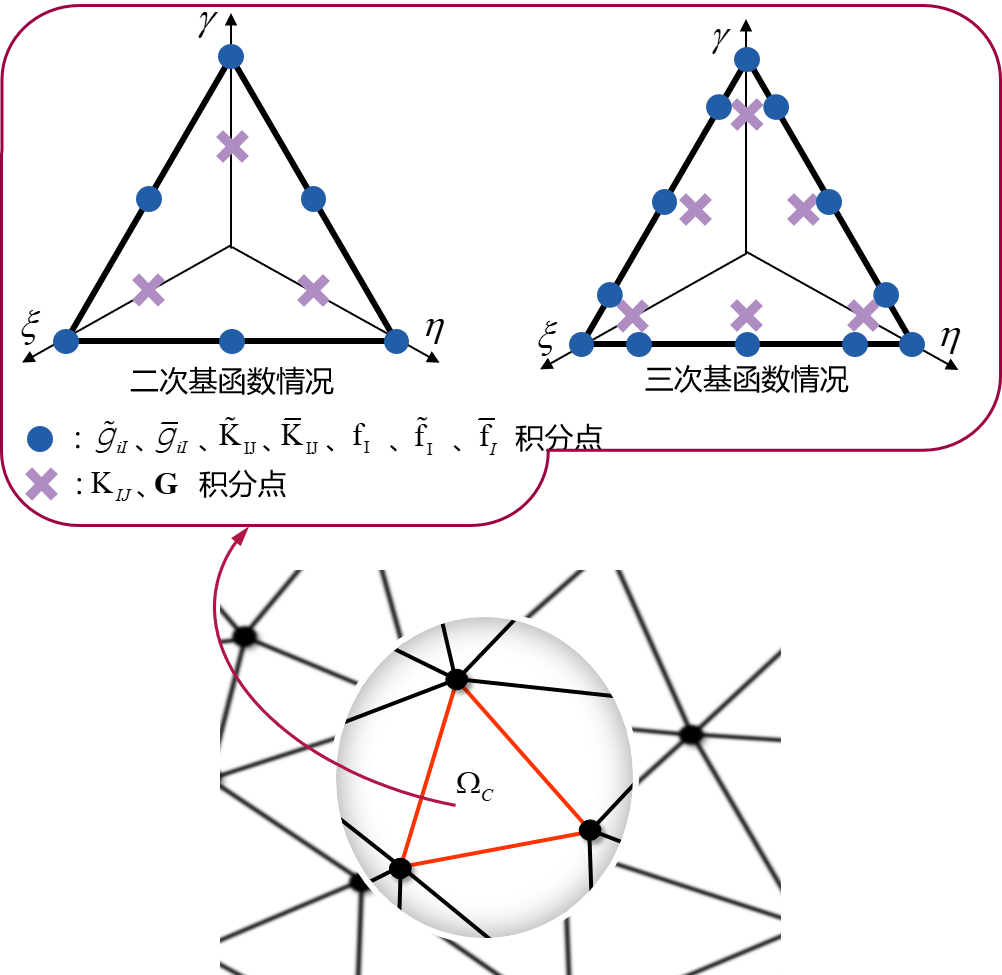
\includegraphics[scale=0.6]{figure/EHR/Eintegralscheme.png}
    \caption{优化的数值积分方案}\label{Eintegralscheme}
\end{figure}
基于赫林格-赖斯纳变分原理的本质边界条件施加方法中,再生光滑梯度的构造过程需要计算积分点处的无网格形函数,此时为了减少形函数的计算量提高计算效率,采用无网格再生核光滑梯度积分法。
无网格再生核光滑梯度积分法利用积分点在背景积分单元间的共享特性,优化整体求解数值过程中积分点的数量,从而提高计算效率。
再生核光滑梯度积分法通过在背景积分单元上选择合适的积分点分布,使得积分点在不同单元之间共享,减少需要计算的积分点数量,进而保证计算精度的前提下进一步提高计算效率,
具体的数值积分方案见附录C再生光滑梯度优化的数值积分方案。
\section{数值算例}
\subsection{分片实验}
首先采用线性、二次和三次弹性力学分片实验验证采用传统高斯积分法和再生光滑梯度积分法的不同本质边界条件施加方法下是否满足积分约束条件的情况。
分片实验考虑求解域为边长等于1的正方形,求解域正方形的四边施加本质边界条件。其分片实验的精确解如下:
\begin{equation}
\begin{split}
    \begin{cases}
        u_x(x,y)=(1+2x+3y)^n\\
        u_y(x,y)=(4+5x+6y)^n
    \end{cases}
\end{split}
\end{equation}
其中,$n=1,2,3$表示线性、二次和三次分片实验。如图\ref{patchtestmeshfree}所示,分片实验采用$11\times 11$的非均匀节点离散求解域。针对二次基函数的无网格近似,分别采用线性和二次分片实验进行测试,核函数相对影响域在二次基函数情况下为2.5;
三次基函数的无网格近似则分别采用二次和三次分片实验进行测试,核函数相对影响域在三次基函数情况下为3.5。\par
分别采用位移误差$L_2$-Error和能量误差$H_1$-Error详细对比所提方法的计算精度
\begin{equation}
\begin{split}
    L_2\text{-Error}=\sqrt{\int_{\Omega}(u_i-u_i^h)(u_i-u_i^h)d\Omega}
\end{split}
\end{equation}
\begin{equation}
    \begin{split}
        H_1\text{-Error}=\sqrt{\frac{1}{2}\int_{\Omega}(\sigma_{ij}-\sigma_{ij}^h)C_{ijkl}^{-1}(\sigma_{ij}-\sigma_{ij}^h)d\Omega}
    \end{split}
    \end{equation}\par
\begin{figure}[H]
    \centering
    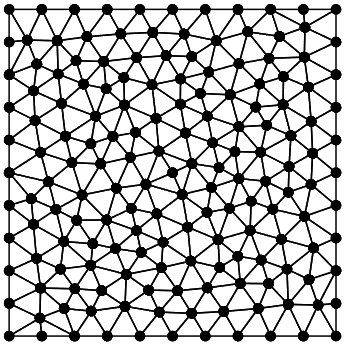
\includegraphics[scale=0.7]{figure/EHR/patchtestmeshfree.png}
    \caption{分片实验无网格离散模型}\label{patchtestmeshfree}
\end{figure} 
在数值结果中,“GI”表示采用的是传统高斯积分法,“RKGSI”表示采用的是再生光滑梯度积分法。“Penalty”、“LM”和“Nitsche”分别表示罚函数法、拉格朗日乘子法和Nitsche法三种常见的本质边界条件施加方法。“RKGSI-HR”则表示的是本章提出的
基于赫林格-赖斯纳变分原理的本质边界条件施加方法。\par
在数值求解过程中,为了保证拉格朗日乘子法的稳定性,拉格朗日乘子统一采用线性有限元形函数进行离散。针对二次基函数的求解,高斯积分法“GI”的求解域$\Omega$的积分采用13点高斯积分点,边界$\Gamma$积分则采用3点高斯积分点
;针对三次基函数的求解,高斯积分法“GI”的求解域$\Omega$的积分采用16点高斯积分点,边界$\Gamma$积分采用5点高斯积分点。采用二次和三次基函数的无网格法分片试验结果如下:\par
\begin{table}[H]
\caption{\textbf{二次基函数无网格法分片实验结果}}
\centering\label{EEquadratic}
\begin{tabular}{lcccc}
   \toprule
& \multicolumn{2}{c}{线性分片实验} & \multicolumn{2}{c}{二次分片实验} \\ \cline{2-5}
   &$L_2$-Error$\quad$&$H_1$-Error&$L_2$-Error$\quad$&$H_1$-Error\\
   \midrule
   GI-Penalty&$7.7\times10^{-6}$&$2.7\times10^{-4}$&$1.2\times10^{-5}$&$2.6\times10^{-4}$\\
   GI-LM&$1.0\times10^{-4}$&$4.7\times10^{-3}$&$1.5\times10^{-4}$&$4.3\times10^{-3}$\\
   GI-Nitsche&$8.1\times10^{-6}$&$2.8\times10^{-4}$&$1.3\times10^{-5}$&$2.8\times10^{-4}$\\
  RKGSI-Penalty&$7.9\times10^{-8}$&$2.0\times10^{-6}$&$1.4\times10^{-7}$&$2.1\times10^{-6}$\\
  RKGSI-LM&$8.6\times10^{-5}$&$4.0\times10^{-3}$&$1.4\times10^{-4}$&$3.7\times10^{-3}$\\
  RKGSI-Nitsche&$2.1\times10^{-15}$&$4.0\times10^{-14}$&$2.2\times10^{-15}$&$2.7\times10^{-14}$\\
  RKGSI-HR&$2.0\times10^{-15}$&$3.2\times10^{-14}$&$2.2\times10^{-15}$&$2.1\times10^{-14}$\\
\bottomrule
\end{tabular}
\end{table}
\begin{table}[H]
\caption{\textbf{三次基函数无网格法分片实验结果}}
\centering\label{EEcubic}
\begin{tabular}{lcccc}
   \toprule
& \multicolumn{2}{c}{二次分片实验} & \multicolumn{2}{c}{三次分片实验} \\ \cline{2-5}
   &$L_2$-Error$\quad$&$H_1$-Error&$L_2$-Error$\quad$&$H_1$-Error\\
   \midrule
   GI-Penalty&$9.1\times10^{-6}$&$2.1\times10^{-4}$&$1.2\times10^{-5}$&$2.0\times10^{-4}$\\
   GI-LM&$2.9\times10^{-4}$&$9.3\times10^{-3}$&$4.0\times10^{-4}$&$9.3\times10^{-3}$\\
   GI-Nitsche&$1.1\times10^{-5}$&$2.8\times10^{-4}$&$1.4\times10^{-5}$&$2.7\times10^{-4}$\\
  RKGSI-Penalty&$1.4\times10^{-7}$&$2.1\times10^{-6}$&$2.0\times10^{-7}$&$2.7\times10^{-6}$\\
  RKGSI-LM&$3.0\times10^{-4}$&$9.8\times10^{-3}$&$4.2\times10^{-4}$&$9.8\times10^{-3}$\\
  RKGSI-Nitsche&$3.6\times10^{-15}$&$1.0\times10^{-13}$&$4.6\times10^{-15}$&$9.5\times10^{-14}$\\
  RKGSI-HR&$3.1\times10^{-15}$&$1.0\times10^{-13}$&$3.5\times10^{-15}$&$7.4\times10^{-14}$\\
   \bottomrule
\end{tabular}
\end{table}
表\ref{EEquadratic}和表\ref{EEcubic}分别为具有二次、三次基函数无网格法的分片试验结果,
从表中可以看出,由于传统高斯积分法不满足积分约束条件,所以即使采用高阶高斯积分的罚函数法“GI-Penalty”、拉格朗日乘子法“GI-LM”和Nitsche法“GI-Nitsche”均不能通过分片试验。
当采用满足积分约束条件的再生光滑梯度积分法时,此时由于罚函数法“RKGSI-Penalty”不具有变分一致性,也无法通过分片试验;
拉格朗日乘子法“RKGSI-LM”由于其拉格朗日乘子采用线性形函数进行离散,无法与再生光滑梯度相匹配,也无法通过分片试验;
当采用Nitsche法“RKGSI-Nitsche”和基于赫林格-赖斯纳变分原理“RKGSI-HR”的本质边界条件施加方法时,均可以通过分片试验,即满足积分约束条件。
\subsection{悬臂梁问题}
首先考虑经典弹性力学二维悬臂梁问题,如图\ref{cantilever}所示,悬臂梁的长和宽分别为$L=48$,$D=12$,同时悬臂梁的左端为固定支座,
右端沿着$y$轴正方向施加外部荷载$P=1000$。悬臂梁的材料系数为杨氏模量$E=3\times10^6$、泊松比$\nu=0.3$。
根据圣维南原理和平面应力假设,悬臂梁问题的解析解为:
\begin{equation}
\begin{split}
\begin{cases}
    u = -\frac{Py}{6EI}[(6L-3x)x + (2+\nu)(y^2 - \frac{D^2}{4})] \\
    v = \frac{P}{6EI}[3\nu y^2(L-x) + (4+5\nu)\frac{D^2x}{4} + (3L-x)x^2]
\end{cases}
\end{split}
\end{equation}
与之相对应的应力分量为:
\begin{equation}
\begin{split}
\begin{cases}
   \sigma_{xx}=-\frac{P(L-x)y}{I}\\
   \sigma_{yy}=0\\
   \sigma_{xy}=\frac{P}{2I}(\frac{D^2}{4}-y^2)
\end{cases}
\end{split}
\end{equation}
\begin{figure}[H]
    \centering
    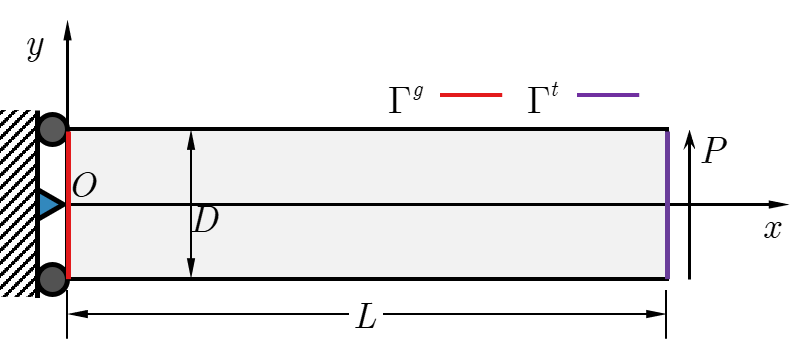
\includegraphics[scale=0.7]{figure/EHR/cantilever/cantilever.png}
    \caption{悬臂梁问题模型}\label{cantilever}
\end{figure}
如图\ref{cantilever}所示,悬臂梁的左端施加自然边界条件$\Gamma^t$,右端施加本质边界条件$\Gamma^g$。
悬臂梁求解域分别通过图\ref{cantilever.mesh}所示采用四个疏密不同的节点进行离散。对于采用二次基函数的悬臂梁算例问题,传统高斯积分法采用13点高斯积分,核函数的相对影响域为2.5。
\newpage
\begin{figure}[H]
    \centering
    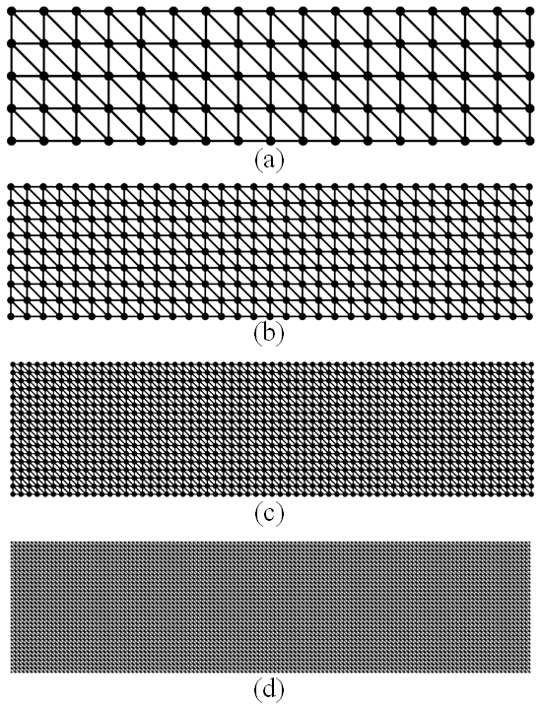
\includegraphics[scale=0.8]{figure/EHR/cantilever/cantilever.mesh.png}
    \caption{悬臂梁问题节点模型}\label{cantilever.mesh}
\end{figure}
图\ref{ECLH}为悬臂梁问题的位移误差和能量误差对比图。从图中可以看出采用再生光滑梯度积分法“RKGSI”的本质边界条件施加方法的计算精度优于采用高斯积分法“GI”的本质条件施加方法,
并且由于传统高斯积分法和采用再生光滑梯度积分法的罚函数法“RKGSI-Penalty”和拉格朗日乘子法“RKGSI-LM”不具有变分一致性,无法达到理论误差收敛率,而基于赫林格-赖斯纳变分原理下的本质边界条件施加方法“RKGSI-HR”和Nitshce法“RKGSI-Nitsche”均可达到理论误差收敛率,但相较于“RKGSI-Nitsche”法,所提出的“RKGSI-HR”法无需引入人工参数。
\par
图\ref{ECcputime}为悬臂梁问题的节点数和计算时间的效率对比和本质边界条件施加效率对比图。从整体来看采用传统高斯积分法“GI”的计算效率明显低于再生光滑梯度积分法“RKGSI”,耗时高于再生光滑梯度积分法。
图\ref{ECefficiency}为悬臂梁问题的本质边界条件施加效率分析对比图。该图为施加本质边界$\Gamma^g$过程中计算形函数及梯度和组装相对应的刚度矩阵和力向量所用时间对比图。
由图可知,罚函数法和拉格朗日乘子法在计算形函数及其梯度这部分所用的时间相同且所用时间最少,这是由于罚函数法和拉格朗日乘子法在数值计算过程中只需要计算无网格形函数本身,无需计算无网格形函数梯度,
而“RKGSI-HR”法也无需计算无网格形函数梯度,但需要计算再生光滑梯度,“RKGSI-Nitsche”法这部分所用的时间是罚函数法和拉格朗日乘子法的5.6倍,而“RKGSI-HR”法是1.6倍,“RKGSI-HR”法的计算效率高于“RKGSI-Nitsche”法。
组装相应的刚度矩阵和力向量这部分所用的时间上,“RKGSI-Nitsche”法和“RKGSI-HR”法计算效率基本相同。
从整体上来看,拉格朗日乘子法和罚函数法的效率优于“HR”法和“Nitsche”法,但拉格朗日乘子法和罚函数法不满足变分一致性无法达到理论误差收敛率。
因此,总体来说,相较于传统的本质边界条件施加方法,基于赫林格-赖斯纳变分原理的本质边界条件施加方法“RKGSI-HR”能够达到理论误差收敛率,有效提高计算精度,相较于“RKGSI-Nitsche”法而言计算效率也更高。
\begin{figure}[H]
\centering
\begin{subcaptiongroup}
    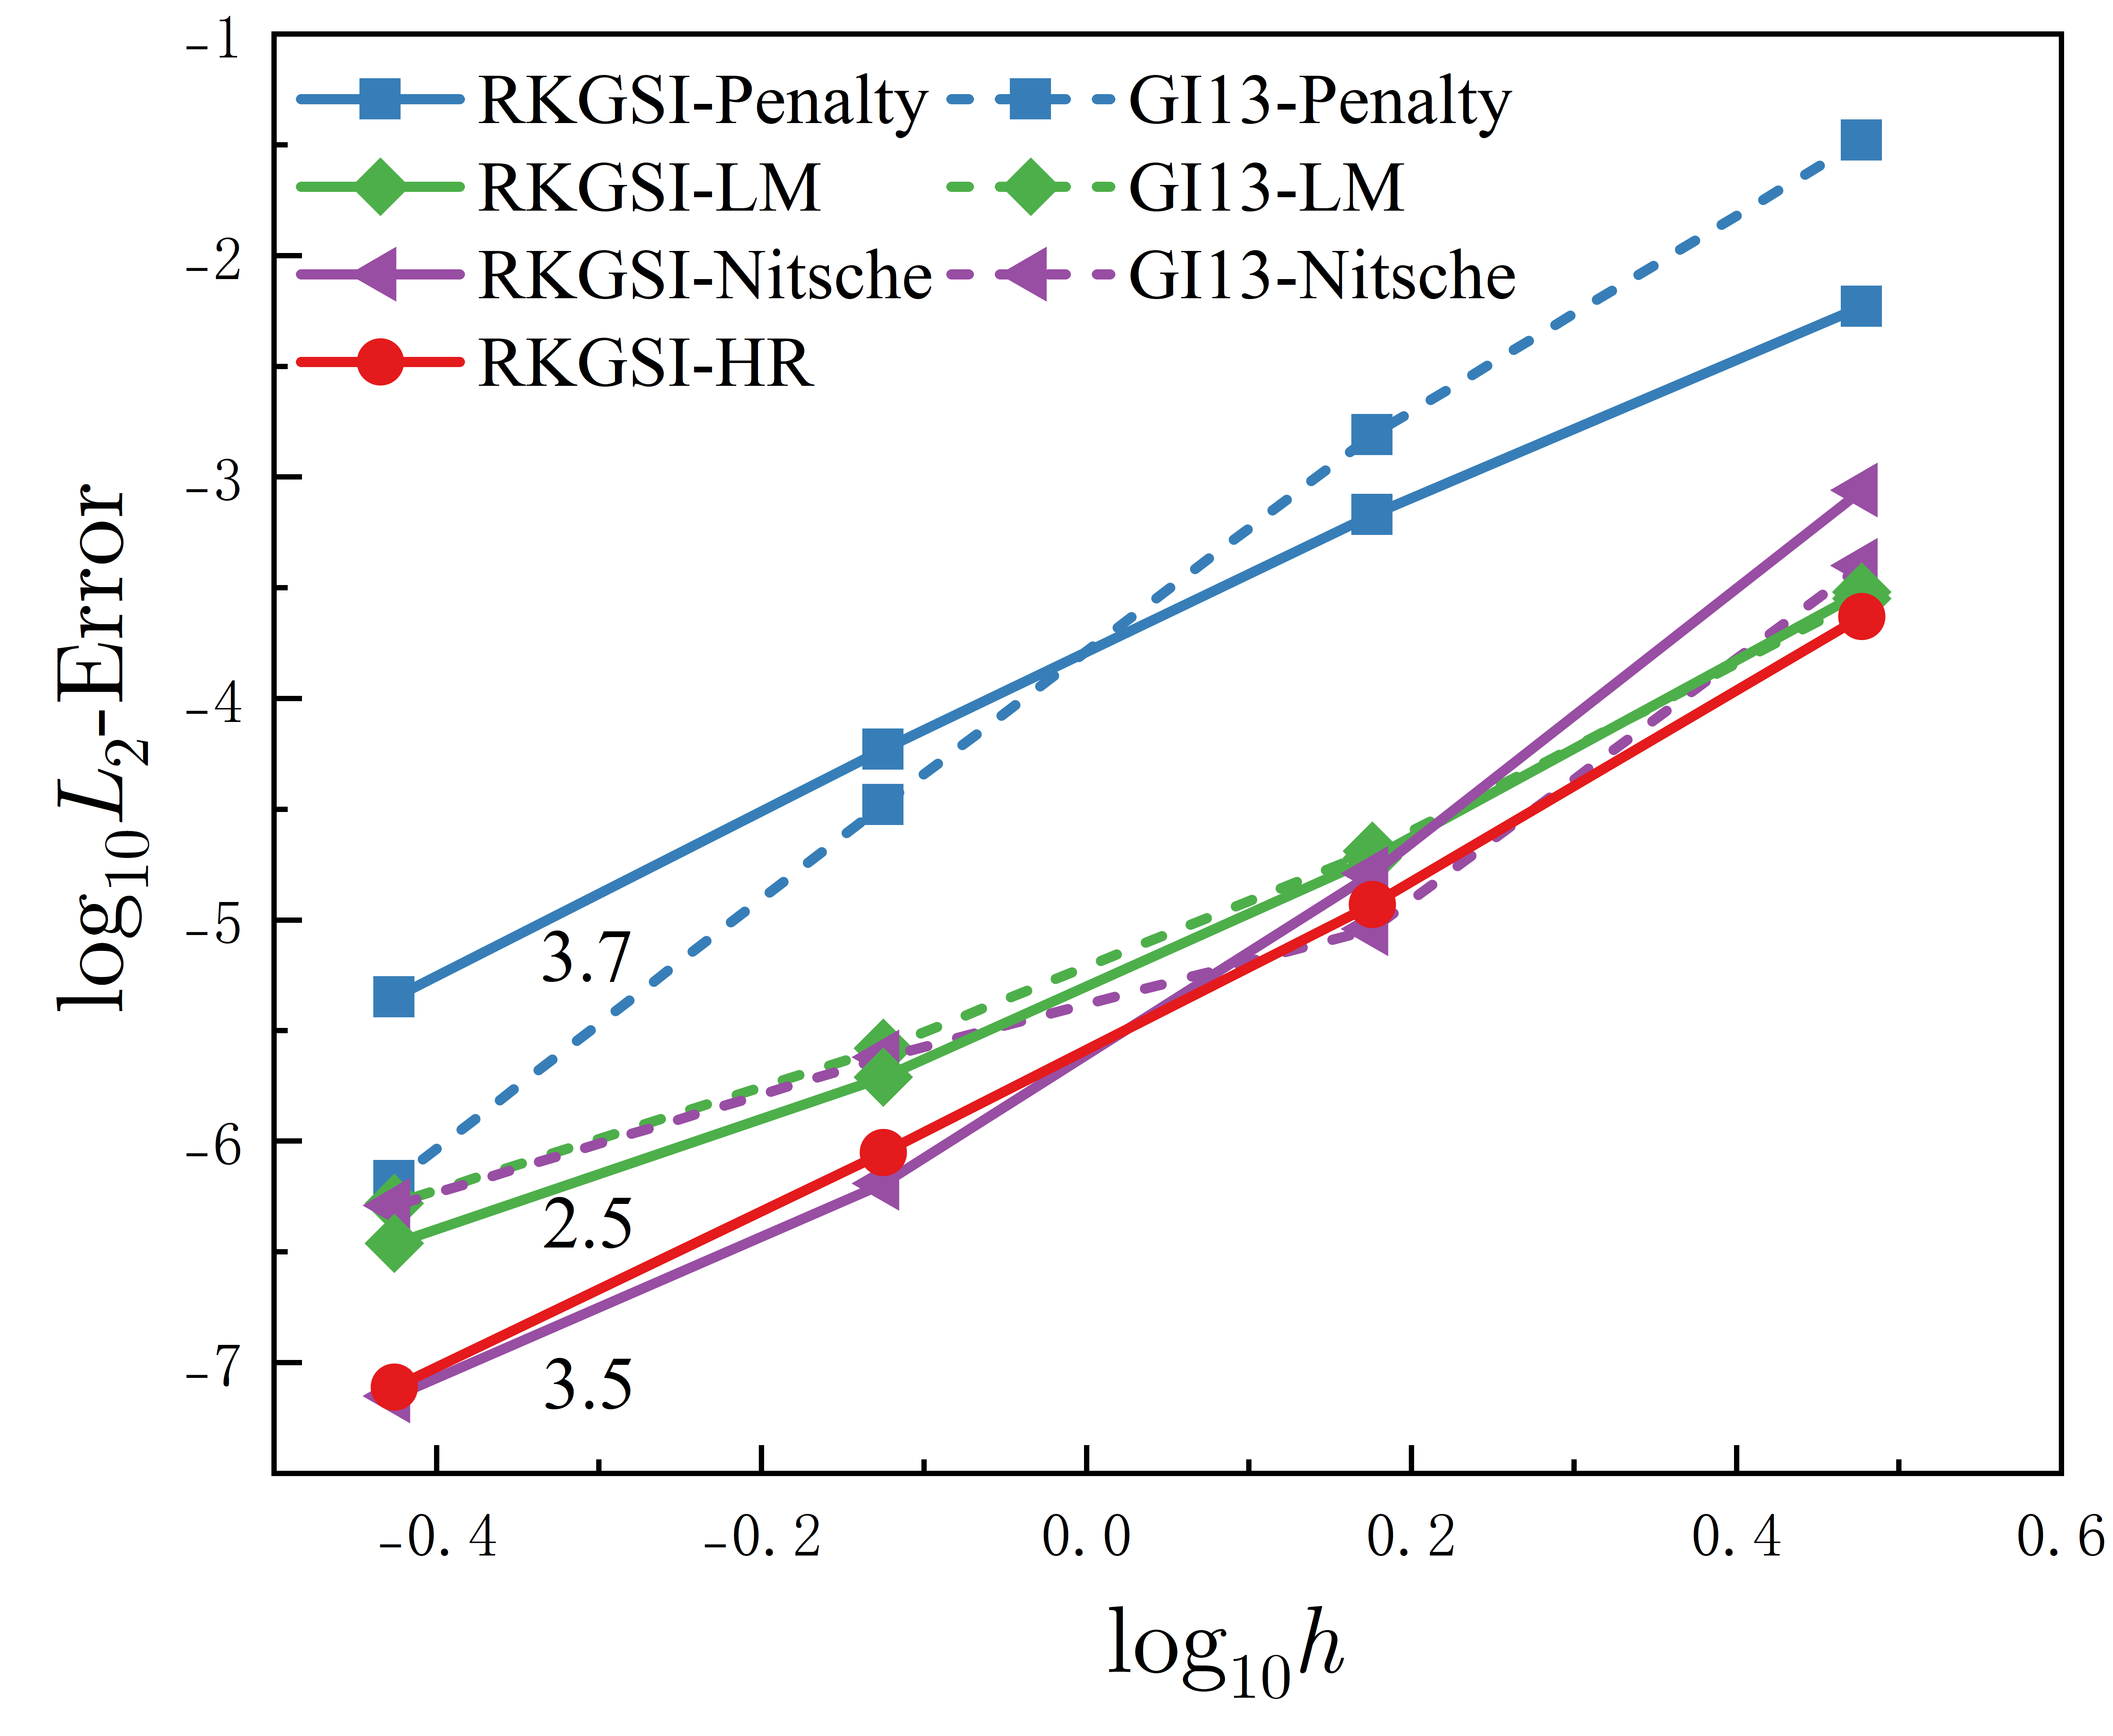
\includegraphics[width=0.49\textwidth]{figure/EHR/cantilever/L2.png}
    \phantomcaption\label{ECL2}
    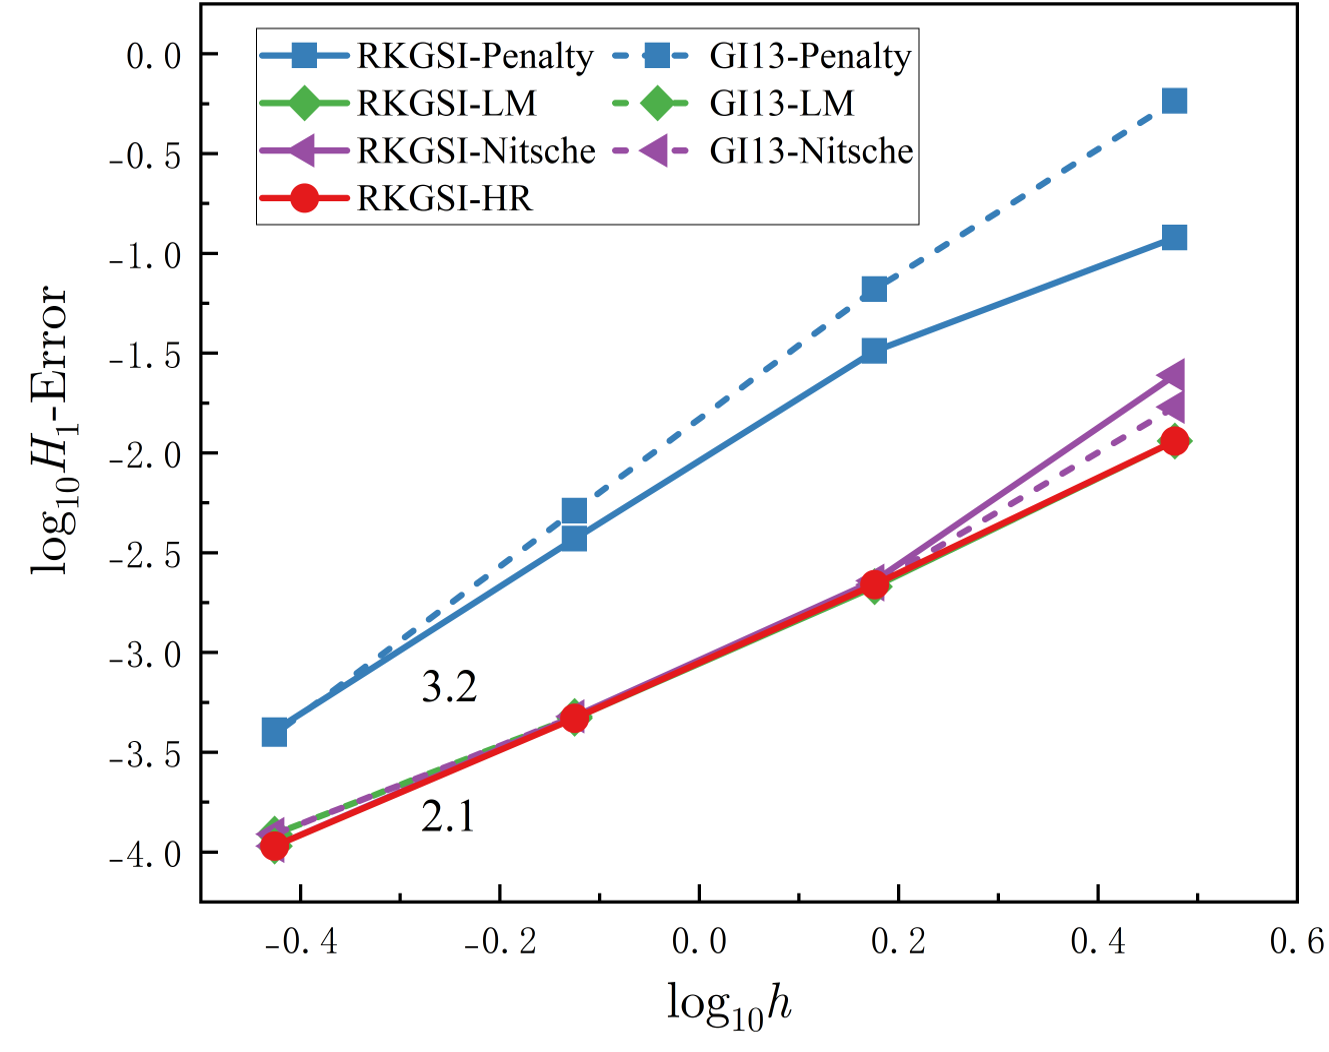
\includegraphics[width=0.49\textwidth]{figure/EHR/cantilever/H1.png}
    \phantomcaption\label{ECH1}
    \end{subcaptiongroup}
\caption{悬臂梁问题误差对比:\subref{ECL2} $L_2$误差;\subref{ECH1} $H_1$误差}
\label{ECLH}
\end{figure}
\begin{figure}[H]
\centering
    \begin{subcaptiongroup}
        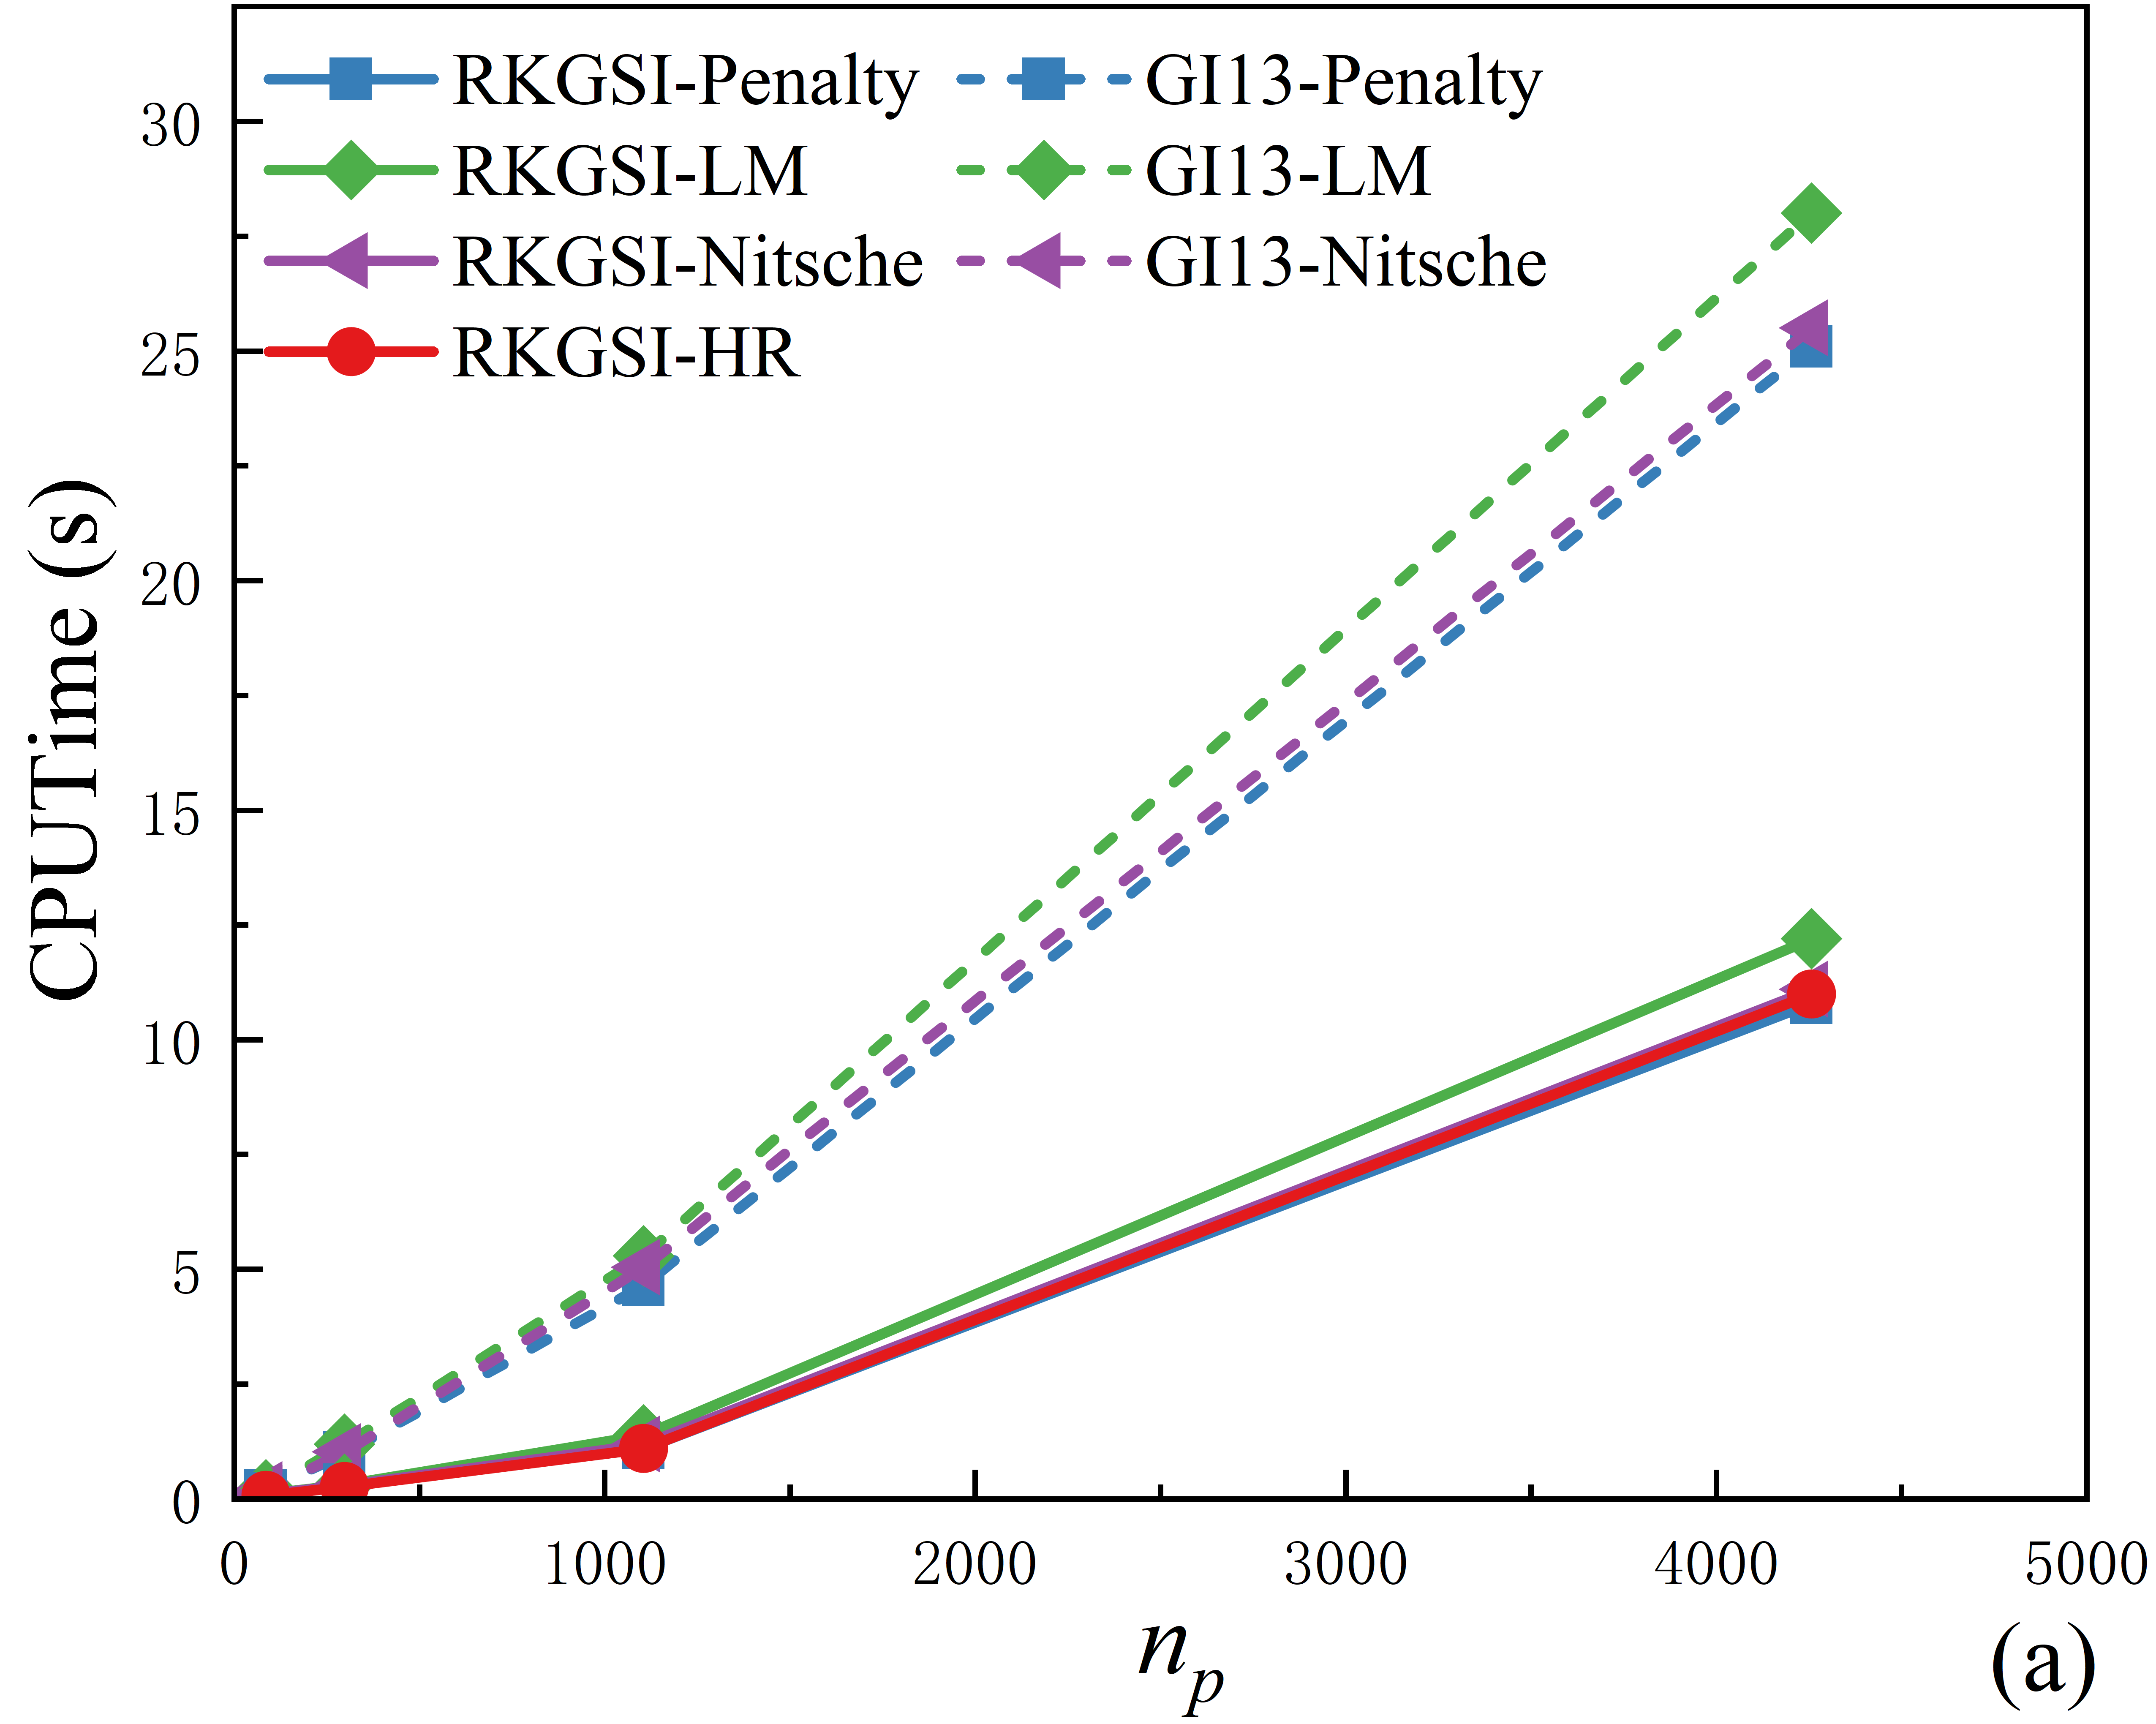
\includegraphics[width=0.49\textwidth]{figure/EHR/cantilever/cputime.png}
        \phantomcaption\label{ECcputime}
        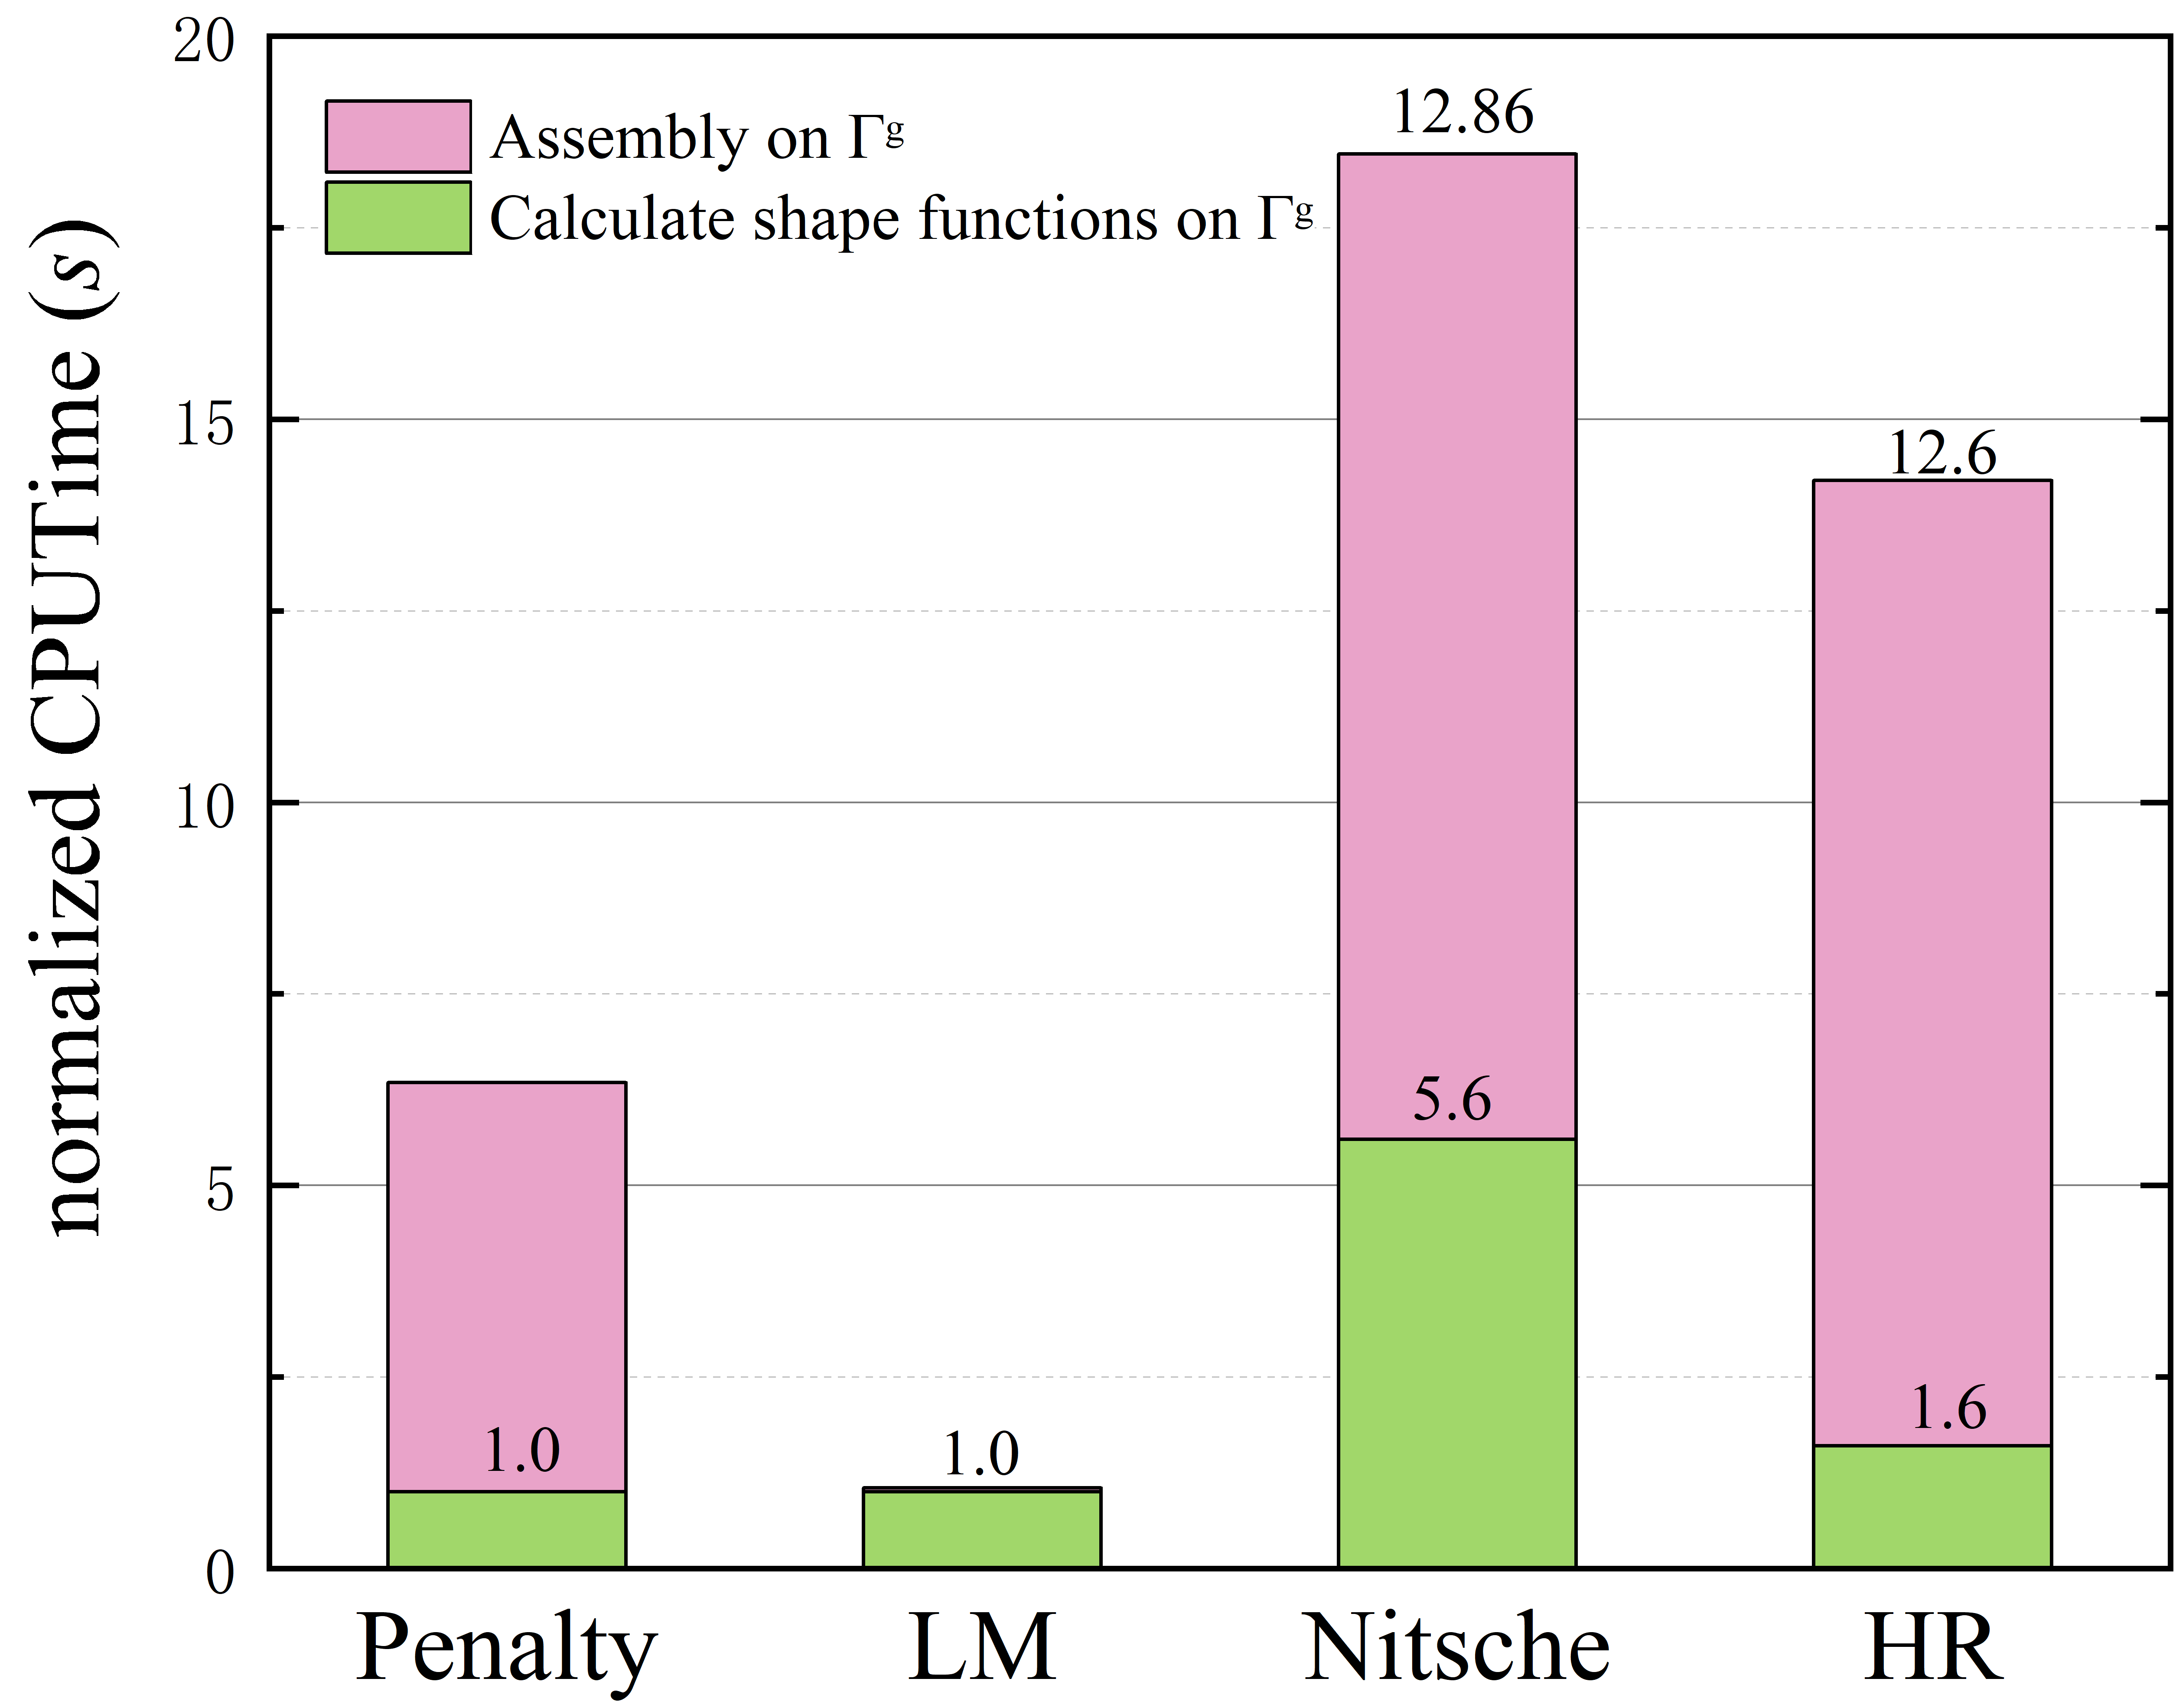
\includegraphics[width=0.49\textwidth]{figure/EHR/cantilever/efficiency.png}
        \phantomcaption\label{ECefficiency}
        \end{subcaptiongroup}
\caption{悬臂梁问题效率对比:\subref{ECcputime} 计算时间与节点数的关系;\subref{ECefficiency} 边界条件施加效率分析}
\end{figure}
\subsection{带孔无限大平板问题}
考虑经典的带孔无限大平板问题,如图\ref{hole}所示,板的的中心存在一半径为$a=1$的圆形小孔,同时平板的无穷远处沿$x$轴方向施加均布荷载$T=1000$。
板的材料系数为杨氏模量$E=3\times10^6$、泊松比$\nu=0.3$。根据Michell解可以得到该带孔无限大平板问题的解析解为:
\begin{equation}
\begin{split}
\begin{cases}
    u_x(r,\theta)=\frac{Ta}{8\mu}(\frac{r}{a}(k+1)cos\theta-\frac{2a^3}{r^3}cos3\theta+\frac{2a}{r}((1+k)cos\theta+cos3\theta))\\
    u_y(r,\theta)=\frac{Ta}{8\mu}(\frac{r}{a}(k-3)sin\theta-\frac{2a^3}{r^3}sin3\theta+\frac{2a}{r}((1-k)sin\theta+sin3\theta))  
\end{cases}
\end{split}
\end{equation}
其中,$k$和$\mu$分别为:
\begin{equation}
\begin{split}
    k=\frac{3-\nu}{1+\nu}\quad \text{,}\mu=\frac{E}{2(1+\nu)}
\end{split}
\end{equation}
与之相对应的应力分量为:
\begin{equation}
\begin{split}
\begin{cases}
    \sigma_{xx}=T(1-\frac{a^2}{r^2}(\frac{3}{2}cos2\theta+cos4\theta)+\frac{3a^4}{2r^4}cos4\theta)\\
    \sigma_{yy}=-T(\frac{a^2}{r^2}(\frac{1}{2}cos2\theta-cos4\theta)+\frac{3a^4}{2r^4}cos4\theta)\\
    \sigma_{xy}=-T(\frac{a^2}{r^2}(\frac{1}{2}sin2\theta+sin4\theta)-\frac{3a^4}{2r^4}sin4\theta)\\
\end{cases}
\end{split}
\end{equation}\par
如图\ref{hole}所示,根据带孔无限大平板的对称性,取边长$b=5$的四分之一的方形域作为研究对象。
方形域的上端和右端以及圆孔的边界施加自然边界条件$\Gamma^t$,而方形域的左端和下端约束法向位移,施加本质边界条件$\Gamma^g$。
\begin{figure}[H]
\centering
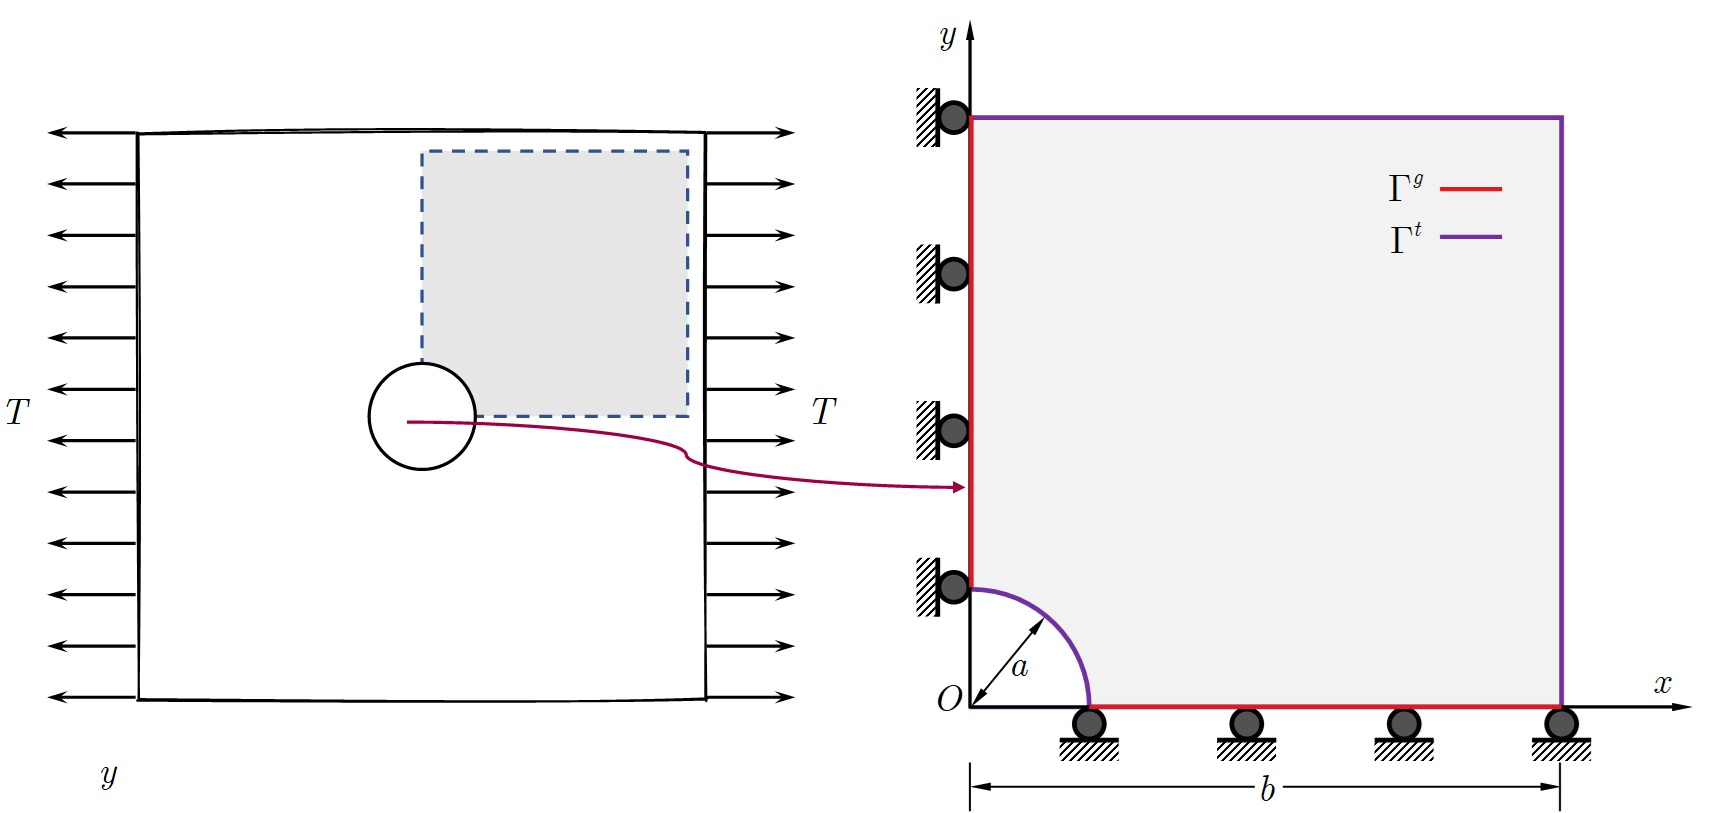
\includegraphics[scale=0.5]{figure/EHR/hole/hole.png}
    \caption{带孔无限大平板问题模型}\label{hole}
\end{figure}
该求解域分别通过图\ref{hole.mesh}所示采用的四个疏密不同的节点进行离散。
对于采用三次基函数的带孔无限大平板算例问题,传统高斯积分法采用16点高斯积分,核函数的相对影响域为3.5。\par
\begin{figure}[H]
\centering
 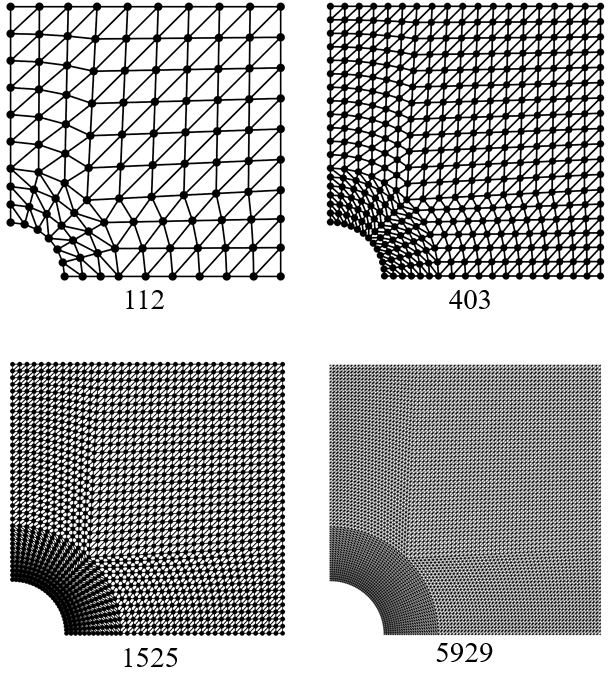
\includegraphics[scale=0.8]{figure/EHR/hole/hole.mesh.png}
   \caption{带孔无限大平板问题无网格离散}\label{hole.mesh}
\end{figure}
图\ref{EHLH}为带孔无限大平板问题的位移和能量误差对比图。
从图中可以看出传统高斯积分法由于不具有变分一致性,导致“GI-Penalty”法、“GI-LM”法、“GI-Nitsche”法均无法达到理论误差收敛率。
基于赫林格-赖斯纳变分原理的本质边界条件施加方法“RKGSI-HR”和“RKGSI-Nitsche”法满足变分一致性能够达到理论误差收敛率。
虽然“RKGSI-LM”法无法通过分片实验不满足变分一致性,但由于拉格朗日乘子法具有较高的精度也能达到理论误差收敛率。
图\ref{Hcputime}、\ref{Hefficiency}为带孔无限大平板问题的效率对比图。
从图中可以看出随着无网格节点数的增加,采用再生光滑梯度积分法“RKGSI”的效率明显高于传统高斯积分法“GI”,在施加本质边界条件的过程中,“HR”法不仅满足变分一致性同时计算效率还高于传统的“Nitsche”法。
最后,图\ref{sigmaxx}为带孔无限大平板问题的应力云图,从图中可以看出“RKGSI-Penalty”法和精确解之间是有差异的,
而“RKGSI-Nitsche”法和“RKGSI-HR”法是和精确解几乎相同。但“Nitsche”法是需要依靠人工经验参数并且计算效率也低于“HR”法。
\newpage
\begin{figure}[H]
\centering
\begin{subcaptiongroup}
        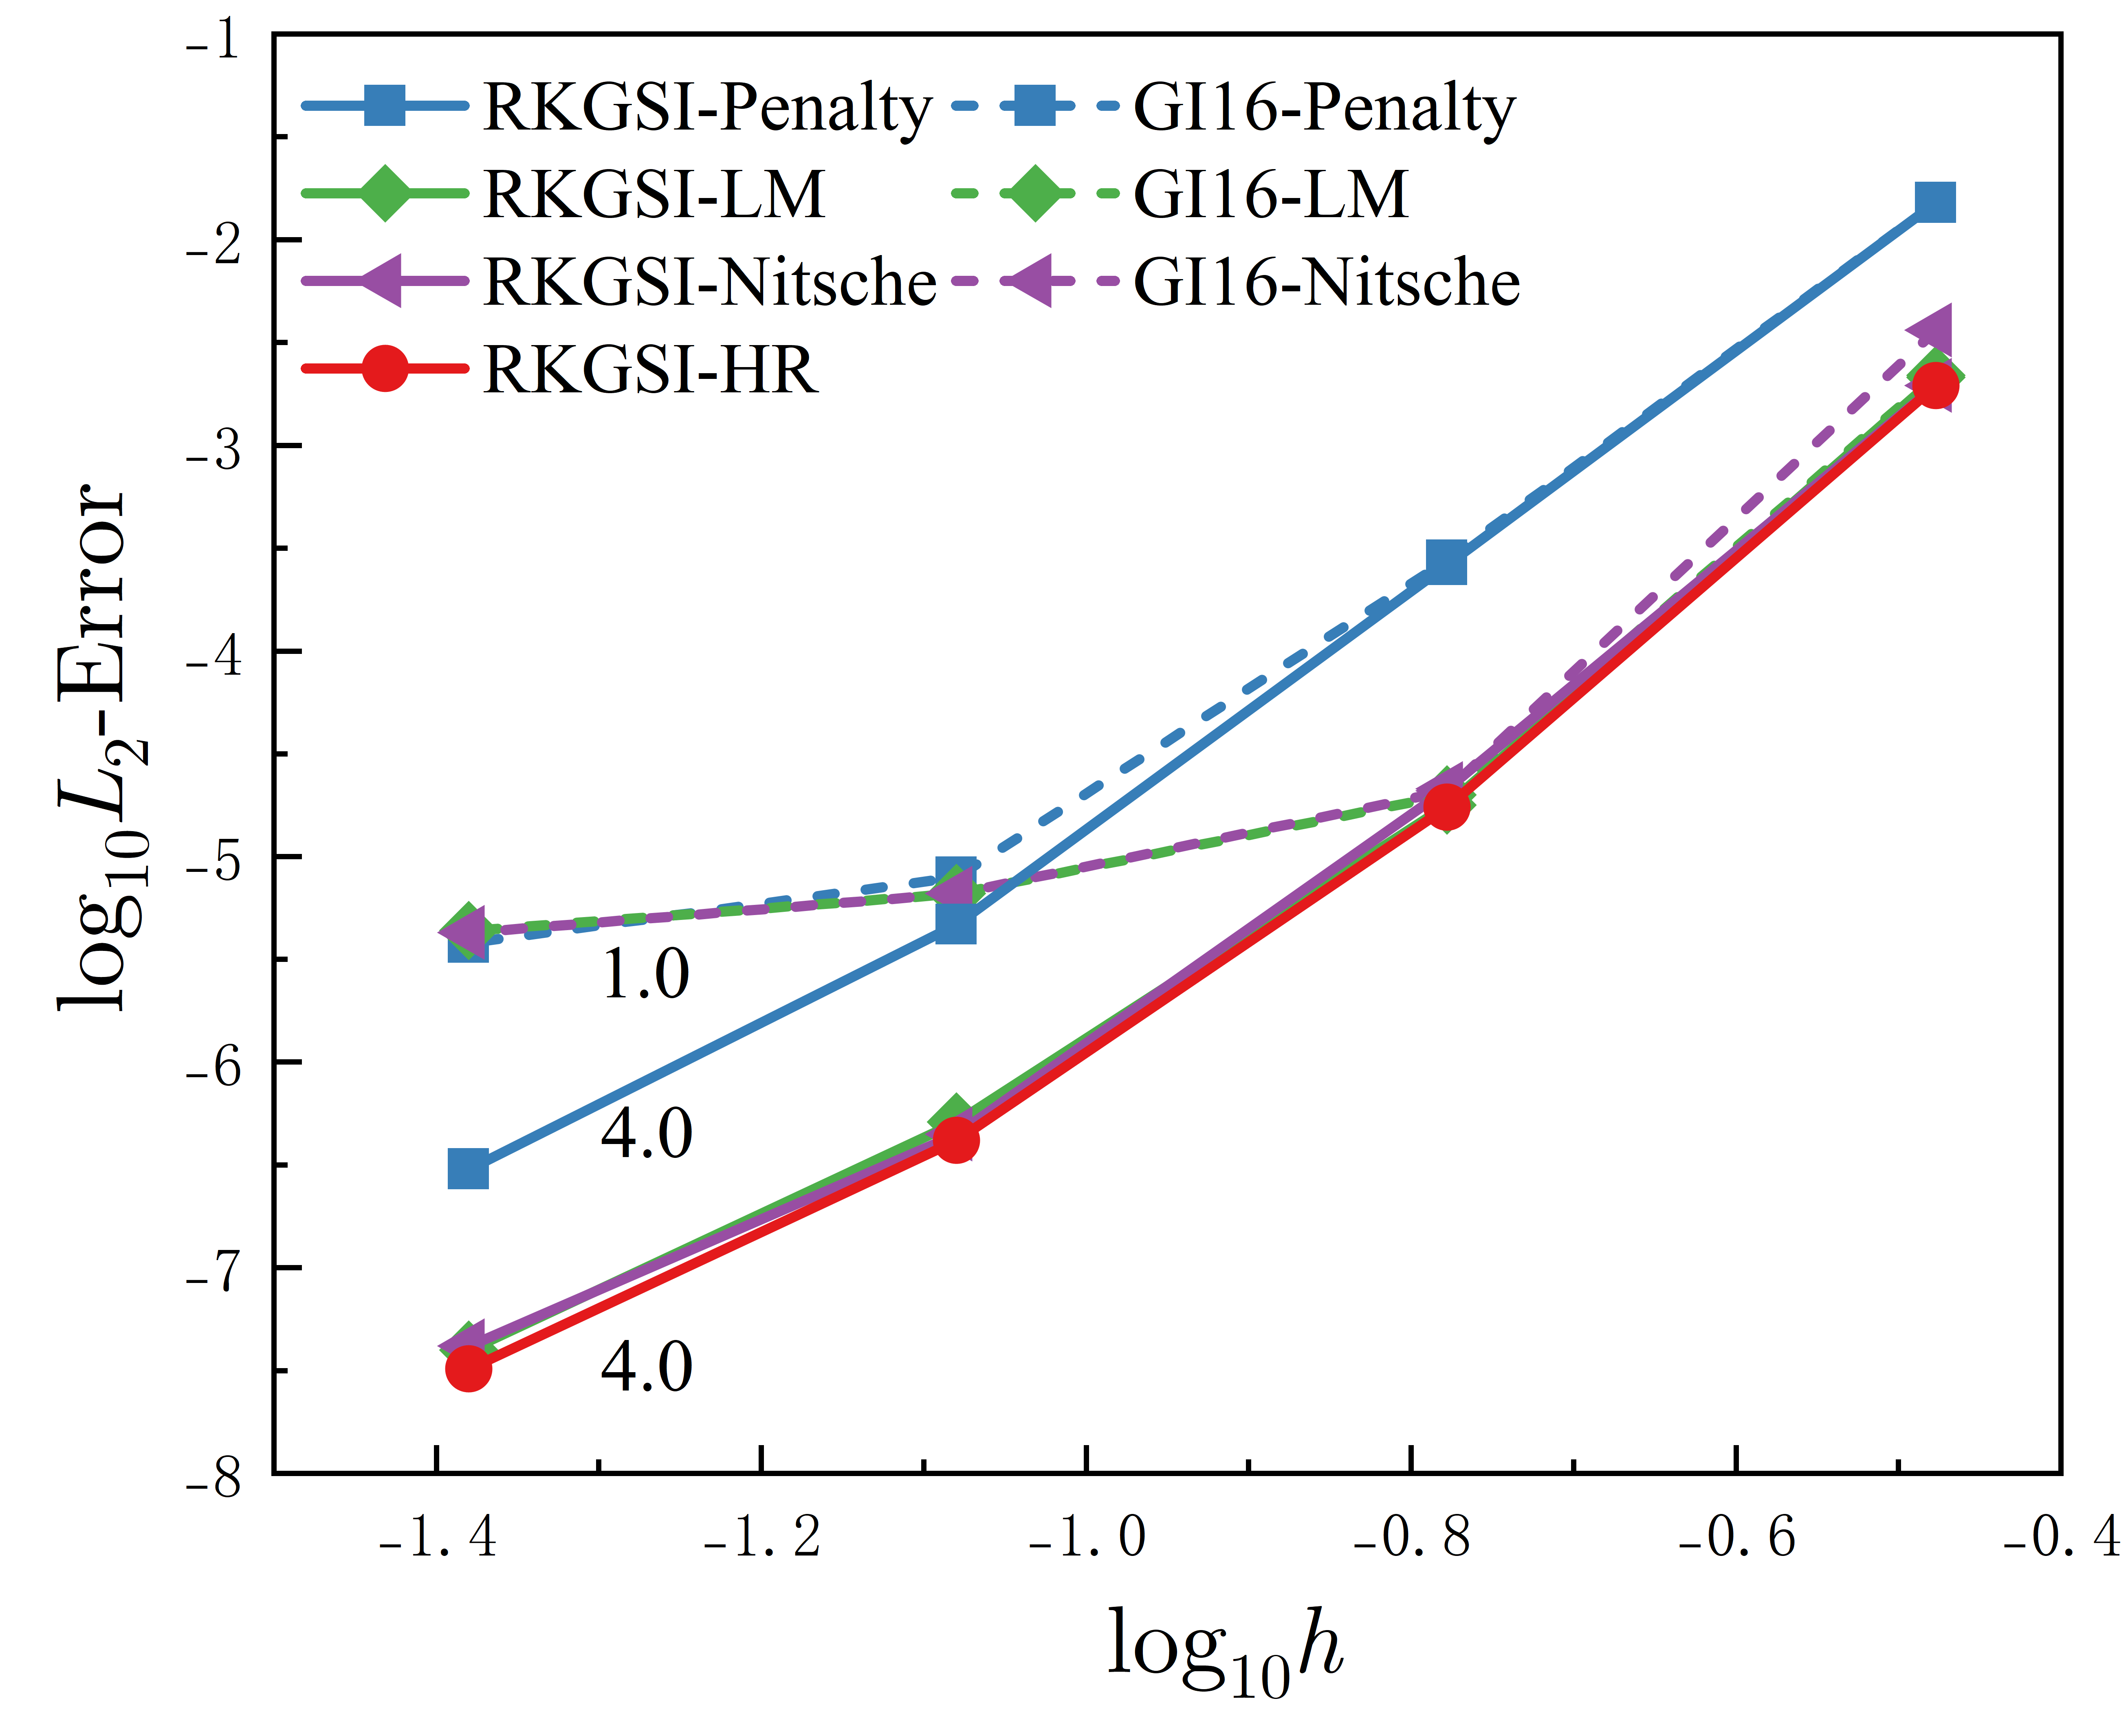
\includegraphics[width=0.49\textwidth]{figure/EHR/hole/L2.png}
        \phantomcaption\label{EHL2}
        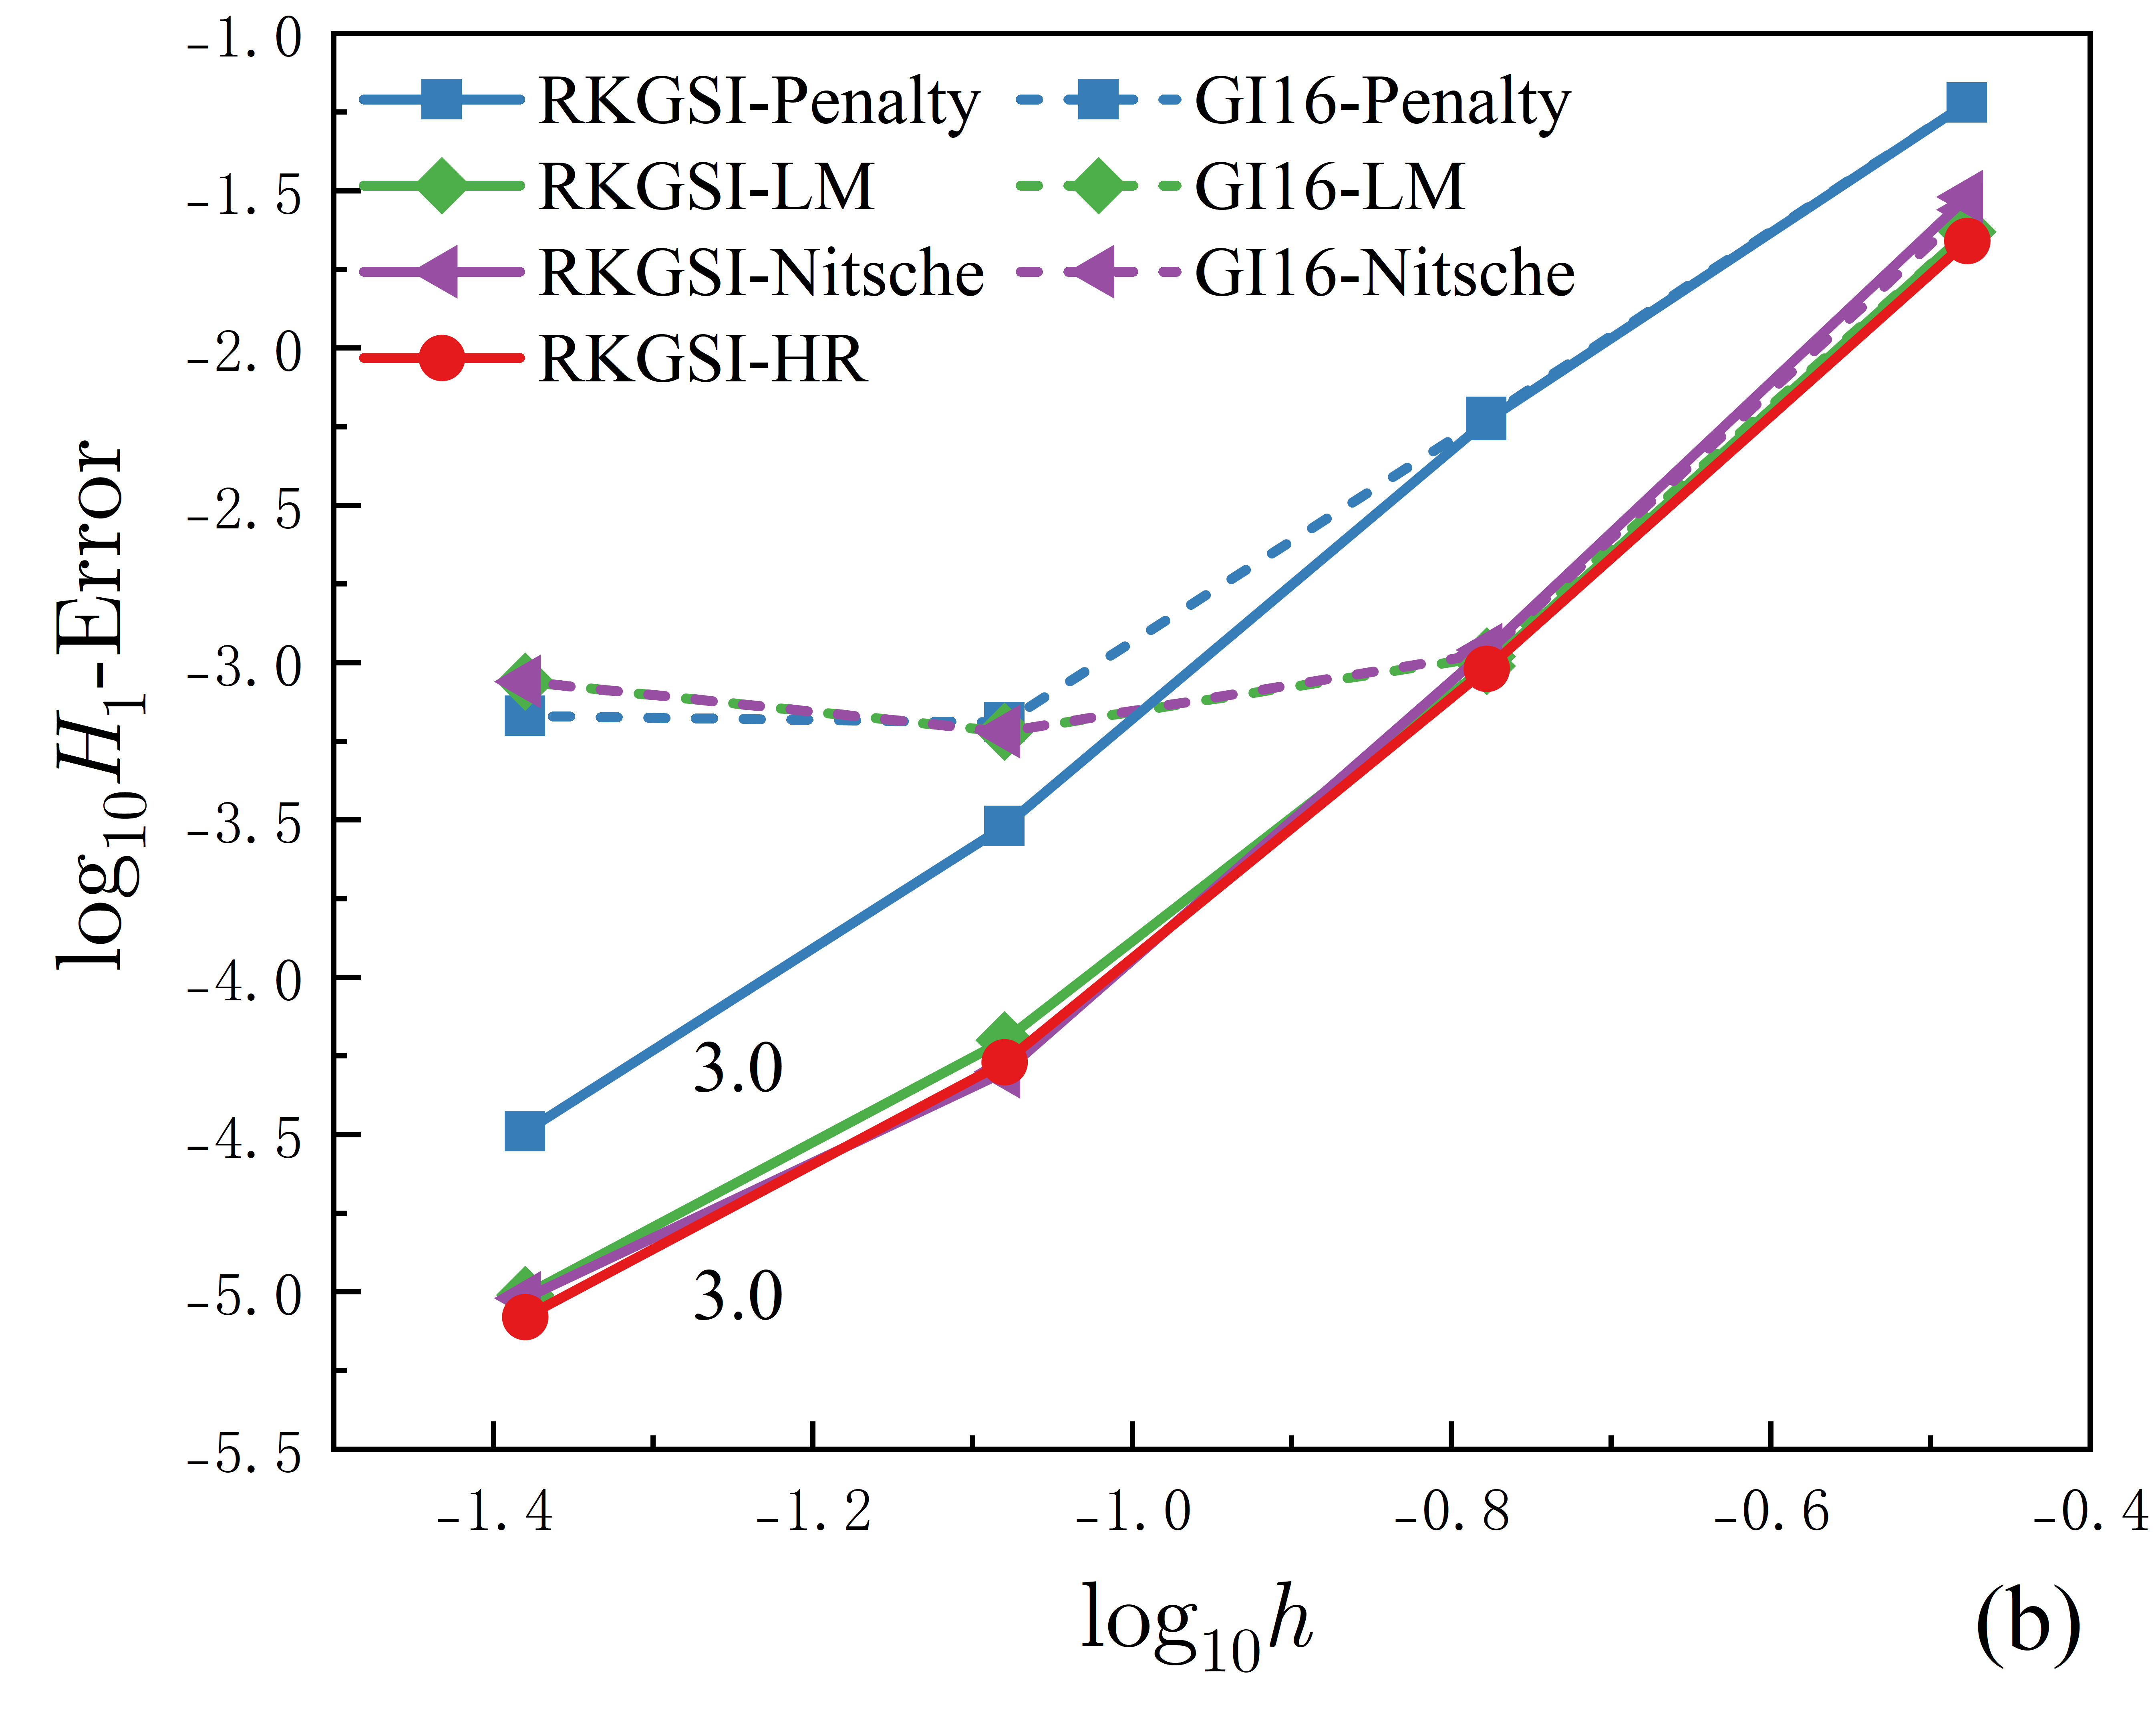
\includegraphics[width=0.49\textwidth]{figure/EHR/hole/H1.png}
        \phantomcaption\label{EHH1}
        \end{subcaptiongroup}
    \caption{带孔无限大平板问题误差对比:\subref{EHL2} $L_2$误差;\subref{EHH1} $H_1$误差}
    \label{EHLH}
    \end{figure}
\begin{figure}[H]
\centering
    \begin{subcaptiongroup}
    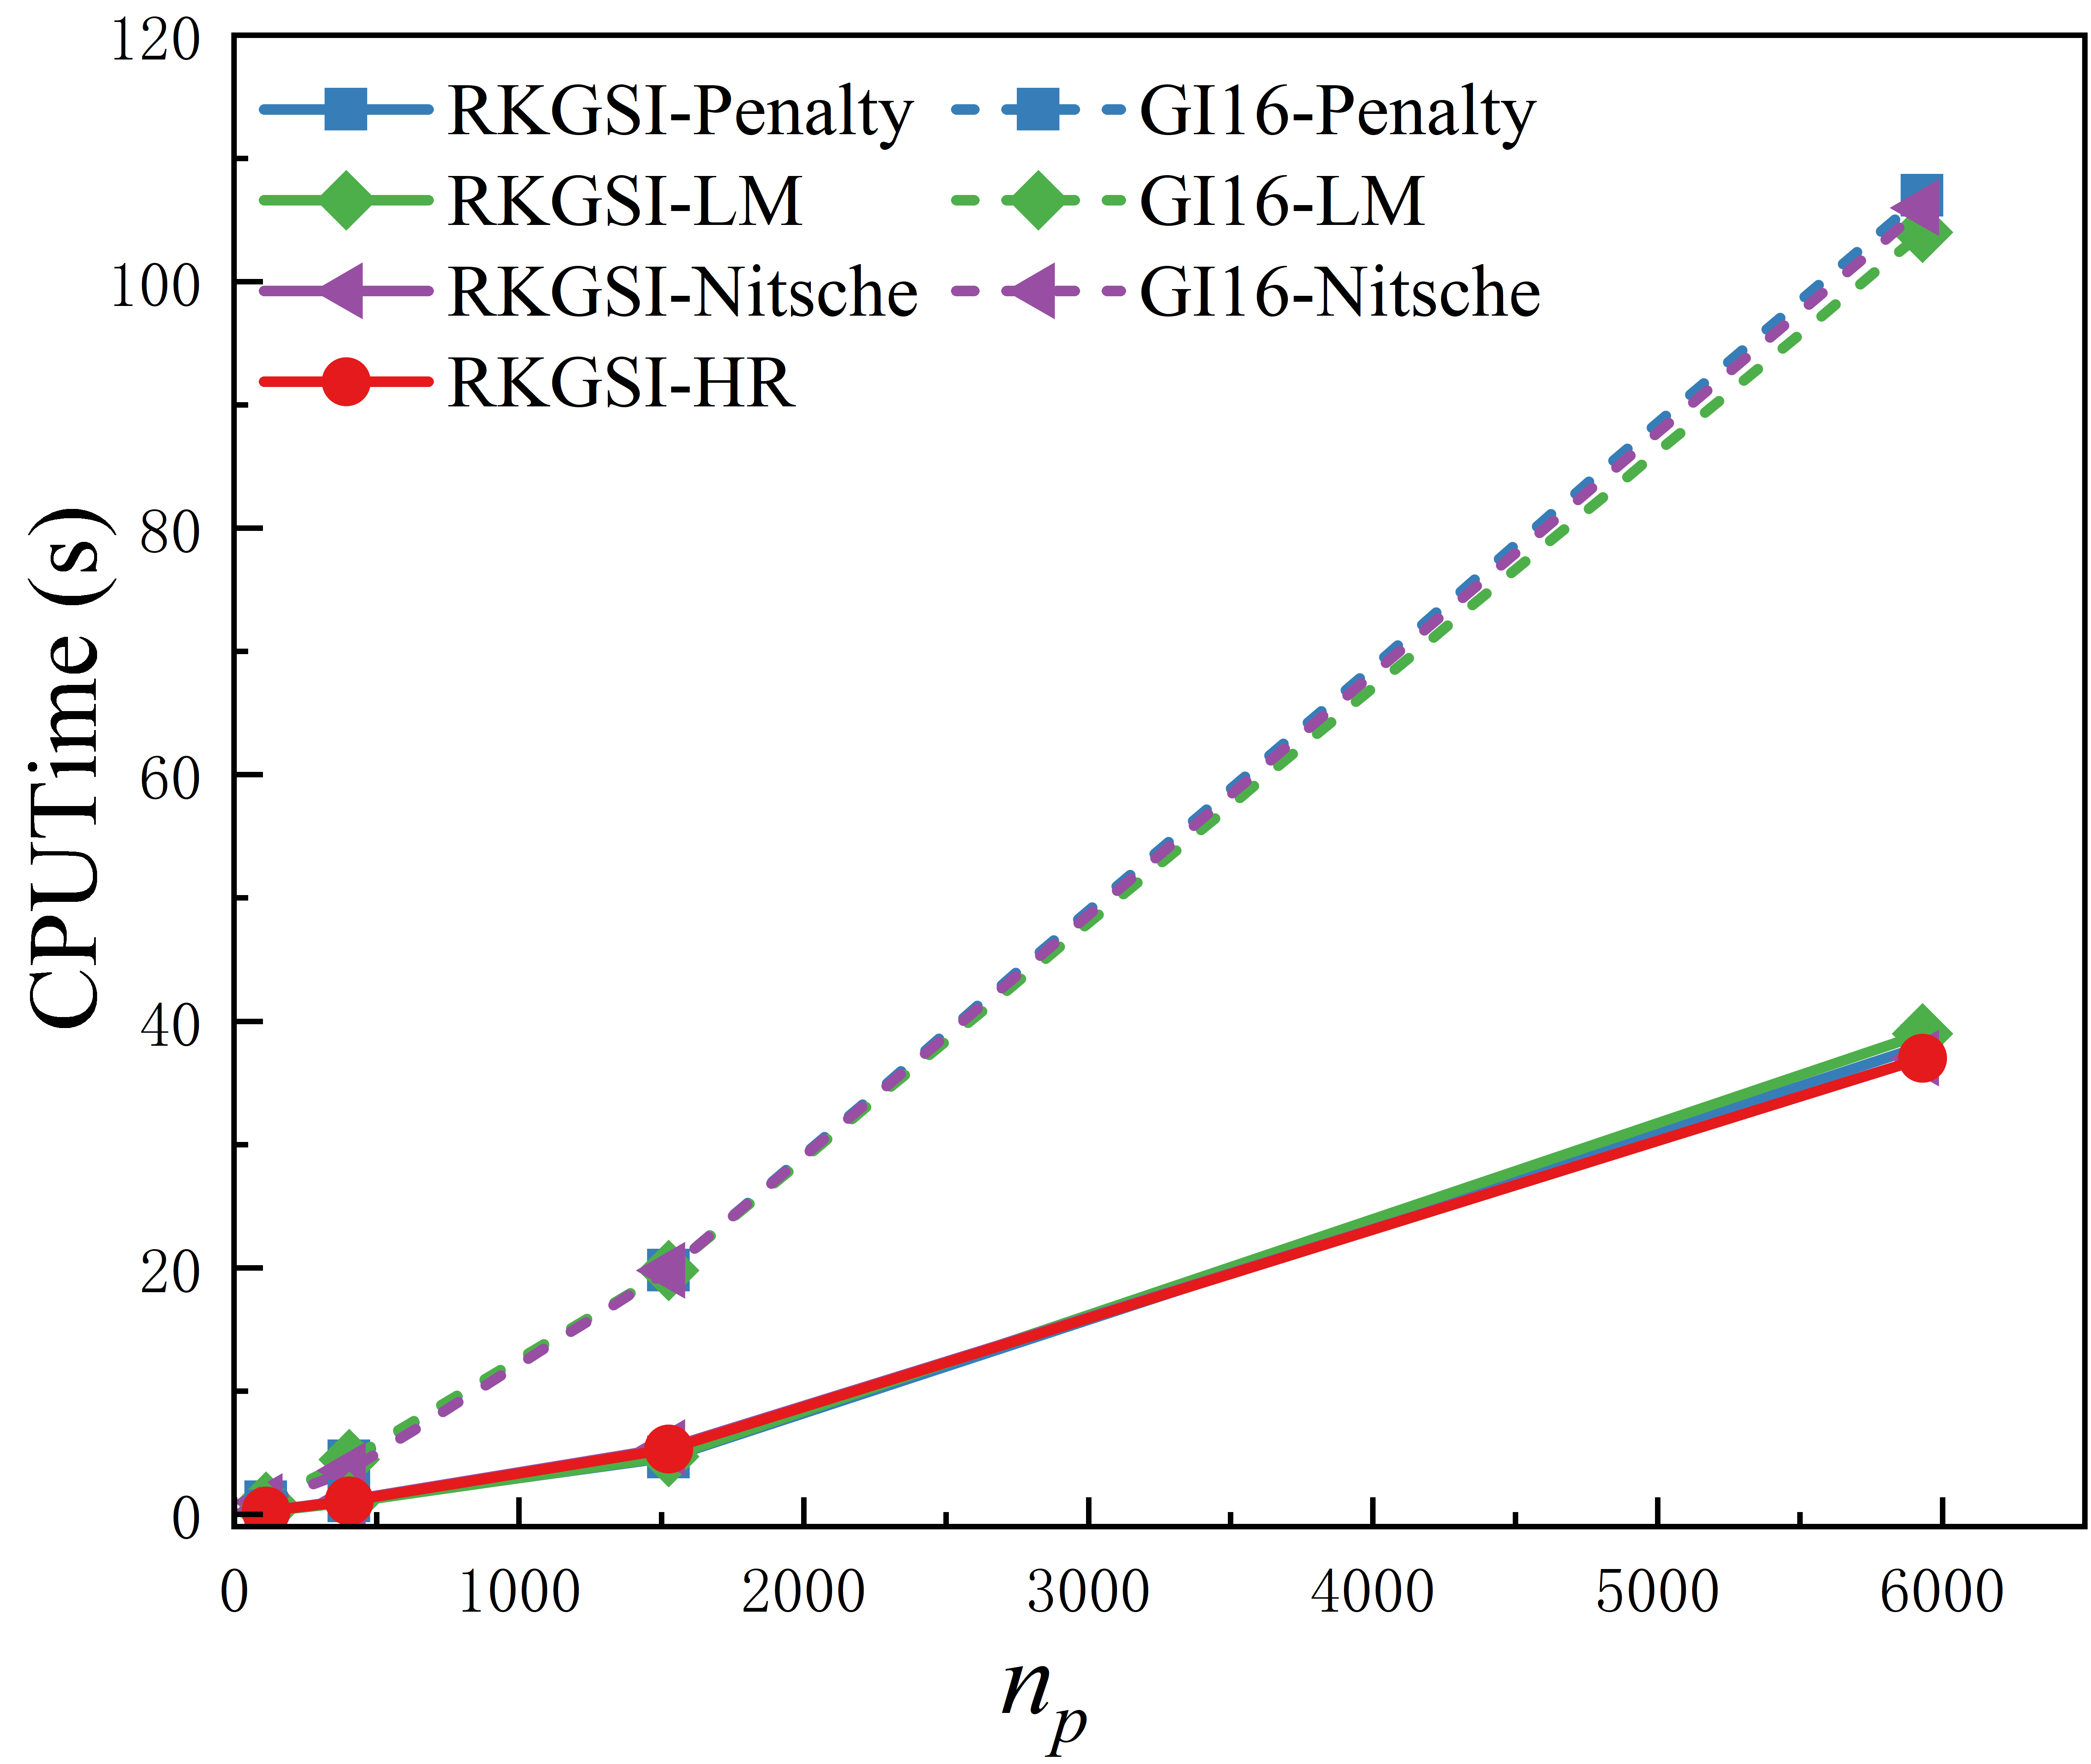
\includegraphics[width=0.49\textwidth]{figure/EHR/hole/cputime.png}
    \phantomcaption\label{Hcputime}
    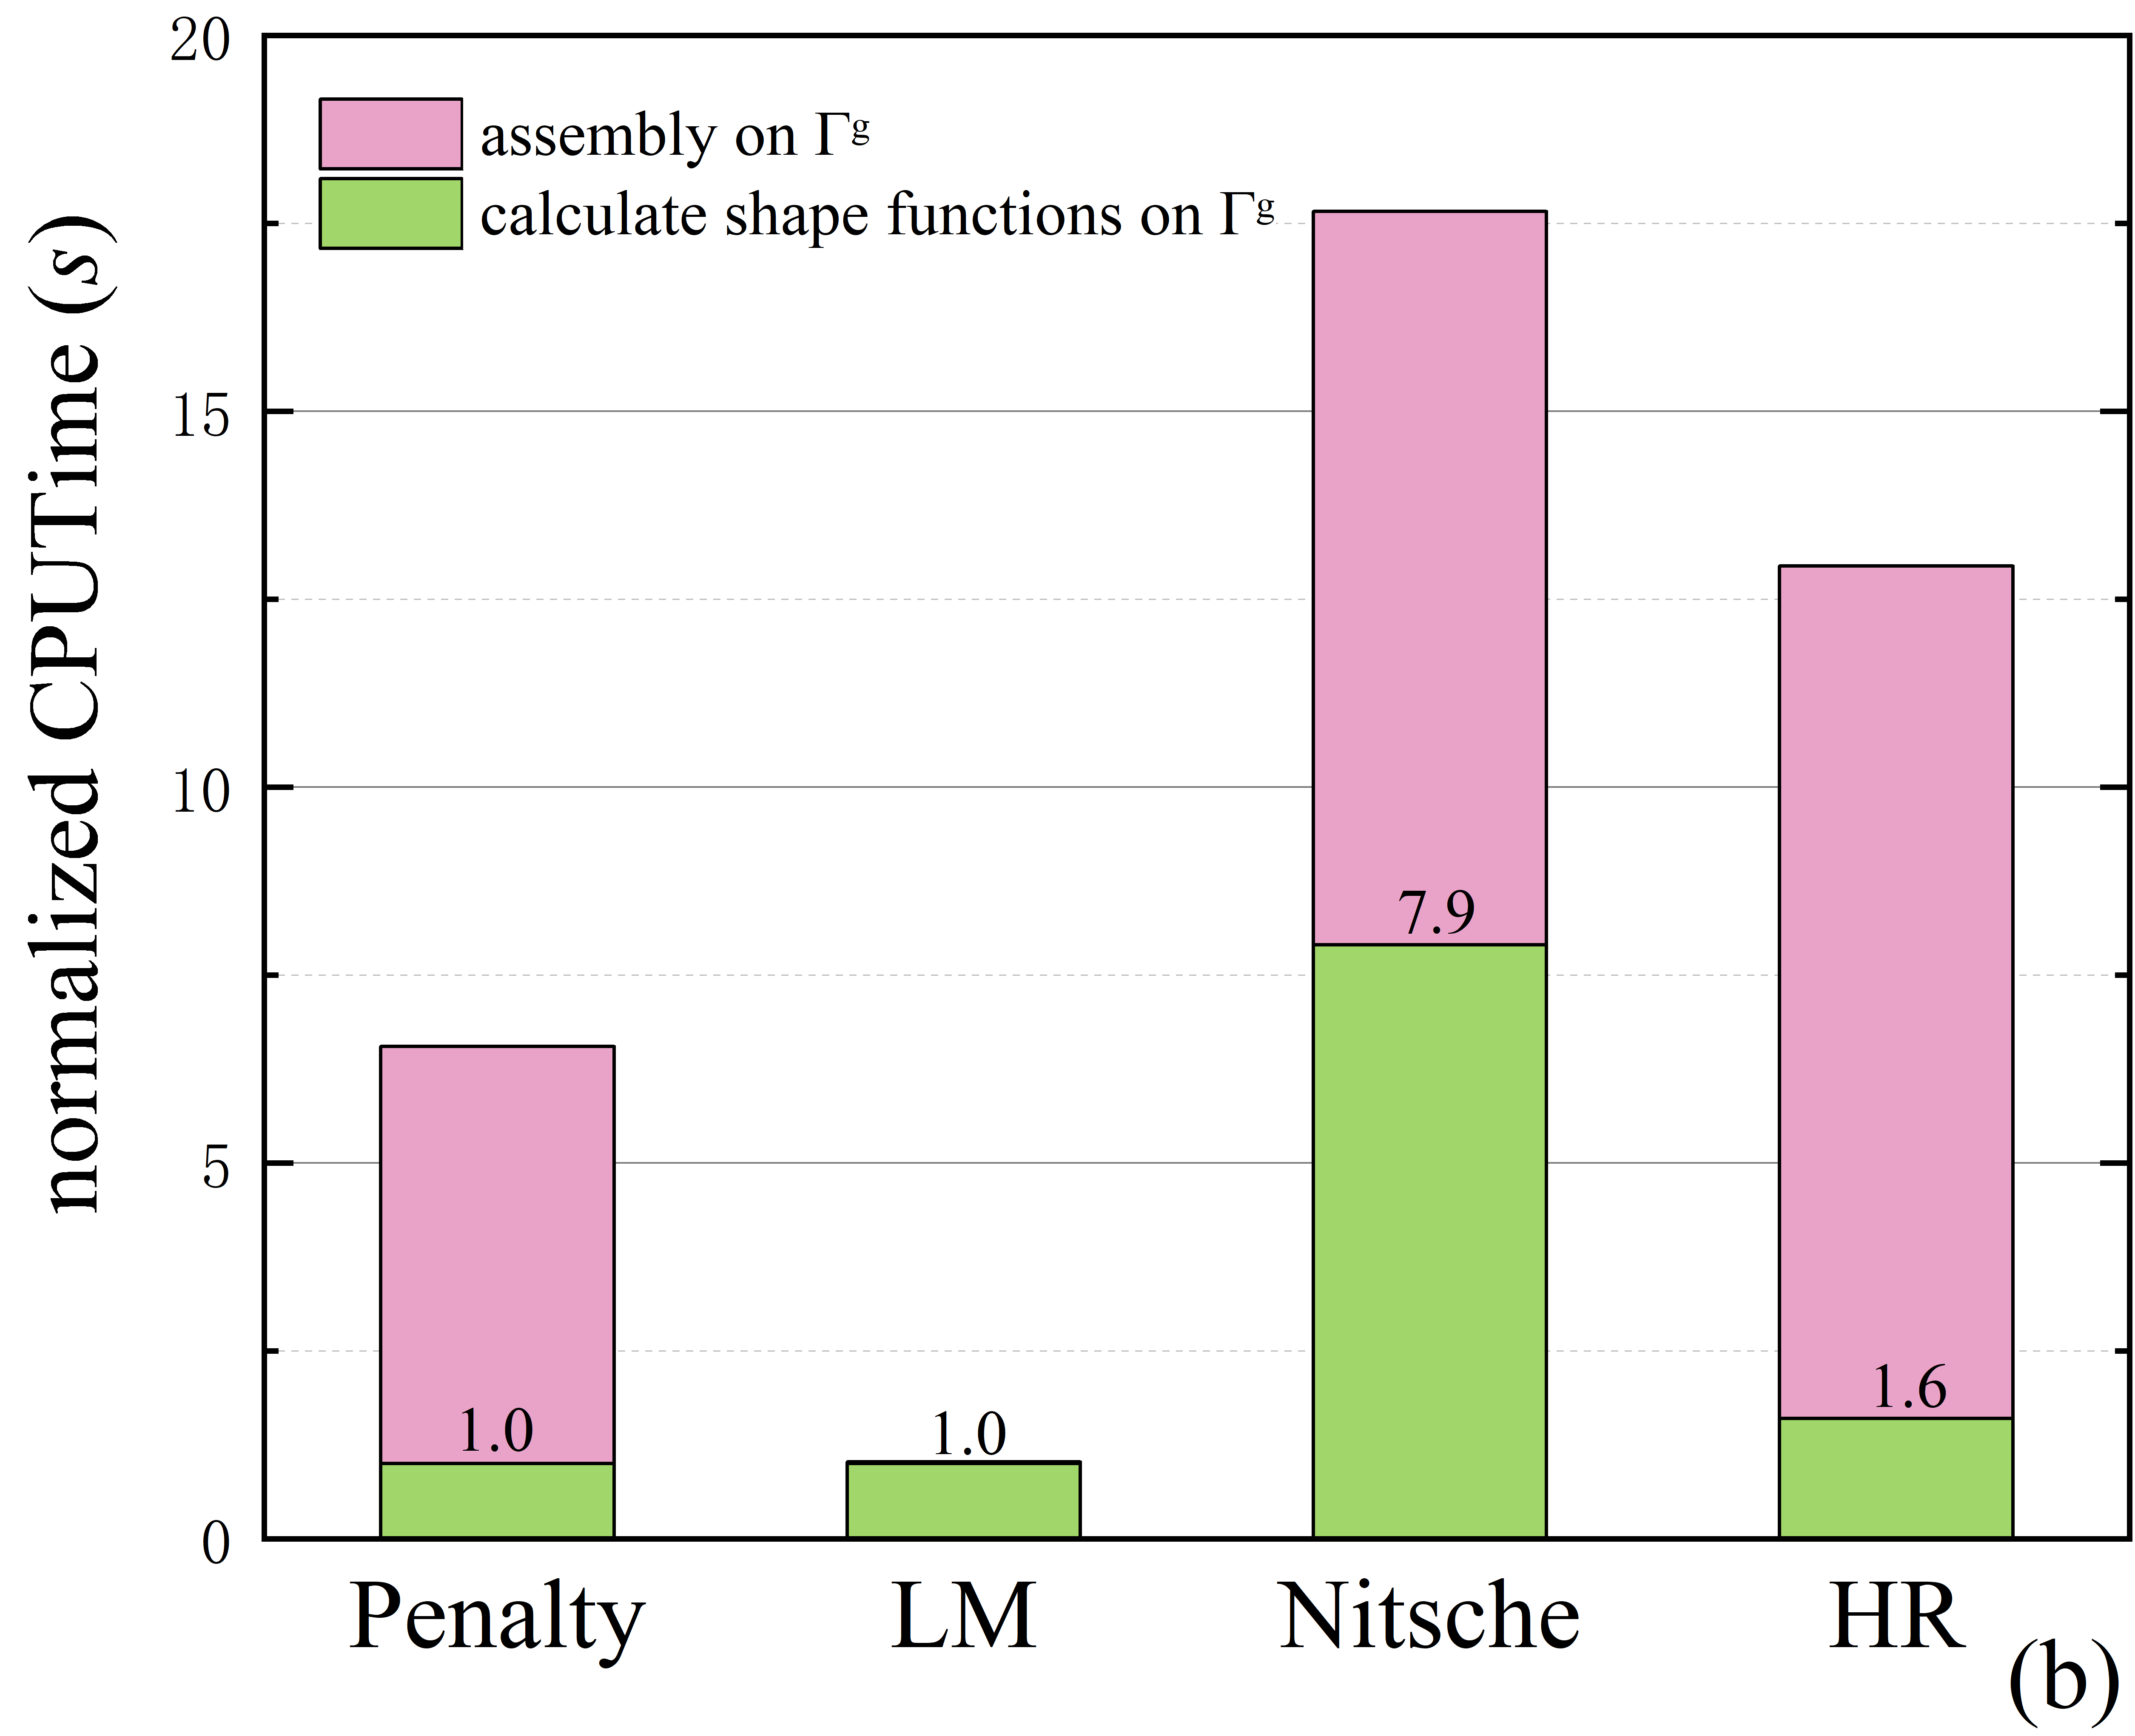
\includegraphics[width=0.49\textwidth]{figure/EHR/hole/efficiency.png}
    \phantomcaption\label{Hefficiency}
\end{subcaptiongroup}
\caption{\centering{带孔无限大平板问题效率对比:\\\subref{Hcputime} 计算时间与节点数的关系;\subref{Hefficiency} 边界条件施加效率分析}}
\end{figure} 
\section{小结}
本章介绍了一种基于赫林格-赖斯纳变分原理的变分一致性本质边界条件施加方法,用于求解弹性力学问题。该方法通过采用混合离散近似赫林格-赖斯纳变分原理弱形式中的位移和应力,实现了满足积分约束条件的一种本质边界条件施加方法。
具体来说,该方法在离散平衡方程中,采用传统无网格形函数对位移进行离散,而将应力在每个背景积分域上近似为对应阶次的多项式。在赫林格-赖斯纳变分原理的框架下,该方法的离散平衡方程具有类似传统Nitsche法的格式,可以视为再生光滑梯度积分法的一种新型Nitsche法。
相较于传统Nitsche法,该方法的修正变分项采用了无网格形函数和再生光滑梯度的混合离散,从而在确保变分一致性的同时避免了复杂且耗时的形函数导数计算,明显提高了计算效率。
与此同时该方法中的稳定项直接源于赫林格-赖斯纳变分原理的弱形式,无需额外增加稳定项,并且稳定项中不包含任何人工参数。
这有效消除了传统Nitsche法中人工参数依赖性的问题。
之后进一步通过典型算例的系统验证所提方法基于赫林格-赖斯纳变分原理施加本质边界条件的变分一致性、计算精度和计算效率。
结果表明,该方法在保持变分一致性的同时,能够提供较高的计算精度,并且相比传统Nitsche法也有效的提高了计算效率。
\begin{figure}[H]
    \centering
    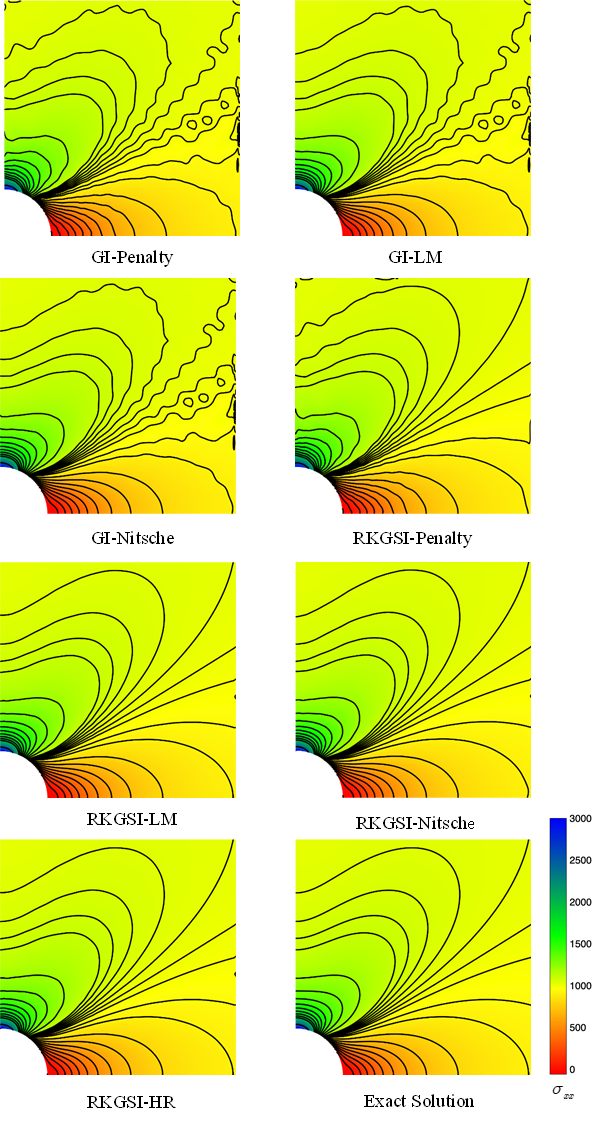
\includegraphics[scale=1.1]{figure/EHR/hole/sigmaxx.png}
\caption{带孔无限大平板问题$\sigma_{xx}$应力云图}\label{sigmaxx}
\end{figure}

\chapter{薄板问题HR}
本章进一步介绍了带有挠度和弯矩双变量时薄板问题Hellinger-Reissner变分原理,随后通过对挠度采用再生核近似离散,弯矩在每个背景积分单元建立局部多项式离散的方式
构造了一种基于Hellinger-Reissner变分原理的变分一致性本质边界条件施加方法,最后通过数值算例进一步验证在高阶薄板问题时所提方法的变分一致性、计算精度和计算效率。
\section{Hellinger-Reissner变分原理}
Hellinger-Reissner变分原理不仅适用于解决弹性力学问题中的位移和应力之间的耦合现象,并且在结构力学中也广泛应用于薄板和壳体等问题的数值求解,
Hellinger-Reissner变分原理基于能量泛函的最小化原理,在薄板问题中引入了两个变分函数:挠度场的变分函数和弯矩场的变分函数。
通过构造能量泛函和变分操作,得到平衡方程和边界条件的弱形式,并通过数值方法求解离散化的方程组获得薄板的挠度和弯矩分布。
\par
基于Hellinger-Ressiner变分原理\cite{},四阶薄板问题控制方程式(\ref{P control equation})对应的余能泛函表达式为:
\begin{equation}\label{pfanhan}
\begin{split}
    \Pi_{H\!R}(M_{\alpha\beta},w)&=\int_{\Omega}\frac{1}{2}M_{\alpha\beta}C^{-1}_{\alpha\beta\gamma\eta}M_{\gamma\eta}d\Omega-\int_{\Gamma_w}V_{\pmb n}\bar{w}d\Gamma+\int_{\Gamma_{\theta}}M_{\pmb{nn}}\bar{\theta}_nd\Gamma-p\bar{w}\vert_{x\in{c_w}}\\
&+\int_{\Omega}w(M_{\alpha\beta,\alpha\beta}+\bar{q})d\Omega+\int_{\Gamma_M}w_{,\pmb n}(M_{\pmb{nn}}-\bar{M}_{\pmb{nn}})d\Gamma\\
&-\int_{\Gamma_V}w(V_{\pmb n}-\bar{V}_{\pmb n})d\Gamma-w(P-\bar{P})\vert_{x\in{c_P}}
\end{split}
\end{equation}\par
对余能泛函$\Pi_{H\!R}$进行变分得到式(\ref{P control equation})中带有挠度$w$和弯矩$M$双变量的伽辽金弱形式:
\newpage
\begin{equation}\label{Pweakfrom}
\begin{split}
    \delta\Pi_{H\!R}(M_{\alpha\beta,w})&=\int_{\Omega}\delta M_{\alpha\beta}D^{-1}_{\alpha\beta\gamma\eta}M_{\gamma\eta}d\Omega-\int_{\Gamma_w}\delta V_{\pmb n}\bar{w}d\Gamma+\int_{\Gamma_{\theta}}\delta M_{\pmb{nn}}\bar{\theta}_nd\Gamma-\delta P\bar{w}_{x\in{c_w}}\\
    &+\int_{\Omega}\delta M_{\alpha\beta,\alpha\beta}wd\Omega+\int_{\Gamma_M}\delta M_{\pmb{nn}}w_{,\pmb n}d\Gamma-\int_{\Gamma_V}\delta V_{\pmb n}wd\Gamma-\delta Pw\vert_{x\in{c_P}}\\
    &+\int_{\Omega}\delta w(M_{\alpha\beta,\alpha\beta}+\bar{q})d\Omega+\int_{\Gamma_M}\delta w_{,n}(M_{nn}-\bar{M}_{nn})d\Gamma\\
    &-\int_{\Gamma_V}\delta w(V_{\pmb n}-\bar{V}_{\pmb n})d\Gamma-\delta w(P-\bar{P})\vert_{x\in{c_P}}\\
    &=0
\end{split}
\end{equation}\par
对能量泛函$\Pi_{H\!R}$取极值时,要求对任意的$\delta w$、$\delta M_{\alpha\beta}$关于$\delta\Pi_{H\!R}$都要恒成立,此时利用几何关系式:
\begin{equation}
    \begin{split}
    \Gamma=\Gamma_w\cup\Gamma_V\cup\Gamma_{\theta}\cup\Gamma_M,c=c_w\cup c_P\\
    \Gamma_w\cap\Gamma_V=\Gamma_{\theta}\cap\Gamma_M=c_w\cap c_P=\varnothing
\end{split}
\end{equation}
进一步将弱形式(\ref{Pweakfrom})根据$\delta w$、$\delta M_{\alpha\beta}$改写为下列两式:
\begin{equation}\label{Pweakform1}
    \begin{split}
        \int_\Omega {\delta {M_{\alpha \beta }}D_{\alpha \beta \gamma \eta }^{ - 1}{M_{\gamma \eta }}d\Omega }&=\int_\Gamma  {\delta {V_{\bf{n}}}wd\Gamma }  - \int_\Gamma  {\delta {M_{{\bf{nn}}}}{w_{,{\bf{n}}}}d\Gamma }+{\left. {\delta Pw} \right|_{{\bf{x}} \in c}} - \int_\Omega  {\delta {M_{\alpha \beta ,\alpha \beta }}wd\Omega } \\
        &-\int_{{\Gamma _w}} {\delta {V_{\bf{n}}}wd\Gamma }  + \int_{{\Gamma _\theta }} {\delta {M_{{\bf{nn}}}}{w_{,{\bf{n}}}}d\Gamma }  - {\left. {\delta Pw} \right|_{{\bf{x}} \in {c_w}}}\\
        &+\int_{{\Gamma _w}} {\delta {V_{\bf{n}}}\bar wd\Gamma }  - \int_{{\Gamma _\theta }} {\delta {M_{{\bf{nn}}}}{{\bar \theta }_{\bf{n}}}d\Gamma }  + {\left. {\delta P\bar w} \right|_{{\bf{x}} \in {c_w}}}
    \end{split}
\end{equation}
\begin{equation}
        \begin{split}\label{Pweakform2}
            &\int_\Gamma  {\delta w{V_{\bf{n}}}d\Gamma } - \int_\Gamma  {\delta {w_{,{\bf{n}}}}{M_{{\bf{nn}}}}d\Gamma }  + {\left. {\delta wP} \right|_{{\bf{x}} \in c}} - \int_\Omega  {\delta w{M_{\alpha \beta ,\alpha\beta}}d\Omega }\\
            &- \int_{{\Gamma _w}} {\delta w{V_{\bf{n}}}d\Gamma }  + \int_{{\Gamma _\theta }} {\delta {w_{,{\bf{n}}}}{M_{{\bf{nn}}}}d\Gamma }  - {\left. {\delta wP} \right|_{{\bf{x}} \in {c_w}}}\\
            &= \int_{{\Gamma _V}} {\delta w{{\bar V}_{\bf{n}}}d\Gamma }  - \int_{{\Gamma _M}} {\delta {w_{,{\bf{n}}}}{{\bar M}_{{\bf{nn}}}}d\Gamma }  + {\left. {\delta w\bar P} \right|_{{\bf{x}} \in {c_P}}} + \int_\Omega  {\delta w\bar qd\Omega} 
    \end{split}
\end{equation} 
\section{挠度-弯矩混合离散}
薄板挠度$w$采用基于再生核近似的无网格形函数进行离散。无网格法通过在薄板中面$\Omega$和边界$\Gamma$上布置一系列无网格节点$\{\pmb{x}_I\}^{N\!P}_{I=1}$进行离散,
不失为一般性,考虑任意薄板挠度$w$的近似表达式$w^h$及其虚位移$\delta w^h$可表示为:
\begin{equation}\label{w}
\begin{split}
    w^h(\pmb{x})=\sum_{I=1}^{N\!P}\Psi_I(\pmb{x})d_{I},\delta w^h(\pmb{x})=\sum_{I=1}^{N\!P}\Psi_I(\pmb{x})\delta d_I
\end{split}
\end{equation}
其中$N\!P$表示无网格节点数量,$d_I$、$\Psi_I(\pmb{x})$为无网格节点$\pmb{x}_I$上的节点系数和无网格形函数。
根据再生核近似理论\cite{}以及满足多项式一致性条件,无网格形函数的表达式为:
\begin{equation}
\begin{split}
    \Psi_I(\pmb{x})=\pmb{p}^T(\pmb{0})\pmb{A}^{-1}(\pmb{x})\pmb{p}(\pmb{x}_I-\pmb{x})\phi_s(\pmb{x}_I-\pmb{x})
\end{split}
\end{equation}
其中$\pmb{p}$为$p$阶的多项式基函数向量,$\pmb{A}$为矩量矩阵,核函数$\phi_s(\pmb{x}_I-\pmb{x})$选取五次样条函数。具体求解过程见第一章。\par
% \begin{figure}[H]
%     \centering
%     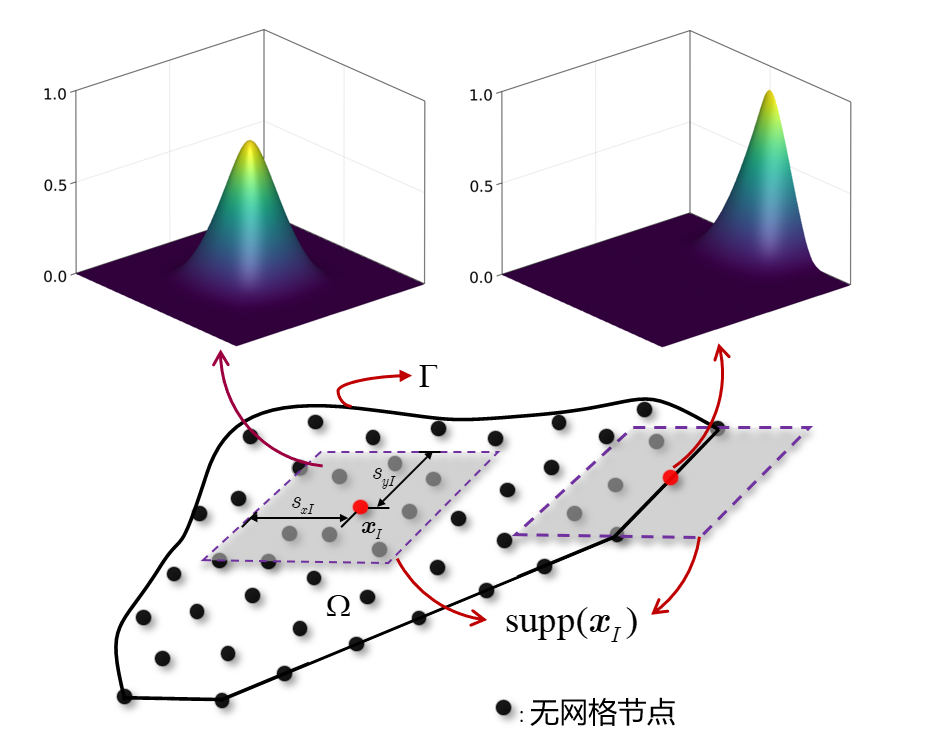
\includegraphics[scale=0.6]{figure/PHR/PSI.png}
%     \caption{薄板无网格离散}\label{PPSI}
% \end{figure}
弯矩分量$M_{\alpha\beta}$在每个背景积分单元建立局部的多项式进行离散。
如图(\ref{Pintegralscheme})所示,将薄板中面$\Omega$划分为一系列背景积分单元$\Omega_C,C=1,2,\dotsb,n_C$,并且存在$\cup_{C=1}^{N\!C}\Omega_C\thickapprox\Omega$。
在背景积分单元$\Omega_C$内,假定弯矩分量$M_{\alpha\beta}$以任意的多项式进行离散,并将离散后的弯矩分量$M_{\alpha\beta}$记为$M_{\alpha\beta}^h$
\begin{equation}\label{moment}
\begin{split}
    M^h_{\alpha\beta}(\pmb{x})=\pmb{a}_{\alpha\beta}^T\tilde{\pmb{q}}(\pmb{x})
\end{split}
\end{equation}
$\tilde{\pmb{q}}(\pmb{x})$是比多阶基函数向量$\pmb{p}(\pmb{x})$低两阶的单项式向量,具体表达式为:
\begin{equation}
\begin{split}
    \tilde{\pmb{q}}(\pmb{x})=\{1,\;x,\;y,\;\dots,\;x^iy^j,\;\dots,\;y^{p-2}\}^T,0 \le i+j \le p-2
\end{split}
\end{equation}\par
$\pmb{a}_{\alpha\beta}$为弯矩分量$M_{\alpha\beta}$在积分域$\Omega_C$内的常系数向量,此时将离散的弯矩分量表达式(\ref{moment})代入式(\ref{Pweakform1})同时根据式(\ref{MVP})和线弹性本构关系式(\ref{Malphabeta})可以得到:
\begin{equation}
\begin{split}
    \int_{\Omega}\delta\pmb{a}_{\alpha\beta}^T\tilde{\pmb{q}}D^{-1}_{\alpha\beta\gamma\eta}\pmb{a}_{\gamma\eta}^T\tilde{\pmb{q}}d\Omega&=
    -\int_{\Gamma}D_{\alpha\beta\gamma\eta}^{-1}\mathcal{V}_{\alpha\beta}\delta\pmb{a}_{,\alpha\beta}^T\tilde{\pmb{q}}wd\Gamma
    +\int_{\Gamma}D_{\alpha\beta\gamma\eta}^{-1}\mathcal{M}_{\alpha\beta}\delta\pmb{a}_{,\alpha\beta}^T\tilde{\pmb{q}}w_{,\pmb{n}}d\Gamma\\
    &-D_{\alpha\beta\gamma\eta}^{-1}\mathcal{P}_{\alpha\beta}\delta\pmb{a}_{,\alpha\beta}^T\tilde{\pmb{q}}w\vert_{x\in c}
    -\int_{\Omega}\delta\pmb{a}_{\alpha\beta,\alpha\beta}^T\tilde{\pmb{q}}wd\Omega\\
    &+\int_{\Gamma_w}D_{\alpha\beta\gamma\eta}^{-1}\mathcal{V}_{\alpha\beta}\delta\pmb{a}_{,\alpha\beta}^T\tilde{\pmb{q}}d\Gamma
    -\int_{\Gamma_{\theta}}D_{\alpha\beta\gamma\eta}^{-1}\mathcal{M}_{\alpha\beta}\delta\pmb{a}_{,\alpha\beta}^T\tilde{\pmb{q}}w_{,\pmb{n}}d\Gamma\\
    &+D_{\alpha\beta\gamma\eta}^{-1}\mathcal{P}_{\alpha\beta}\delta\pmb{a}_{,\alpha\beta}^T\tilde{\pmb{q}}wx\vert_{x\in{c_w}}
    -\int_{\Gamma_w}D_{\alpha\beta\gamma\eta}^{-1}\mathcal{V}_{\alpha\beta}\delta\pmb{a}_{,\alpha\beta}^T\tilde{\pmb{q}}\bar{w}d\Gamma\\
    &+\int_{\Gamma_{\theta}}D_{\alpha\beta\gamma\eta}^{-1}\mathcal{M}_{\alpha\beta}\delta\pmb{a}_{,\alpha\beta}^T\tilde{\pmb{q}}\bar{\theta}_{\pmb{n}}d\Gamma
    -D_{\alpha\beta\gamma\eta}^{-1}\mathcal{P}_{\alpha\beta}\delta\pmb{a}_{,\alpha\beta}^T\tilde{\pmb{q}}\bar{w}\vert_{x\in{c_w}}
\end{split}
\end{equation}
进一步将等式两边同时消去$\delta\pmb{a}^T_{\alpha\beta}$:
\begin{equation}
\begin{split}
        \int_{\Omega}\tilde{\pmb{q}}D^{-1}_{\alpha\beta\gamma\eta}\pmb{a}_{\gamma\eta}^T\tilde{\pmb{q}}d\Omega&=
        -\int_{\Gamma}D_{\alpha\beta\gamma\eta}^{-1}\mathcal{V}_{\alpha\beta}\tilde{\pmb{q}}wd\Gamma
        +\int_{\Gamma}D_{\alpha\beta\gamma\eta}^{-1}\mathcal{M}_{\alpha\beta}\tilde{\pmb{q}}w_{,\pmb{n}}d\Gamma\\
        &-D_{\alpha\beta\gamma\eta}^{-1}\mathcal{P}_{\alpha\beta}\tilde{\pmb{q}}w\vert_{x\in c}
        -\int_{\Omega}\delta\tilde{\pmb{a}}_{\alpha\beta,\alpha\beta}^T\tilde{\pmb{q}}wd\Omega\\
        &+\int_{\Gamma_w}D_{\alpha\beta\gamma\eta}^{-1}\mathcal{V}_{\alpha\beta}\tilde{\pmb{q}}d\Gamma
        -\int_{\Gamma_{\theta}}D_{\alpha\beta\gamma\eta}^{-1}\mathcal{M}_{\alpha\beta}\tilde{\pmb{q}}w_{,\pmb{n}}d\Gamma\\
        &+D_{\alpha\beta\gamma\eta}^{-1}\mathcal{P}_{\alpha\beta}\tilde{\pmb{q}}wx\vert_{x\in{c_w}}
        -\int_{\Gamma_w}D_{\alpha\beta\gamma\eta}^{-1}\mathcal{V}_{\alpha\beta}\tilde{\pmb{q}}\bar{w}d\Gamma\\
        &+\int_{\Gamma_{\theta}}D_{\alpha\beta\gamma\eta}^{-1}\mathcal{M}_{\alpha\beta}\tilde{\pmb{q}}\bar{\theta}_{\pmb{n}}d\Gamma
        -D_{\alpha\beta\gamma\eta}^{-1}\mathcal{P}_{\alpha\beta}\tilde{\pmb{q}}\bar{w}\vert_{x\in{c_w}}
\end{split}
\end{equation}
对上式进行移项得到常系数向量$\pmb{a}_{\alpha\beta}$的具体表达式:
\begin{equation}\label{aalphabeta}
\begin{split}
    \pmb{a}_{\gamma\eta}=-D_{\alpha\beta\gamma\eta}\tilde{\pmb{G}}^{-1}(\sum_{I=1}^{N\!P}(\tilde{g}_{\alpha\beta I}-\bar{g}_{\alpha\beta I})d_I+\hat{g}_{\alpha\beta})
\end{split}
\end{equation}
其中:
\begin{align}
\label{PG}&\tilde{\pmb{G}}=\int_{\Omega_C}\tilde{\pmb{q}}\tilde{\pmb{q}}^Td\Omega\\
\label{Pg1}&\tilde{g}_{\alpha\beta I}=\int_{\Gamma_C}\Psi_{I,n}\tilde{\pmb{q}}n_{\alpha}n_{\beta}d\Gamma-\int_{\Gamma_C}\Psi_I(n_{\alpha}\tilde{\pmb{q}}_{,\beta}+\tilde{\pmb q}_{,\gamma}s_{\alpha}n_{\beta}s_{\gamma})d\Gamma
+[[\Psi_I\tilde{\pmb q}n_{\alpha}s_{\beta}]]\vert_{x\in c_C}+\int_{\Omega_C}\Psi_I\tilde{\pmb{q}}_{,\alpha\beta}d\Omega\\
\label{Pg2}&\bar{g}_{\alpha\beta I}=\int_{{\Gamma_{\theta}}\cap{\Gamma_C}}\Psi_{I,n}\tilde{\pmb{q}}n_{\alpha}n_{\beta}d\Gamma-\int_{{\Gamma_w}\cap{\Gamma_C}}\Psi_I(n_{\alpha}\tilde{\pmb{q}}_{,\beta}+\tilde{\pmb q}_{,\gamma}s_{\alpha}n_{\beta}s_{\gamma})d\Gamma
+[[\Psi_I\tilde{\pmb q}n_{\alpha}s_{\beta}]]\vert_{x\in{c_w}\cap{c_C}}\\
\label{Pg3}&\hat{g}_{\alpha\beta I}=\int_{{\Gamma_{\theta}}\cap{\Gamma_C}}\tilde{\pmb{q}}n_{\alpha}n_{\beta}\bar{\theta}_nd\Gamma-\int_{{\Gamma_w}\cap{\Gamma_C}}(n_{\alpha}\tilde{\pmb{q}}_{,\beta}+\tilde{\pmb q}_{,\gamma}s_{\alpha}n_{\beta}s_{\gamma})\bar{w}d\Gamma
+[[\bar{w}\tilde{\pmb q}n_{\alpha}s_{\beta}]]\vert_{x\in{c_w}\cap{c_C}}
\end{align}
式中$\Gamma_C$是$\Omega_C$的边界,此时将$\pmb{a}_{\alpha\beta}$代入到式(\ref{moment})中得到近似的弯矩分量$M^h_{\alpha\beta}(\pmb{x})$的表达式:
\begin{equation}
\begin{split}
M^h_{\alpha\beta}(\pmb{x})&=\tilde{\pmb{q}}^T(\pmb{x})\pmb a_{\alpha\beta}\\
&=-D_{\alpha\beta\gamma\eta}(\sum_{I=1}^{N\!P}(\tilde{\pmb q}^T(\pmb x)\tilde{\pmb G}^{-1}\tilde{g}_{\gamma\eta I}-\tilde{\pmb q}^T(\pmb x)\tilde{\pmb G}^{-1}\bar{g}_{\gamma\eta I})d_I+\tilde{\pmb q}^T(\pmb x)\tilde{\pmb G}^{-1}\hat{g}_{\gamma\eta})\\
&=-D_{\alpha\beta\gamma\eta}(\sum_{I=1}^{N\!P}\tilde{\Psi}_{I,\gamma\eta}(\pmb x)d_I-\sum_{I=1}^{N\!P}\bar{\Psi}_{I,\gamma\eta}(\pmb{x})d_I+\tilde{\pmb q}^T(\pmb x)\tilde{\pmb G}^{-1}\hat{g}_{\gamma\eta})
\end{split}
\end{equation}
其中:
\begin{align}
 \label{PTPSI}&\tilde{\Psi}_{I,\alpha\beta}=\tilde{\pmb q}^T(\pmb x)\tilde{\pmb G}^{-1}\tilde{g}_{\alpha\beta I}\\
 \label{PBPSI}&\bar{\Psi}_{i,\alpha\beta}=\tilde{\pmb q}^T(\pmb x)\tilde{\pmb G}^{-1}\bar{g}_{\alpha\beta I}\quad \pmb{x}\in\Omega_C
\end{align}\par
此时,弯矩分量表达式中的$\tilde{\Psi}_{I,\alpha\beta}$是根据再生光滑梯度理论\cite{}构造的二阶再生光滑梯度,可以避免传统无网格形函数梯度的复杂计算从而提高梯度计算效率,而$\tilde{\mathfrak{g}}_{\alpha\beta I}$是满足Galerkin变分一致性的积分约束条件,进而保证算法的计算精度和误差收敛性。
同时$\bar{\Psi}_{I,\alpha\beta}$为在本质边界条件上求值的新型光滑梯度表达式。
% \begin{figure}[H]
%     \centering
%     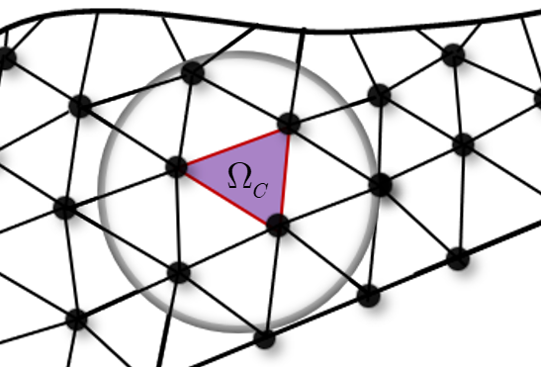
\includegraphics[scale=0.6]{figure/PHR/momentlisan.png}
%     \caption{背景积分单元示意图}\label{momentlisan}
% \end{figure}
\section{Hellinger-Reissner变分原理下的本质边界条件施加方法}
通过式(\ref{Pweakfrom})看出在四阶薄板问题上基于Hellinger-Reissner变分原理得到的弱形式中已经考虑了本质边界条件和自然边界条件。
为了更好的研究Hellinger-Reissner变分原理在求解薄板问题上的本质边界条件施加方法,此时将挠度离散表达式(\ref{w})和弯矩离散表达式(\ref{moment})代入到式(\ref{Pweakform2})中得到:
{\setlength\abovedisplayskip{0.5cm}
\setlength\belowdisplayskip{0.5cm}
\begin{equation}
\begin{split}
    &\int_{\Gamma}\sum_{I=1}^{N\!P}\Psi_I\delta{d_I}\mathcal{V}_{\alpha\beta}w_{,\alpha\beta}d\Gamma-\int_{\Gamma}\sum_{I=1}^{N\!P}\Psi_{I,n}\delta{d_I}\mathcal{M}_{\alpha\beta}w_{,\alpha\beta}d\Gamma+\sum_{I=1}^{N\!P}\Psi_I\delta{d_I}\mathcal{P}_{\alpha\beta}w_{,\alpha\beta}\vert_{x\in c}\\
    &-\int_{\Omega}\sum_{I=1}^{N\!P}\Psi_I\delta{d_I}\pmb{a}^T_{\alpha\beta,\alpha\beta}\tilde{\pmb q}d\Omega-\int_{\Gamma_w}\sum_{I=1}^{N\!P}\Psi_I\delta{d_I}\mathcal{V}_{\alpha\beta}w_{,\alpha\beta}d\Gamma\\
    &+\int_{\Gamma_{\theta}}\sum_{I=1}^{N\!P}\Psi_{I,n}\delta{d_I}\mathcal{M}_{\alpha\beta}w_{,\alpha\beta}d\Gamma
    -\sum_{I=1}^{N\!P}\Psi_I\delta{d_I}\mathcal{P}_{\alpha\beta}w_{,\alpha\beta}\vert_{x\in c_w}\\
    &=\sum_{I=1}^{N\!P}\int_{\Gamma_V}\Psi_I\delta{d_I}\bar{V}_{\pmb n}d\Gamma-\sum_{I=1}^{N\!P}\int_{\Gamma_M}\Psi_{I,n}\delta{d_I}\bar{M}_{\pmb{nn}}d\Gamma\\
    &+\sum_{I=1}^{N\!P}\Psi_I\delta{d_I}\bar{P}\vert_{x\in{c_P}}+\sum_{I=1}^{N\!P}\int_{\Omega}\Psi_I\delta{d_I}\bar{q}d\Omega
\end{split}
\end{equation}}
此时引入式(\ref{MVP1})并根据薄板问题线弹性本构关系式(\ref{Malphabeta})得出:
\begin{equation}\label{2}
\begin{split}
  -\sum_{C=1}^{N\!C}(\tilde{g}_{\alpha\beta I}^T-\tilde{g}_{\alpha\beta I}^T)\pmb a_{\alpha\beta}=\pmb{f}
\end{split}
\end{equation}
其中$\pmb{f}$为外力向量,具体表达式为:
\begin{equation}
\begin{split}
    \pmb{f}=\int_{\Gamma_V}\Psi_I\bar{V}_{\pmb n}d\Gamma-\int_{\Gamma_M}\Psi_{I,n}\bar{M}_{\pmb{nn}}d\Gamma+\Psi_I\bar{P}\vert_{x\in{c_P}}+\int_{\Omega}\Psi_I\bar{q}d\Omega
\end{split}
\end{equation}
此时,进一步将式(\ref{aalphabeta})中的$\pmb{a}_{\alpha\beta}$代入到式(\ref{2})中可以得到:
\begin{equation}
\begin{split}\label{Pzuzhuang}
    &-\sum_{C=1}^{N\!C}(\tilde{g}_{\alpha\beta I}^T-\bar{g}_{\alpha\beta I}^T)a_{\alpha\beta}\\
    &=\sum_{C=1}^{N\!C}(\tilde{g}_{\alpha\beta I}^T-\bar{g}_{\alpha\beta I}^T)D_{\alpha\beta\gamma\eta}\tilde{\pmb{G}}^{-1}(\sum_{J=1}^{N\!P}(\tilde{g}_{\gamma\eta J}-\bar{g}_{\gamma\eta J})d_I+\hat{g}_{\gamma\eta})\\
    &=\sum_{C=1}^{N\!C}\sum_{J=1}^{N\!P}D_{\alpha\beta\gamma\eta}\tilde{g}_{\alpha\beta I}^T\tilde{\pmb G}^{-1}\tilde{g}_{\gamma\eta J}d_J\\
    &+\sum_{C=1}^{N\!C}\sum_{J=1}^{N\!P}D_{\alpha\beta\gamma\eta}(-\bar{g}_{\alpha\beta I}^T\tilde{\pmb G}^{-1}\tilde{g}_{\gamma\eta J}-\tilde{g}_{\alpha\beta I}^T\tilde{\pmb G}^{-1}\tilde{g}_{\gamma\eta J})d_J\\
    &-(-\sum_{C=1}^{N\!C}D_{\alpha\beta\gamma\eta}\tilde{g}_{\alpha\beta I}^T\tilde{\pmb G}^{-1}\hat{g}_{\gamma\eta })\\
    &+\sum_{C=1}^{N\!C}\sum_{J=1}^{N\!P}D_{\alpha\beta\gamma\eta}\bar{g}_{\alpha\beta I}^T\tilde{\pmb G}^{-1}\tilde{g}_{\gamma\eta J}d_J\\
    &-\sum_{C=1}^{N\!C}D_{\alpha\beta\gamma\eta}\bar{g}_{\alpha\beta I}^T\tilde{\pmb G}^{-1}\hat{g}_{\gamma\eta }
\end{split}
\end{equation}
通过引入式(\ref{PG})、(\ref{PTPSI})对式(\ref{Pzuzhuang})中的第一项进行推导可以得到:
\begin{equation}
\begin{split}
    &\sum_{C=1}^{N\!C}D_{\alpha\beta\gamma\eta}\tilde{g}_{\alpha\beta I}^T\tilde{\pmb G}^{-1}\tilde{g}_{\gamma\eta J}\\
    &=\sum_{C=1}^{N\!C}D_{\alpha\beta\gamma\eta}\tilde{g}_{\alpha\beta I}^T\tilde{\pmb G}^{-1}\int_{\Omega_C}\tilde{\pmb q}\tilde{\pmb q}^Td\Omega\tilde{\pmb G}^{-1}\tilde{g}_{\gamma\eta J}\\
    &=\sum_{C=1}^{N\!C}D_{\alpha\beta\gamma\eta}\int_{\Omega_C}\tilde{g}_{\alpha\beta I}^T\tilde{\pmb G}^{-1}\tilde{\pmb q}\tilde{\pmb q}^T\tilde{\pmb G}^{-1}\tilde{g}_{\gamma\eta J}d\Omega \\
    &=\int_{\Omega}\tilde{\Psi}_{I,\alpha\beta}D_{\alpha\beta\gamma\eta}\tilde{\Psi}_{J,\gamma\eta}d\Omega \\
    &=\pmb{K}
\end{split}
\end{equation}
\newpage
通过引入式(\ref{PTPSI})、(\ref{MVP1})对式(\ref{Pzuzhuang})中的第二项进行推导可以得到:
\begin{equation}
\begin{split}
    &-\sum_{C=1}^{N\!C}D_{\alpha\beta\gamma\eta}(\bar{g}_{\alpha\beta I}^T\tilde{\pmb G}^{-1}\tilde{g}_{\gamma\eta J}+\tilde{g}_{\alpha\beta I}^T\tilde{\pmb G}^{-1}\tilde{g}_{\gamma\eta J})\\
    &=\sum_{C=1}^{N\!C}D_{\alpha\beta\gamma\eta}\int_{{\Gamma_w}\cap{\Gamma_C}}\Psi_I(n_{\alpha}
    \tilde{\pmb q}_{,\beta}^T\tilde{\pmb G}^{-1}\tilde{g}_{\gamma\eta J}+\tilde{\pmb q}_{,\xi}^T\tilde{\pmb G}^{-1}\tilde{g}_{\gamma\eta J}s_{\alpha}n_{\beta}s_{\xi})d\Gamma\\
    &+\sum_{C=1}^{N\!C}D_{\alpha\beta\gamma\eta}\int_{{\Gamma_w}\cap{\Gamma_C}}(n_{\gamma}
    \tilde{g}_{\alpha\beta I}^T\tilde{\pmb G}^{-1}\tilde{\pmb q}_{,\eta}+\tilde{g}_{\alpha\beta I}^T
    \tilde{\pmb G}^{-1}\tilde{\pmb q}_{,\xi}s_{\gamma}n_{\eta}s_{\xi})\Psi_Jd\Gamma\\
    &-\sum_{C=1}^{N\!C}D_{\alpha\beta\gamma\eta}\int_{{\Gamma_{\theta}}\cap{\Gamma_C}}\Psi_{I,n}
    \tilde{\pmb q}^T\tilde{\pmb G}^{-1}\tilde{g}_{\gamma\eta J}n_{\alpha}n_{\beta}d\Gamma
    -\sum_{C=1}^{N\!C}D_{\alpha\beta\gamma\eta}\int_{{\Gamma_{\theta}}\cap{\Gamma_C}}
    \tilde{g}_{\alpha\beta I}^T\tilde{\pmb G}^{-1}\tilde{\pmb q}n_{\gamma}n_{
    \eta}\Psi_{J,n}d\Gamma\\
    &-\sum_{C=1}^{N\!C}D_{\alpha\beta\gamma\eta}[[\Psi_I\tilde{\pmb q}^T\tilde{\pmb G}^{-1}\tilde{g}_{\gamma\eta J}n_{\alpha}s_{\beta}]]_{x\in{c_w}\cap{c_C}}
    -\sum_{C=1}^{N\!C}D_{\alpha\beta\gamma\eta}[[\tilde{g}_{\alpha\beta I}^T\tilde{\pmb G}^{-1}\tilde{\pmb q}n_{\gamma}s_{\eta}\Psi_J]]_{x\in{c_w}\cap{c_C}}\\
    &=-\sum_{C=1}^{N\!C}\int_{{\Gamma_w}\cap{\Gamma_C}}\Psi_I(-D_{\alpha\beta\gamma\eta}(n_{\alpha}\frac{\partial}{\partial x_{\beta}}+s_{\alpha}n_{\beta}s_{\xi}\frac{\partial}{\partial x_{\xi}}))\tilde{\Psi}_{J,\gamma\eta}d\Gamma\\
    &-\sum_{C=1}^{N\!C}\int_{{\Gamma_w}\cap{\Gamma_C}}(-D_{\alpha\beta\gamma\eta}(n_{\gamma}\frac{\partial}{\partial x_{\eta}}+s_{\gamma}n_{\eta}s_{\xi}\frac{\partial}{\partial x_{\xi}}))\tilde{\Psi}_{I,\alpha\beta}\Psi_Jd\Gamma\\
    &+\sum_{C=1}^{N\!C}\int_{{\Gamma_{\theta}}\cap{\Gamma_C}}\Psi_{I,n}(-D_{\alpha\beta\gamma\eta}n_{\alpha}n_{\beta})\tilde{\Psi}_{J,\gamma\eta}d\Gamma
    +\sum_{C=1}^{N\!C}\int_{{\Gamma_{\theta}}\cap{\Gamma_C}}(-D_{\alpha\beta\gamma\eta}n_{\gamma}n_{\eta})\tilde{\Psi}_{I,\alpha\beta}\Psi_{J,n}d\Gamma\\
    &+\sum_{C=1}^{N\!C}[[\Psi_I(-D_{\alpha\beta\gamma\eta}n_{\gamma}s_{\eta})\tilde{\Psi}_{J,\gamma\eta}]]_{x\in{c_w}\cap{c_C}}+\sum_{C=1}^{N\!C}[[(-D_{\alpha\beta\gamma\eta}n_{\gamma}s_{\eta})\tilde{\Psi}_{I,\alpha\beta}\Psi_J]]_{x\in{c_w}\cap{c_C}}\\
    &=-\int_{\Gamma_w}\Psi_I\mathcal{V}_{\alpha\beta}\tilde{\Psi}_{J,\alpha\beta}d\Gamma+\int_{\Gamma_{\theta}}\Psi_{I,n}\mathcal{M}_{\alpha\beta}\tilde{\Psi}_{J,\alpha\beta}d\Gamma+[[\Psi_I\mathcal{P}_{\alpha\beta}\tilde{\Psi}_{J,\alpha\beta}]]_{x\in{c_w}}\\
    &-\int_{\Gamma_w}\mathcal{V}_{\alpha\beta}\tilde{\Psi}_{I,\alpha\beta}\Psi_Jd\Gamma+\int_{\Gamma_{\theta}}\mathcal{M}_{\alpha\beta}\tilde{\Psi}_{I,\alpha\beta}\Psi_{J,n}d\Gamma+[[\mathcal{P}_{\alpha\beta}\tilde{\Psi}_{I,\alpha\beta}\Psi_J]]_{x\in{c_w}}\\
    &=\tilde{\pmb K}
\end{split}
\end{equation}
\newpage
通过引入式(\ref{PTPSI})、(\ref{MVP1})对式(\ref{Pzuzhuang})中的第三项进行推导可以得到:
\begin{equation}
\begin{split}
    &-\sum_{C=1}^{N\!C}D_{\alpha\beta\gamma\eta}\tilde{g}^T_{\alpha\beta I}\tilde{\pmb G}^{-1}\hat{g}_{\gamma\eta}\\
    &=\sum_{C=1}^{N\!C}D_{\alpha\beta\gamma\eta}\int_{{\Gamma_w}\cap{\Gamma_C}}(n_{\gamma}
    \tilde{g}_{\alpha\beta I}^T\tilde{\pmb G}^{-1}\tilde{\pmb q}_{,\eta}+\tilde{g}_{\alpha\beta I}^T
    \tilde{\pmb G}^{-1}\tilde{\pmb q}_{,\xi}s_{\gamma}n_{\eta}s_{\xi})\bar{w}d\Gamma\\
    &-\sum_{C=1}^{N\!C}D_{\alpha\beta\gamma\eta}\int_{{\Gamma_{\theta}}\cap{\Gamma_{C}}}\tilde{g}^T_{\alpha\beta I}\tilde{\pmb G}^{-1}\tilde{\pmb q}n_{\gamma}n_{\eta}\bar{\theta}_nd\Gamma-[[\tilde{g}_{\alpha\beta I}\tilde{\pmb G}^{-1}\tilde{\pmb q}n_{\gamma}s_{\eta}\bar{w}]]_{x\in{c_w}\cap{c_C}}\\
    &=-\sum_{C=1}^{N\!C}\int_{{\Gamma_w}\cap{\Gamma_C}}(-D_{\alpha\beta\gamma\eta}(n_{\gamma}\frac{\partial}{\partial x_{\eta}}+s_{\gamma}n_{\eta}s_{\xi}\frac{\partial}{\partial x_{\xi}}))\tilde{\Psi}_{I,\alpha\beta}\bar{w}d\Gamma\\
    &+\sum_{C=1}^{N\!C}\int_{{\Gamma_{\theta}}\cap{\Gamma_C}}(-D_{\alpha\beta\gamma\eta}n_{\gamma}n_{\eta})\tilde{\Psi}_{I,\alpha\beta}\bar{\theta}_{\pmb n}d\Gamma-[[(-D_{\alpha\beta\gamma\eta}n_{\gamma}s_{\eta}\tilde{\Psi}_{I,\alpha\beta}\bar{w})]]_{x\in{c_w}\cap{c_C}}\\
    &=\int_{\Gamma_w}\mathcal{V}_{\alpha\beta}\tilde{\Psi}_{I,\alpha\beta}\bar{w}d\Gamma+\int_{\Gamma_{\theta}}\mathcal{M}_{\alpha\beta}\tilde{\Psi}_{I,\alpha\beta}\bar{\theta}_{\pmb n}d\Gamma+[[\mathcal{P}_{\alpha\beta}\tilde{\Psi}_{I,\alpha\beta}\bar{w}]]_{x\in{c_w}}\\
    &=\tilde{\pmb f}
\end{split}
\end{equation}
通过引入式(\ref{PBPSI})、(\ref{MVP1})对式(\ref{Pzuzhuang})中的第四项进行推导可以得到:
\begin{equation}
\begin{split}
    &\sum_{C=1}^{N\!C}D_{\alpha\beta\gamma\eta}\bar{g}_{\alpha\beta I}^T\tilde{\pmb G}^{-1}\tilde{g}_{\gamma\eta J}\\
    &=\sum_{C=1}^{N\!C}D_{\alpha\beta\gamma\eta}\int_{{\Gamma_w}\cap{\Gamma_C}}(n_{\gamma}
    \bar{g}_{\alpha\beta I}^T\tilde{\pmb G}^{-1}\bar{\pmb q}_{,\eta}+\tilde{g}_{\alpha\beta I}^T
    \tilde{\pmb G}^{-1}\tilde{\pmb q}_{,\xi}s_{\gamma}n_{\eta}s_{\xi})\Psi_Jd\Gamma\\
    &-\sum_{C=1}^{N\!C}D_{\alpha\beta\gamma\eta}\int_{{\Gamma_{\theta}}\cap{\Gamma_C}}
    \bar{g}_{\alpha\beta I}^T\tilde{\pmb G}^{-1}\tilde{\pmb q}n_{\gamma}n_{
    \eta}\Psi_{J,n}d\Gamma
    -\sum_{C=1}^{N\!C}D_{\alpha\beta\gamma\eta}[[\bar{g}_{\alpha\beta I}^T\tilde{\pmb G}^{-1}\tilde{\pmb q}n_{\gamma}s_{\eta}\Psi_J]]_{x\in{c_w}\cap{c_C}}\\
    &=\sum_{C=1}^{N\!C}\int_{{\Gamma_w}\cap{\Gamma_C}}(-D_{\alpha\beta\gamma\eta}(n_{\gamma}\frac{\partial}{\partial x_{\eta}}+s_{\gamma}n_{\eta}s_{\xi}\frac{\partial}{\partial x_{\xi}}))\bar{\Psi}_{I,\alpha\beta}\Psi_Jd\Gamma\\
    &-\sum_{C=1}^{N\!C}\int_{{\Gamma_{\theta}}\cap{\Gamma_C}}(-D_{\alpha\beta\gamma\eta}n_{\gamma}n_{\eta})\bar{\Psi}_{I,\alpha\beta}\Psi_{J,n}d\Gamma
    -[[(-D_{\alpha\beta\gamma\eta}n_{\gamma}s_{\eta})\bar{\Psi}_{I,\alpha\beta}\Psi_J]]_{x\in{c_w}\cap{c_C}}\\
    &=\int_{\Gamma_w}\mathcal{V}_{\alpha\beta}\bar{\Psi}_{I,\alpha\beta}\Psi_Jd\Gamma-\int_{\Gamma_{\theta}}\mathcal{M}_{\alpha\beta}\bar{\Psi}_{I,\alpha\beta}\Psi_{J,n}d\Gamma+[[\mathcal{P}_{\alpha\beta}\bar{\Psi}_{I,\alpha\beta}\Psi_J]]_{x\in{c_w}}\\
    &=\bar{\pmb K}
\end{split}
\end{equation}
通过引入式(\ref{PBPSI})、(\ref{MVP1})对式(\ref{Pzuzhuang})中的第五项进行推导可以得到:
\begin{equation}
 \begin{split}
    &-\sum_{C=1}^{N\!C}D_{\alpha\beta\gamma\eta}\bar{g}_{\alpha\beta I}^T\tilde{\pmb G}^{-1}\hat{g}_{\gamma\eta }\\
    &=\sum_{C=1}^{N\!C}D_{\alpha\beta\gamma\eta}\int_{{\Gamma_w}\cap{\Gamma_C}}(n_{\eta}
    \bar{g}_{\alpha\beta I}^T\tilde{\pmb G}^{-1}\tilde{\pmb q}_{,\gamma}+\bar{g}_{\alpha\beta I}^T
    \tilde{\pmb G}^{-1}\tilde{\pmb q}_{,\xi}s_{\gamma}n_{\eta}s_{\xi})\bar{w}d\Gamma\\
    &-\sum_{C=1}^{N\!C}D_{\alpha\beta\gamma\eta}\int_{{\Gamma_{\theta}}\cap{\Gamma_{C}}}\bar{g}^T_{\alpha\beta I}\tilde{\pmb G}^{-1}\tilde{\pmb q}n_{\gamma}n_{\eta}\bar{\theta}_nd\Gamma-[[\bar{g}_{\alpha\beta I}\tilde{\pmb G}^{-1}\tilde{\pmb q}n_{\gamma}s_{\eta}\bar{w}]]_{x\in{c_w}\cap{c_C}}\\
    &=\sum_{C=1}^{N\!C}\int_{{\Gamma_w}\cap{\Gamma_C}}(-D_{\alpha\beta\gamma\eta}(n_{\gamma}\frac{\partial}{\partial x_{\eta}}+s_{\gamma}n_{\eta}s_{\xi}\frac{\partial}{\partial x_{\xi}}))\bar{\Psi}_{I,\alpha\beta}\bar{w}d\Gamma\\
    &-\sum_{C=1}^{N\!C}\int_{{\Gamma_{\theta}}\cap{\Gamma_C}}(-D_{\alpha\beta\gamma\eta}n_{\gamma}n_{\eta})\bar{\Psi}_{I,\alpha\beta}\bar{\theta}_{\pmb n}d\Gamma-[[(-D_{\alpha\beta\gamma\eta}n_{\gamma}s_{\eta}\bar{\Psi}_{I,\alpha\beta}\bar{w})]]_{x\in{c_w}\cap{c_C}}\\
    &=\int_{\Gamma_w}\mathcal{V}_{\alpha\beta}\bar{\Psi}_{I,\alpha\beta}\bar{w}d\Gamma+\int_{\Gamma_{\theta}}\mathcal{M}_{\alpha\beta}\bar{\Psi}_{I,\alpha\beta}\bar{\theta}_{\pmb n}d\Gamma+[[\mathcal{P}_{\alpha\beta}\bar{\Psi}_{I,\alpha\beta}\bar{w}]]_{x\in{c_w}}\\
    &=\bar{\pmb f}
\end{split}
\end{equation}
通过上述所进行的推导,式(\ref{Pzuzhuang})通过化简可以得到:
\begin{equation}
\begin{split}
    &-\sum_{C=1}^{N\!C}(\tilde{g}_{\alpha\beta I}^T-\bar{g}_{\alpha\beta I}^T)a_{\alpha\beta}\\
    &=\sum_{C=1}^{N\!C}(\tilde{g}_{\alpha\beta I}^T-\bar{g}_{\alpha\beta I}^T)D_{\alpha\beta\gamma\eta}\tilde{\pmb{G}}^{-1}(\sum_{J=1}^{N\!P}(\tilde{g}_{\gamma\eta J}-\bar{g}_{\gamma\eta J})d_I+\hat{g}_{\gamma\eta})\\
    &=\sum_{J=1}^{N\!P}(\pmb{K}+\tilde{\pmb K}+\bar{\pmb K})d_J-\tilde{\pmb f}-\bar{\pmb f}
\end{split}
\end{equation}
将上式带入到式(\ref{2})得到薄板问题的离散平衡方程为:
\begin{equation}\label{equationP}
\begin{split}
    (\pmb{K}+\tilde{\pmb K}+\bar{\pmb K})\pmb{d}=\pmb{f}+\tilde{\pmb f}+\bar{\pmb f}
\end{split}
\end{equation}\par
同样,Hellinger-Reissner变分原理下的薄板问题离散平衡控制方程式中的修正变分项$\tilde{K}_{IJ}$、$\tilde{f}_I$和满足变分一致性的Nitsche法中的$K_{IJ}^n$、$f_I^n$相比,用再生光滑梯度$\tilde{\pmb{B}}_I$替代传统无网格形函数梯度$\pmb{B}_I$,进而提高计算效率。
Hellinger-Reissner变分原理下的离散平衡控制方程式中的稳定项$\bar{K}_{IJ}$、$\bar{f}_I$和传统的Nitshche法中的$K^{\alpha}_{IJ}$、$f^{\alpha}_I$相比,无限额外施加人工参数,提高计算精度。\par
为了保证离散弱形式的变分一致性在求解式(\ref{equationP})的过程中,同样引入的数值积分在求解的各个过程中也需要保存一致。
如图(\ref{Pintegralscheme})所示,求解薄板问题时基于Hellinger-Reissner变分原理下的本质边界条件施加方法需要两套数值积分点\cite{}。
\begin{figure}[H]
    \centering
    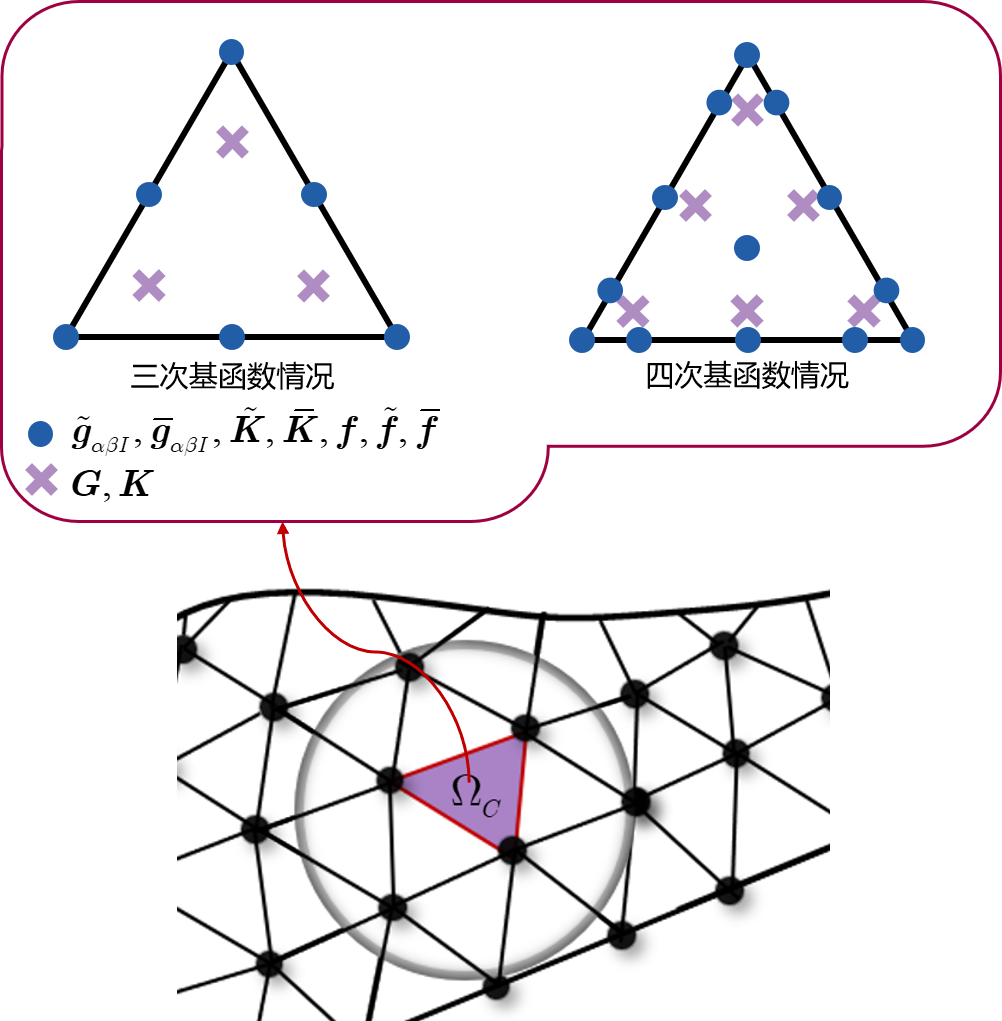
\includegraphics[scale=0.5]{figure/PHR/Pintegralscheme.png}
    \caption{优化的数值积分方案}\label{Pintegralscheme}
\end{figure}
\section{数值算例}
\subsection{分片实验}
关于薄板问题,采用二次、三次和四次高阶薄板分片实验验证采用传统高斯积分法和再生光滑梯度积分法的不同本质边界条件施加方法是否和二阶弹性力学问题相同
满足积分约束条件。此时分片实验考虑求解域为$\Omega=(0,1)\otimes(0,1)$的正方形薄板,求解域的四边施加本质边界条件。其分片实验的精确解如下:
\begin{equation}
\begin{split}
    w(\pmb{x})=\begin{cases}
        x_1^2+2x_1x_2\quad &\text{二次分片实验}\\
        x_1^3+2x_1^2x_2+3x_1x_2^2\quad &\text{三次分片实验}\\
        x_1^4+2x_1^3x_2+3x_1^2x_2^2+4x_1x_2^3\quad&\text{四次分片实验}
    \end{cases}
\end{split}
\end{equation}\par
如图所示(\ref{fenpian}),薄板问题的分片实验由49个无网格节点进行离散。针对三次基函数的无网格近似,采用二次和三次分片实验进行测试,核函数的相对影响域在三次基函数的情况下设为3.5;
而四次基函数的无网格近似采用三次和四次分片实验进行测试,核函数的相对影响域在四次基函数的情况下设为4.5。\par
\begin{figure}[H]
    \centering
    \includegraphics[scale=0.7]{figure/PHR/fenpian.png}
    \caption{分片实验无网格离散模型}\label{fenpian}
\end{figure}
为了更好的对比所提方法的计算精度,针对四阶薄板问题分别采用如下位移误差$L_2-\text{Error}$和能量误差$H_i-\text{Error}$进行分析:
\begin{equation}
\begin{split}
    &L_2-\text{Error}=\frac{\sqrt{\int_{\Omega}(w-w^h)^2d\Omega}}{\sqrt{\int_{\Omega}w^2d\Omega}}\\
    &H_i-\text{Error}=\frac{\sum_{j=0}^{i}\sqrt{\int_{\Omega}(w_{,\alpha_1\dotsb \alpha_j}-w_{,\alpha_1\dotsb \alpha_j})^2}d\Omega}{\sum_{j=0}^{i}\sqrt{\int_{\Omega}w_{,\alpha_1\dotsb \alpha_j}w_{,\alpha_1\dotsb \alpha_j}d\Omega}}
\end{split}
\end{equation}\par
针对薄板问题,三次基函数的求解计算时高斯积分法“GI”的求解域$\Omega$的积分采用13点高斯积分,边界$\Gamma$积分采用3点高斯积分;
四次基函数的求解计算时高斯积分法“GI”的求解域$\Omega$的积分采用16点高斯积分,边界$\Gamma$积分采用5点高斯积分;
再生光滑梯度积分法“RKGSI”计算时采用的积分点数和高斯积分法一致。三次和四次基函数的无网格分片试验结果如下表:
\newpage
\begin{table}[H]
    \caption{\textbf{三次基函数无网格法分片实验结果}}
    \centering\label{cubic}
   \begin{tabular}{ccccc}
   \toprule
    $\quad$&\multicolumn{2}{c}{二次分片实验}&\multicolumn{2}{c}{三次分片实验}\\
   \midrule
   &$L_2$-Error$\quad$&$H_2$-Error&$L_2$-Error$\quad$&$H_2$-Error\\
   \midrule
   GI-Penalty&$4.27\times10^{-2}$&$3.82\times10^{-1}$&$9.54\times10^{-2}$&$5.12\times10^{-1}$\\
   GI-Nitsche&$4.09\times10^{-2}$&$3.75\times10^{-1}$&$9.50\times10^{-2}$&$5.05\times10^{-1}$\\
  RKGSI-Penalty&$4.60\times10^{-2}$&$3.86\times10^{-1}$&$1.07\times10^{-1}$&$5.40\times10^{-1}$\\
  RKGSI-Nitsche&$5.67\times10^{-14}$&$2.18\times10^{-12}$&$5.21\times10^{-14}$&$1.20\times10^{-12}$\\
  RKGSI-HR&$5.58\times10^{-15}$&$4.56\times10^{-13}$&$3.66\times10^{-15}$&$2.70\times10^{-13}$\\
   \bottomrule
   \end{tabular}
   \end{table}
\begin{table}[H]
    \caption{\textbf{四次基函数无网格法分片实验结果}}
    \centering\label{quartic}
   \begin{tabular}{ccccc}
   \toprule
   $\quad$&\multicolumn{2}{c}{三次分片实验}&\multicolumn{2}{c}{四次分片实验}\\
   \midrule
   &$L_2$-Error$\quad$&$H_1$-Error&$L_2$-Error$\quad$&$H_1$-Error\\
   \midrule
   GI-Penalty&$1.08\times10^{-1}$&$5.44\times10^{-1}$&$1.84\times10^{-1}$&$6.32\times10^{-1}$\\
   GI-Nitsche&$1.07\times10^{-1}$&$5.45\times10^{-1}$&$1.84\times10^{-1}$&$6.34\times10^{-1}$\\
  RKGSI-Penalty&$1.06\times10^{-1}$&$5.40\times10^{-1}$&$1.84\times10^{-1}$&$6.26\times10^{-1}$\\
  RKGSI-Nitsche&$2.82\times10^{-13}$&$4.99\times10^{-12}$&$3.03\times10^{-13}$&$3.33\times10^{-12}$\\
  RKGSI-HR&$1.68\times10^{-14}$&$2.33\times10^{-12}$&$4.40\times10^{-14}$&$1.57\times10^{-12}$\\
\bottomrule
\end{tabular}
\end{table}\par
表(\ref{cubic})和表(\ref{quartic})分别表示具有三次、四次基函数无网格法的薄板分片试验结果,从表中可以明显的看出,由于缺乏变分一致性
传统高斯积分法“GI-Penalty”、“GI-Nitsche”和罚函数法“RKGSI-Penalty”都无法通过分片试验。只有满足变分一致性的再生光滑梯度积分法的“RKGSI-Nitsche”法和
本章提出的Hellinger-Ressiner变分原理的本质边界条件施加方案“RKGSI-HR”法可以通过分片试验,满足积分约束条件。
\subsection{简支方板问题}
如图(\ref{rectangular})所示,一简支方板的中性面区域为$\Omega=(0,1)\otimes(0,1)$,此时$\Omega$的长为$a=1$宽为$b=1$,材料系数分别为弯曲刚度$\bar{D}=1$、$\nu=0.3$。板面内分布如图所示纵向荷载:
\begin{equation}
\begin{split}
    \bar q=-\bar D(\frac{\pi^2}{a^2}+\frac{\pi^2}{b^2})sin(\frac{\pi}{a}x)sin(\frac{\pi}{b}y)
\end{split}
\end{equation}
该简支方板问题的精确解为:
\begin{equation}
\begin{split}
    w=-sin(\frac{\pi}{a}x)sin(\frac{\pi}{b}y)
\end{split}
\end{equation}
\begin{figure}[H]
\centering
    \includegraphics[scale=0.7]{figure/PHR/R/rectangular.png}
    \caption{简支方板问题模型}\label{rectangular}
\end{figure}
如图所示(\ref{rectangularmsh}),简支方板求解域采用均布的$11\times 11$、$21\times 21$、$41\times 41$、$81\times 81$的四个疏密不同的节点进行离散。
此时对于采用三次基函数的简支方板问题其相对影响域取为3.5,采用四次基函数时其相对影响域则取为4.5。\par

\begin{figure}[H]
\centering
      \includegraphics[scale=0.4]{figure/PHR/R/rectangularmsh.png}
    \caption{简支方板问题节点离散}\label{rectangularmsh}
\end{figure}
 图(\ref{RCLH})-图(\ref{RQLH})分别为简支方板问题在三次基函数和四次基函数时的位移误差和能量误差对比图。从图中可以明显看出即使采用高阶高斯积分法“GI”如三次基函数的13点高斯积分法和四次基函数的16点高斯积分,
计算精度都低于再生光滑梯度法“RKGSI”,并且和同样不满足变分一致性的罚函数法一样都无法达到理论误差收敛率。而“RKGSI-Nitsche”和“RKGSI-HR”法不管是在三次基函数还是四次基函数时都达到了误差收敛率。
图(\ref{RCcputime})-(\ref{RQcputime})是简支方板问题在三次基函数和四次基函数时分别计算节点数和与使用“GI”和“RKGSI”不同数值积分方法时的效率图。从整体来看采用“RKGSI”时的计算效率在三次基函数和四次基函数时都明显高于“GI”。  
% \begin{figure}[H]
%     \centering
%     \begin{subcaptiongroup}
%     \includegraphics[width=0.49\textwidth]{figure/PHR/R/CL2.png}
%     \phantomcaption\label{CL2}
%     \includegraphics[width=0.49\textwidth]{figure/PHR/R/CH1.png}
%     \phantomcaption\label{CH1}
%     \end{subcaptiongroup}
%     \begin{subcaptiongroup}
%     \includegraphics[width=0.49\textwidth]{figure/PHR/R/CH2.png}
%     \phantomcaption\label{CH2}
%     \includegraphics[width=0.49\textwidth]{figure/PHR/R/CH3.png}
%     \phantomcaption\label{CH3}
%     \end{subcaptiongroup}
% \caption{简支方板问题三次基函数误差对比:\subref{CL2} $L_2$误差;\subref{CH1} $H_1$;误差\subref{CH2};$H_2$误差;\subref{CH3} $H_3$误差}
% \label{RCLH}
% \end{figure}
% \newpage
% \begin{figure}[H]
%     \centering
%     \begin{subcaptiongroup}
%     \includegraphics[width=0.49\textwidth]{figure/PHR/R/QL2.png}
%     \phantomcaption\label{QL2}
%     \includegraphics[width=0.49\textwidth]{figure/PHR/R/QH1.png}
%     \phantomcaption\label{QH1}
%     \end{subcaptiongroup}
%     \begin{subcaptiongroup}
%     \includegraphics[width=0.49\textwidth]{figure/PHR/R/QH2.png}
%     \phantomcaption\label{QH2}
%     \includegraphics[width=0.49\textwidth]{figure/PHR/R/QH3.png}
%     \phantomcaption\label{QH3}
%     \end{subcaptiongroup}
% \caption{简支方板问题四次基函数误差对比:\subref{QL2} $L_2$误差;\subref{QH1} $H_1$误差;\subref{QH2};$H_2$误差;\subref{QH3} $H_3$误差}
% \label{RQLH}
% \end{figure}
% \begin{figure}[H]
%     \centering
%     \begin{subcaptiongroup}
%     \includegraphics[width=0.49\textwidth]{figure/PHR/R/Ccputime.png}
%     \phantomcaption\label{Ccputime}
%     \includegraphics[width=0.49\textwidth]{figure/PHR/R/Cefficiency.png}
%     \phantomcaption\label{Cefficiency}
%     \end{subcaptiongroup}
% \caption{简支方板问题三次基函数效率对比:\subref{Ccputime}计算时间与节点数的关系;\subref{Cefficiency}本质边界条件施加效率分析}
% \label{RCcputime}
% \end{figure}
% \newpage
% \begin{figure}[H]
%     \centering
%     \begin{subcaptiongroup}
%     \includegraphics[width=0.49\textwidth]{figure/PHR/R/Qcputime.png}
%     \phantomcaption\label{Qcputime}
%     \includegraphics[width=0.49\textwidth]{figure/PHR/R/Qefficiency.png}
%     \phantomcaption\label{Qefficiency}
%     \end{subcaptiongroup}
% \caption{简支方板问题四次基函数效率对比:\subref{Qcputime}计算时间与节点数的关系;\subref{Cefficiency}本质边界条件施加效率分析}
% \label{RQcputime}
% \end{figure}
\begin{figure}[H]
    \centering
    \includegraphics[scale=0.5]{figure/PHR/R/CL2.png}
    \caption{简支方板问题三次基函数$L_2$误差对比}\label{RCLH}
\end{figure}
\begin{figure}[H]
    \centering
    \includegraphics[scale=0.5]{figure/PHR/R/CH1.png}
    \caption{简支方板问题三次基函数$H_1$误差对比}
\end{figure}
\begin{figure}[H]
    \centering
    \includegraphics[scale=0.5]{figure/PHR/R/CH2.png}
    \caption{简支方板问题三次基函数$H_2$误差对比}
\end{figure}
\begin{figure}[H]
    \centering
    \includegraphics[scale=0.5]{figure/PHR/R/CH3.png}
    \caption{简支方板问题三次基函数$H_3$误差对比}
\end{figure}
\newpage
\begin{figure}[H]
    \centering
    \includegraphics[scale=0.5]{figure/PHR/R/QL2.png}
    \caption{简支方板问题四次基函数$L_2$误差对比}
\end{figure}
\begin{figure}[H]
    \centering
    \includegraphics[scale=0.5]{figure/PHR/R/QH1.png}
    \caption{简支方板问题四次基函数$H_1$误差对比}
\end{figure}
\newpage
\begin{figure}[H]
    \centering
    \includegraphics[scale=0.5]{figure/PHR/R/QH2.png}
    \caption{简支方板问题四次基函数$H_2$误差对比}
\end{figure}
\begin{figure}[H]
    \centering
    \includegraphics[scale=0.5]{figure/PHR/R/QH3.png}
    \caption{简支方板问题四次基函数$H_3$误差对比}\label{RQLH}
\end{figure}
\newpage
\begin{figure}[H]
    \centering
    \includegraphics[scale=0.5]{figure/PHR/R/Ccputime.png}
    \caption{简支方板问题三次基函数计算时间与节点数的关系}\label{RCcputime}
\end{figure}
\begin{figure}[H]
    \centering
    \includegraphics[scale=0.5]{figure/PHR/R/Cefficiency.png}
    \caption{简支方板问题三次基函数本质边界条件施加效率对比}
\end{figure}
\newpage
\begin{figure}[H]
    \centering
    \includegraphics[scale=0.5]{figure/PHR/R/Qcputime.png}
    \caption{简支方板问题四次基函数计算时间与节点数的关系}
\end{figure}
\begin{figure}[H]
    \centering
    \includegraphics[scale=0.5]{figure/PHR/R/Qefficiency.png}
    \caption{简支方板问题四次基函数本质边界条件施加效率对比}\label{RQcputime}
\end{figure}
图(\ref{calpha})、图(\ref{qalpha})是分别验证简支方板问题在三次基函数和四次基函数时带有人工经验参数的罚函数法和Nitsche法的敏感度分析。
从图中可以明显的看出,不同的经验参数对罚函数法的误差有着很大的影响,并且它的最优误差只在一小部分。
Nitsche法的最优误差的人工经验参数的范围比较大,但人工经验参数值的大小仍然会影响误差结果的变化,
并且随着网格的加密,人工经验参数的最优结果是在发生改变的。此时,提出的基于Hellinger-Reissner变分原理
中由于内嵌了本质边界条件,无需人工经验参数来满足正定性,相较于同样满足积分约束条件的“RKGSI-Nitsche”法,提出的“RKGSI-HR”法的不因人工参数值的变化影响最优误差。
% \begin{figure}[H]
%     \centering
%     \begin{subcaptiongroup}
%     \includegraphics[width=0.49\textwidth]{figure/PHR/R/calpha.png}
%     \phantomcaption\label{calpha}
%     \includegraphics[width=0.49\textwidth]{figure/PHR/R/qalpha.png}
%     \phantomcaption\label{qalpha}
%     \end{subcaptiongroup}
% \caption{人工参数$\alpha$敏感度分析:\subref{calpha}三次基函数;\subref{qalpha}四次基函数}
% \label{Ralpha}
% \end{figure}
% \newpage
\begin{figure}[H]
    \centering
    \includegraphics[scale=0.5]{figure/PHR/R/calpha.png}
    \caption{简支方板问题三次基函数人工参数$\alpha$敏感性分析}\label{calpha}
\end{figure}
\newpage
\begin{figure}[H]
    \centering
    \includegraphics[scale=0.5]{figure/PHR/R/qalpha.png}
    \caption{简支方板问题四次基函数人工参数$\alpha$敏感性分析}\label{qalpha}
\end{figure}
\subsection{简支等边三角形板问题}
一简支等边三角形板如图(\ref{triangular})所示,其中,三角形板的高为$a=10$,均布荷载作用在板面内为$\bar{q}=1$,材料系数分别为弯曲刚度$\bar{D}=1$、泊松比$\nu=0.3$。该简支三角形板的精确解为:
\begin{equation}
\begin{split}
    w=\frac{\bar q}{64a\bar D}[x^3-3y^3x-a(x^2+y^2)+\frac{4}{27}a^3](\frac{4}{9}a^2-x^2-y^2)
\end{split}
\end{equation}\par
如图(\ref{triangularmsh})所示,简支等边三角形板求解域分布采用均布离散的66、231、861和3321的四个疏密不同的节点进行离散。同样采用三次基函数时,简支等边三角形板问题的相对影响域取为3.5,四次基函数时其相对应影响域取为4.5进行数值分析。\par
\newpage
\begin{figure}[H]
    \centering
    \includegraphics[scale=0.7]{figure/PHR/T/triangular.png}
    \caption{简支等边三角形板问题模型}\label{triangular}
\end{figure}
\begin{figure}[H]
    \centering
    \includegraphics[scale=0.4]{figure/PHR/T/triangularmsh.png}
    \caption{简支等边三角形问题节点离散}\label{triangularmsh}
\end{figure}
图(\ref{TCLH})-图(\ref{TQLH})为简支等边三角形板问题分别在三次基函数和四次基函数的位移误差和能量误差对比图。从图中可以明显看出采用“RKGSI”得出的计算精度优于“GI”法。
并且不管是三次基函数还是四次基函数“RKGSI-Nitsche”、“RKGSI-HR”都能够达到理论误差收敛率,满足积分约束条件。
图(\ref{Tefficiency1})、图(\ref{Tefficiency2})是简支等边三角形板的薄板中面和本质边界条件施加效率分析图,从图中可以看出在薄板中面施加过程中,“RKGSI”所用的时间都明显少于“GI”;
而针对“RKGSI”在施加本质边界过程中计算形函数及梯度和组装相对应的刚度矩阵和力向量中可以明显看出“RKGSI-Nistche”法所用的时间明显多于“RKGSI-HR”和“RKGSI-Penalty”,
虽然“RKGSI-HR”和“RKGSI-Penalty”的计算效率相差不大,但“RKGSI-Penalty”由于不具有变分一致性无法达到理论误差收敛率。因此相较于传统的本质边界条件施加方法,
“RKGSI-HR”不仅满足积分约束条件能够达到理论误差收敛率,提高计算精度,在计算时间上也用时较短,有效提高计算效率。
图(\ref{TMxy})为简支等边三角形板问题的弯矩云图。从图中可以看出“RKGSI-HR”、“RKGSI-Nitsche”和“RKGSI-Penalty”和精确解之间非常一致,进一步验证了所提方法能够有效提高计算精度。
% \begin{figure}[H]
%     \centering
%     \begin{subcaptiongroup}
%     \includegraphics[width=0.49\textwidth]{figure/PHR/T/CL2.png}
%     \phantomcaption\label{CL2}
%     \includegraphics[width=0.49\textwidth]{figure/PHR/T/CH1.png}
%     \phantomcaption\label{CH1}
%     \end{subcaptiongroup}
%     \begin{subcaptiongroup}
%     \includegraphics[width=0.49\textwidth]{figure/PHR/T/CH2.png}
%     \phantomcaption\label{CH2}
%     \includegraphics[width=0.49\textwidth]{figure/PHR/T/CH3.png}
%     \phantomcaption\label{CH3}
%     \end{subcaptiongroup}
% \caption{简支等边三角形板问题三次基函数误差对比:\subref{CL2} $L_2$误差;\subref{CH1} $H_1$;误差\subref{CH2};$H_2$误差;\subref{CH3} $H_3$误差}
% \label{TCLH}
% \end{figure}
% \newpage
% \begin{figure}[H]
%     \centering
%     \begin{subcaptiongroup}
%     \includegraphics[width=0.49\textwidth]{figure/PHR/T/QL2.png}
%     \phantomcaption\label{QL2}
%     \includegraphics[width=0.49\textwidth]{figure/PHR/T/QH1.png}
%     \phantomcaption\label{QH1}
%     \end{subcaptiongroup}
%     \begin{subcaptiongroup}
%     \includegraphics[width=0.49\textwidth]{figure/PHR/T/QH2.png}
%     \phantomcaption\label{QH2}
%     \includegraphics[width=0.49\textwidth]{figure/PHR/T/QH3.png}
%     \phantomcaption\label{QH3}
%     \end{subcaptiongroup}
% \caption{简支等边三角形板问题四次基函数误差对比:\subref{QL2} $L_2$误差;\subref{QH1} $H_1$;误差\subref{QH2};$H_2$误差;\subref{QH3} $H_3$误差}
% \label{TQLH}
% \end{figure}
\begin{figure}[H]
    \centering
    \includegraphics[scale=0.5]{figure/PHR/T/CL2.png}
    \caption{简支等边三角形板问题三次基函数$L_2$误差对比}\label{TCLH}
\end{figure}
\begin{figure}[H]
    \centering
    \includegraphics[scale=0.5]{figure/PHR/T/CH1.png}
    \caption{简支等边三角形板问题三次基函数$H_1$误差对比}
\end{figure}
\newpage
\begin{figure}[H]
    \centering
    \includegraphics[scale=0.5]{figure/PHR/T/CH2.png}
    \caption{简支等边三角形板问题三次基函数$H_2$误差对比}
\end{figure}
\begin{figure}[H]
    \centering
    \includegraphics[scale=0.5]{figure/PHR/T/CH3.png}
    \caption{简支等边三角形板问题三次基函数$H_3$误差对比}
\end{figure}
\newpage
\begin{figure}[H]
    \centering
    \includegraphics[scale=0.5]{figure/PHR/T/QL2.png}
    \caption{简支等边三角形板问题四次基函数$L_2$误差对比}
\end{figure}
\begin{figure}[H]
    \centering
    \includegraphics[scale=0.5]{figure/PHR/T/QH1.png}
    \caption{简支等边三角形板问题四次基函数$H_1$误差对比}
\end{figure}
\newpage
\begin{figure}[H]
    \centering
    \includegraphics[scale=0.5]{figure/PHR/T/QH2.png}
    \caption{简支等边三角形板问题四次基函数$H_2$误差对比}
\end{figure}
\begin{figure}[H]
    \centering
    \includegraphics[scale=0.5]{figure/PHR/T/QH3.png}
    \caption{简支等边三角形板问题四次基函数$H_3$误差对比}\label{TQLH}
\end{figure}
\newpage
\begin{figure}[H]
    \centering
    \includegraphics[scale=0.5]{figure/PHR/T/Cefficiencyomega.png}
    \caption{简支等边三角形板问题薄板中面$\Omega$效率对比}\label{Tefficiency1}
\end{figure}
\begin{figure}[H]
    \centering
    \includegraphics[scale=0.5]{figure/PHR/T/Cefficiencygamma.png}
    \caption{简支等边三角形板问题本质边界条件$\Gamma_w,c_w$效率对比}\label{Tefficiency2}
\end{figure}
\newpage
% \begin{figure}[H]
%     \centering
%     \begin{subcaptiongroup}
%     \includegraphics[width=0.49\textwidth]{figure/PHR/T/Cefficiencyomega.png}
%     \phantomcaption\label{Cefficiencyomega}
%     \includegraphics[width=0.49\textwidth]{figure/PHR/T/Cefficiencygamma.png}
%     \phantomcaption\label{Cefficiencygamma}
%     \end{subcaptiongroup}
% \caption{简支等边三角形问题效率对比:\subref{Cefficiencyomega}薄板中面$\Omega$;\subref{Cefficiencygamma}本质边界条件$\Gamma_w,c_w$}
% \label{Tefficiency}
% \end{figure}
% \newpage
\begin{figure}[H]
\centering
    \includegraphics[scale=0.5]{figure/PHR/T/Mxy.png}
\caption{简支等边三角形板问题弯矩云图$\sigma_{xx}$应力云图}
\label{TMxy}
\end{figure}  
\subsection{简支环行板问题}
一简支环行板如图(\ref{annular})所示,其中内外径分别为$a=2$、$b=1$。在环行板的内外径边缘处分别施加弯矩$m_i=2$、$m_0=1$,
材料系数分别为抗弯刚度$\bar{D}=1$、泊松比为$\nu=0.3$。该简支环行板的精确解为:
\begin{equation}
\begin{split}
    w=\frac{(m_i-m_0)a^2b^2}{\bar D(1-\nu)(a^2-b^2)}ln\frac{r}{a}+\frac{m_ib^2-m_oa^2}{2\bar D(1+\nu)(a^2-b^2)}(r^2-a^2)
\end{split}
\end{equation}
其中:$r=\sqrt{x^2+y^2}$是点($x,y$)的极径。
\begin{figure}[H]
    \centering
    \includegraphics[scale=0.7]{figure/PHR/A/annular.png}
    \caption{简支环形板问题模型}\label{annular}
\end{figure}
如图(\ref{annularmsh})所示,简支环形问题求解域通过采用均布的153、561、2145和8385四个疏密不同的节点进行离散,
该简支环行板采用四次基函数,取相对影响域为4.5进行数值分析。\par
\begin{figure}[H]
    \centering
    \includegraphics[scale=0.4]{figure/PHR/A/annularmsh.png}
    \caption{简支环形板问题节点离散}\label{annularmsh}
\end{figure}
图(\ref{AQLH1})-图(\ref{AQLH2})为简支环行板问题的位移误差和能量误差对比图,从图中可以看出“RKGSI-HR”和“RKGSI-Nitsche”同样可以达到理论误差收敛率。
图(\ref{AQcputime})、图(\ref{AQefficiency})为简支环行板问题在计算时间节点数和施加不同本质边界条件上的效率对比,从图中可以看出采用“RKGSI”时的效率明显高于“GI”法,
与同样满足变分一致性的“RKGSI-Nitsche”法相比,“RKGSI-HR”法在施加过程中效率明显更高。
同样根据简支环行板的弯矩云图(\ref{AMxy})也可以更进一步说明在解决薄板问题上,基于Hellinger-Reissner变分原理的本质边界条件施加方法拥有着更高的计算精度。
在简支环行板问题中,存在两个人工参数影响计算精度。从图(\ref{Aalpha})中可以看出,随着节点数的变化“RKGSI-Nitsche”法和“RKGSI-Penalty”法在达到最优精度时的人工参数值也在发生变化。
而“RKGSI-HR”法中不涉及人工参数,因此随着节点数的增加,计算精度不会受到人工参数的影响,从而提高了一种更稳定和高效的计算方法。
% \begin{figure}[H]
%     \centering
%     \begin{subcaptiongroup}
%     \includegraphics[width=0.49\textwidth]{figure/PHR/A/QL2.png}
%     \phantomcaption\label{QL2}
%     \includegraphics[width=0.49\textwidth]{figure/PHR/A/QH1.png}
%     \phantomcaption\label{QH1}
%     \end{subcaptiongroup}
%     \begin{subcaptiongroup}
%     \includegraphics[width=0.49\textwidth]{figure/PHR/A/QH2.png}
%     \phantomcaption\label{QH2}
%     \includegraphics[width=0.49\textwidth]{figure/PHR/A/QH3.png}
%     \phantomcaption\label{QH3}
%     \end{subcaptiongroup}
% \caption{简支环行板问题四次基函数误差对比:\subref{QL2} $L_2$误差;\subref{QH1} $H_1$;误差\subref{QH2};$H_2$误差;\subref{QH3} $H_3$误差}
% \label{AQLH}
% \end{figure}
\begin{figure}[H]
    \centering
    \includegraphics[scale=0.5]{figure/PHR/A/QL2.png}
    \caption{简支环行板问题四次基函数$L_2$误差}\label{AQLH1}
\end{figure}
\begin{figure}[H]
    \centering
    \includegraphics[scale=0.5]{figure/PHR/A/QH1.png}
    \caption{简支环行板问题四次基函数$H_1$误差}
\end{figure}
\newpage
\begin{figure}[H]
    \centering
    \includegraphics[scale=0.5]{figure/PHR/A/QH2.png}
    \caption{简支环行板问题四次基函数$H_2$误差}
\end{figure}
\begin{figure}[H]
    \centering
    \includegraphics[scale=0.5]{figure/PHR/A/QH3.png}
    \caption{简支环行板问题四次基函数$H_3$误差}\label{AQLH2}
\end{figure}
\newpage
% \begin{figure}[H]
%     \centering
%     \begin{subcaptiongroup}
%     \includegraphics[width=0.49\textwidth]{figure/PHR/A/Qcputime.png}
%     \phantomcaption\label{Qcputime}
%     \includegraphics[width=0.49\textwidth]{figure/PHR/A/Qefficiency.png}
%     \phantomcaption\label{Qefficiency}
%     \end{subcaptiongroup}
% \caption{简支环形板问题四次基函数效率对比:\subref{Qcputime}计算时间与节点数的关系;\subref{Cefficiency}本质边界条件施加效率分析}
% \label{AQcputime}
% \end{figure}
\begin{figure}[H]
    \centering
    \includegraphics[scale=0.5]{figure/PHR/A/Qcputime.png}
    \caption{简支环行板问题四次基函数计算时间与节点数对比}\label{AQcputime}
\end{figure}
\begin{figure}[H]
    \centering
    \includegraphics[scale=0.5]{figure/PHR/A/Qefficiency.png}
    \caption{简支环行板问题四次基函数本质边界条件施加效率分析}\label{AQefficiency}
\end{figure}
\newpage
\begin{figure}[H]
    \centering
    \includegraphics[scale=0.5]{figure/PHR/A/Mxy.png}
    \caption{简支环形板问题弯矩云图}\label{AMxy}
\end{figure}
\begin{figure}[H]
    \centering
    \includegraphics[scale=0.5]{figure/PHR/A/alpha.png}
    \caption{简支环形板问题人工参数敏感性分析}\label{Aalpha}
\end{figure}
\section{小结}
本章进一步介绍了基于Hellinger-Reissner变分原理的变分一致性本质边界条件施加方法,用于求解四阶薄板问题。
该方法通过采用混合离散近似Hellinger-Reissner变分原理弱形式中的挠度和弯矩,实现了满足积分约束条件用于求解高阶薄板问题的一种本质边界条件施加方法。
其中,在离散平衡控制方程中,采用传统无网格形函数对挠度进行离散,弯矩则在每个背景积分单元上以再生光滑梯度独立逼近。
通过采用再生光滑梯度积分法,该方法内嵌了局部积分约束条件,因此严格满足了每个积分单元的变分一致性。此外,由于二阶光滑梯度的计算只涉及无网格形函数及其一阶导数,有效的提高了计算效率。 
之后通过典型的数值算例进一步表明所提方法基于Hellinger-Reissner变分原理无网格薄板公式在满足变分一致性,计算精度以及计算效率方面优于采用传统高斯积分法的Nitsche法、罚函数法以及采用再生光滑梯度积分法的Nitsche法,罚函数法。
基于Hellinger-Reissner变分原理的变分一致性本质边界条件施加方法在解决薄板问题上提供了一种高效精确的边界条件施加方法。






% \chapter{TADAS阻尼器}
在本章中对工程实际应用中常见的三角形板(TADAS)阻尼器进行介绍,随后通过数值建模对其进行数值分析,详细对比使用罚函数法、Nitsche法和HR法的位移云图,证明所提方法在解决工程实践应用问题具有一定的优势。
\section{TADAS阻尼器}
在建筑和工程结构中,振动是一个常见的问题,其可能会导致结构的疲劳破坏等问题,传统方法中通过采用增加结构的刚度或使用液体阻尼器、摩擦阻尼器减小结构的振动响应,然而在传统方法中或多或少的存在有效性不高,经济适用性低等问题。
为了克服传统方法的限制,三角板减振刚度阻尼器被引入(TADAS),TADAS阻尼器是一种基于能量耗散原理的被动控制装置,通过在结构中引入附加的阻尼力来吸收和耗散结构的振动能量,能够有效地减小结构地的振动幅值和振动周期,从而显著改善结构的振动响应,
并且TADAS阻尼器的设计相对简单,通常由一块或多块金属材料制成,安装简易、价格低廉,是一种在结构工程中广泛应用于减震和控制结构的被动控制装置。\par
图(\ref{TADAS1})为一个带有TADAS阻尼器的实验装置\textsuperscript{\cite{mohammadi2017,kim2016}},为常在道路、住房和城市中心建造的一层框架大比例模型,
该框架高3米,跨度4米,框架柱采用标准的双IPE180型钢材,梁的工字截面由三块4000*200*12mm的钢板连续焊接而成。支撑体系统一采用双100*100*20mm角度,柱基座使用销连接。
如图(\ref{TADAS2})所示,TADAS阻尼器中的三角形板的上端设为简支固定,下端施加$P=100000$的力。三角形钢板的材料系数为杨氏模量$E=2\times 10^{11}$、泊松比$\nu=0.3$。
\begin{figure}[H]
    \centering
    \includegraphics[scale=0.4]{figure/TADAS/1.png}
    \caption{实验装置示意图}\label{TADAS1}
\end{figure}
\begin{figure}[H]
    \centering
    \begin{subcaptiongroup}
            \includegraphics[width=0.69\textwidth]{figure/TADAS/2.png}
            \phantomcaption\label{TADAS2}
            \includegraphics[width=0.29\textwidth]{figure/TADAS/3.png}
            \phantomcaption\label{TADAS3}
            \end{subcaptiongroup}
        \caption{TADAS阻尼器示意图:\subref{TADAS2} 钢板焊接TADAS装置详图;\subref{TADAS3} 三角形钢板横截面图}
    \label{TADAS2}
\end{figure}
图(\ref{TADAS4})为TADAS阻尼器三角形板的位移应力云图,从图中可以看出所提方法“HR”法的计算结果与常见解决薄板实际应用问题的方法“Nitsche”法和罚函数法具有几乎相同的位移结果,说明我们所提出的新方法能够解决工程实践应用薄板问题。
\begin{figure}[H]
    \centering
    \includegraphics[scale=0.5]{figure/TADAS/4.png}
    \caption{TADAS阻尼器位移云图}\label{TADAS4}
\end{figure}
\section{小结}
本章首先对TADAS阻尼器的优点进行详细介绍,随后对一个一层框架大比例模型中带有TADAS阻尼器进行数值分析,通过采用不同的本质边界条件施加方法-罚函数法、Nitsche法和本论文所提方法HR法得到的位移云图进行分析,
得出基于Hellinger-Reissner变分原理的变分一致性伽辽金无网格法能够有效处理解决工程实际中的薄板模型,为薄板问题的工程数值分析提供了一种新思路。



\chapter{结论与展望}
\section{结论}
本文研究以Hellinger-Reissner变分原理为基础,依托于Hellinger-Reissner原理内嵌本质边界条件的特点,完善了缺乏完备理论基础的再生光滑梯度数值分析方法,为具有变分一致性的无网格分析方法提供了新思路,提出了一种具有高效、鲁棒的具有变分一致性的本质边界施加方案的新方法,能够有效提高传统无网格法的计算精度和效率。
具体结论如下:
\par
(1)以Hellinger-Reissner变分原理为基础,提出了一种满足积分约束条件的变分一致高效本质边界条件施加方法。该方法采用混合离散近似Hellinger-Reissner变分原理弱形式中位移和应力,
其中位移采用传统无网格形函数进行离散,而应力则在每个背景积分域上近似为对应阶次的多项式,满足局部的变分一致性。通过Hellinger-Reissner变分原理完善变分一致型伽辽金无网格数值积分方法的基础理论框架。
\par
(2)在Hellinger-Reissner变分原理的框架下,该方法的离散平衡方程中具有与传统Nitsche法相类似的表达式,可视为与再生光滑梯度积分法相配套的新型Nitsche法。
与传统Nitsche法相比,所提方法的修正变分项采用传统无网格形函数和再生光滑梯度进行混合离散,在保证了变分一致性的同时避免了复杂耗时的形函数导数计算,明显提高了计算效率;
而对于Nitsche法中的稳定项则直接源于Hellinger-Reissner变分原理弱形式中,无需额外增加稳定项,更重要的是稳定项中不包含任何人工参数,有效消除了Nitsche法中的人工参数依赖性。
在该论文中通过对弹性力学问题典型算例和薄板问题典型算例系统的验证了所提方法基于Hellinger-Reissner变分原理施加本质边界条件方法的变分一致性、计算精度和计算效率。
\section{展望}
本文仅是对弹性力学问题和薄板问题的典型算例进行验证所提方法的变分一致性、计算精度和计算效率,在本论文的典型算例中均是属于静力学问题,于是后续的研究工作有以下两点考虑:\par
(1)研究更为复杂的壳体问题基于Hellinger-Reissner变分原理的变分一致型伽辽金无网格法的变分一致性、计算精度和计算效率。本论文着重探讨基于Kirchhoff薄板假设理论进行推导,所以后续可以研究无法忽略剪切变形的壳体问题。\par
(2)研究动力学问题的算例在基于Hellinger-Reissner变分原理的挠度、频散特性。本论文着重探讨的算例验证均是属于静力学问题,所以后续研究可以探讨关于动力学的算例问题进一步验证所提方法的计算效果。



% \chapter{text}
\begin{figure}[H]
    \centering
    \includegraphics[scale=0.7]{figure/PHR/A/Mxy.png}
    \caption{简支环形板问题弯矩云图}\label{AMxy}
\end{figure}
\begin{figure}[H]
    \centering
        \includegraphics[scale=0.7]{figure/PHR/T/Mxy.png}
    \caption{简支等边三角形板问题弯矩云图$\sigma_{xx}$应力云图}
    \label{TMxy}
    \end{figure}  
    \begin{figure}[H]
        \centering
        \includegraphics[scale=1.0]{figure/PHR/A/alpha.png}
        \caption{简支环形板问题人工参数敏感性分析}\label{Aalpha}
    \end{figure}








\setcounter{equation}{0}
\renewcommand\theequation{A.\arabic{equation}}
\addcontentsline{toc}{chapter}{附录A:弹性力学问题HR变分原理的本质边界条件施加方法推导过程}
\appendix
\renewcommand{\appendixname}{Appendix~\Alph{chapter}}
\chapter*{附录A:弹性力学问题HR变分原理的本质边界条件施加方法推导过程}\label{A}
通过引入式(\ref{g1})、(\ref{case1})对式(\ref{inference})中的第一项进行推导得到:
\begin{equation}\label{CH4-K}
\begin{split}
    &\sum_{C=1}^{N\!C}\tilde{\pmb g}^T_{jI}C_{ijkl}\pmb{G}^{-1}\tilde{\pmb g}_{kJ}
=\sum_{C=1}^{N\!C}\tilde{\pmb g}^T_{jI}C_{ijkl}\pmb{G}^{-1}\pmb{G}\pmb{G}^{-1}\tilde{\pmb g}_{kJ}\\
&=\sum_{C=1}^{N\!C}\int_{\Omega_C}\tilde{\pmb g}_{jI}^T\pmb{G}^{-1}\pmb{p}^{[p-1]}(\pmb x)C_{ijkl}\pmb{p}^{[p-1]T}(\pmb{x})\pmb{G}^{-1}\tilde{\pmb g}_{kJ}d\Omega\\
&=\sum_{C=1}^{N\!C}\int_{\Omega_C}\tilde{\Psi}_{I,j}C_{ijkl}\tilde{\Psi}_{I,k}d\Omega\\
&=\sum_{C=1}^{N\!C}\int_{\Omega_C}\delta\tilde{\varepsilon}_{ij}^hC_{ijkl}\tilde{\varepsilon}_{kl}^hd\Omega\\
&=\int_{\Omega}\tilde{\pmb{B}}_I^T\pmb{D}\tilde{\pmb{B}}_Jd\Omega\\
&=\pmb{K}
\end{split}
\end{equation}
通过引入式(\ref{g3})、(\ref{case1})、(\ref{CH4-ui})对式(\ref{inference})中的第二、三项进行推导得到:
\begin{equation}\label{CH4-tildeK}
\begin{split}
    &-\sum_{C=1}^{N\!C}C_{ijkl}(\bar{\pmb g}_{jI}^T\pmb{G}^{-1}\tilde{\pmb g}_{kJ}+\tilde{\pmb g}_{jI}^T\pmb{G}^{-1}\bar{\pmb g}_{kJ})\\
    &=-\sum_{C=1}^{N\!C}(\int_{\Gamma^g\cap\partial\Omega_C}\Psi_In_jC_{ijkl}\pmb{p}^{[p-1]}\pmb{G}^{-1}\tilde{\pmb g}_{kJ}d\Gamma
    +\int_{\Gamma^g\cap\partial\Omega_C}C_{ijkl}\pmb{p}^{[p-1]}\pmb{G}^{-1}\tilde{\pmb g}_{jI}n_k\Psi_Jd\Gamma)\\
    &=-\sum_{C=1}^{N\!C}(\int_{\Gamma^g\cap\partial\Omega_C}\Psi_In_jC_{ijkl}\tilde{\Psi}_{J,k}d\Gamma
    +\int_{\Gamma^g\cap\partial\Omega_C}C_{ijkl}\sum_{J=1}^{N\!P}\tilde{\Psi}_{I,j}\delta d_{iI}n_k\sum_{I=1}^{N\!P}\Psi_Jd\Gamma)\\
    &=-\sum_{C=1}^{N\!C}(\int_{\Gamma^g\cap\partial\Omega}\delta u_i^hn_jC_{ijkl}\tilde{\varepsilon}_{kl}^hd\Gamma+\int_{\Gamma^g\cap\partial\Omega_C}\delta\tilde{\varepsilon}_{ij}^hC_{ijkl}n_ku^h_ld\Gamma)\\
    &=-(\int_{\Gamma^g}\Psi_I\pmb{N}\pmb{D}\tilde{\pmb{B}}_Jd\Gamma+\int_{\Gamma^g}\tilde{\pmb{B}}_I^T\pmb{D}\pmb{N}^T\Psi_Jd\Gamma)\\
    &=\tilde{\pmb{K}}
\end{split}
\end{equation}
通过引入式(\ref{g3})、(\ref{case2})对式(\ref{inference})中的第四项进行推导得到:
\begin{equation}\label{CH4-barK}
\begin{split}
    &\sum_{C=1}^{N\!C}C_{ijkl}\bar{\pmb g}^T_{jI}\pmb{G}^{-1}\bar{\pmb g}_{kJ}\\
    &=\sum_{C=1}^{N\!C}\int_{\Gamma^g\cap\partial\Omega_C}C_{ijkl}\bar{\pmb g}_{jI}^T\pmb{G}^{-1}\pmb{p}^{[p-1]}\Psi_Jn_kd\Gamma\\
    &=\sum_{C=1}^{N\!C}\int_{\Gamma^g\cap\partial\Omega_C}C_{ijkl}\bar{\Psi}_{I,j}n_k\Psi_{J}d\Gamma\\
    &=\sum_{C=1}^{N\!C}\int_{\Gamma^g\cap\partial\Omega_C}C_{ijkl}\delta\bar{\varepsilon}_{ij}^hn_ku_ld\Gamma\\
    &=\delta\pmb{d}_I^T\int_{\Gamma^g\cap\partial\Omega_C}\bar{\pmb{B}}_I^T\pmb{D}\pmb{N}^T\Psi_Jd\Gamma\\
    &=\bar{\pmb{K}}
\end{split}
\end{equation}
通过引入式(\ref{g4})、(\ref{case1})对式(\ref{inference})中的第五项进行推导得到:
\begin{equation}\label{CH4-tildef}
\begin{split}
    &-\sum_{C=1}^{N\!C}C_{ijkl}\tilde{\pmb g}^T_{jI}\pmb{G}^{-1}\hat{\pmb g}_{kl}\\
    &=-\sum_{C=1}^{N\!C}C_{ijkl}\tilde{\pmb g}^T_{jI}\pmb{G}^{-1}\int_{\Gamma^g\cap\partial\Omega_C}\pmb{p}^{[p-1]}n_lg_kd\Gamma\\
    &=-\sum_{C=1}^{N\!C}\int_{\Gamma^g\cap\partial\Omega_C}C_{ijkl}\tilde{\Psi}_{I,j}n_lg_kd\Gamma\\
    &=-\sum_{C=1}^{N\!C}\int_{\Gamma^g\cap\partial\Omega_C}C_{ijkl}\delta\tilde{\varepsilon}_{ij}^hn_lg_kd\Gamma\\
    &=-\int_{\Gamma^g\cap\partial\Omega_C}\tilde{\pmb{B}}_I^T\pmb{D}\pmb{N}^T\pmb{g}d\Gamma\\
    &=\tilde{\pmb f}
\end{split}
\end{equation}
通过引入式(\ref{g4})、(\ref{case2})对式(\ref{inference})中的第六项进行推导得到:
\begin{equation}\label{CH4-barf}
\begin{split}
    &\sum_{C=1}^{N\!C}C_{ijkl}\bar{\pmb g}^T_{jI}\pmb{G}^{-1}\hat{\pmb g}_{kl}\\
    &=\sum_{C=1}^{N\!C}C_{ijkl}\bar{\pmb g}^T_{jI}\pmb{G}^{-1}\int_{\Gamma^g\cap\partial\Omega_C}\pmb{p}^{[p-1]}n_lg_kd\Gamma\\
    &=\sum_{C=1}^{N\!C}\int_{\Gamma^g\cap\partial\Omega_C}C_{ijkl}\bar{\Psi}_{I,j}n_lg_kd\Gamma\\
    &=\sum_{C=1}^{N\!C}\int_{\Gamma^g\cap\partial\Omega_C}C_{ijkl}\delta\bar{\varepsilon}_{ij}^hn_lg_kd\Gamma\\
    &=\int_{\Gamma^g\cap\partial\Omega_C}\bar{\pmb{B}}_I^T\pmb{D}\pmb{N}^T\pmb{g}d\Gamma\\
    &=\bar{\pmb f}
\end{split}
\end{equation}


\addcontentsline{toc}{chapter}{附录B:薄板问题HR变分原理的本质边界条件施加方法推导过程}
\appendix
\renewcommand{\appendixname}{Appendix~\Alph{chapter}}
\chapter{薄板问题HR变分原理的本质边界条件施加方法推导过程}\label{B}
% \addcontentsline{toc}{chapter}{附录B:薄板问题HR变分原理的本质边界条件施加方法推导过程}
通过引入式(\ref{PG})、(\ref{PTPSI})对式(\ref{Pzuzhuang})中的第一项进行推导可以得到:
\begin{equation}
\begin{split}
    &\sum_{C=1}^{N\!C}D_{\alpha\beta\gamma\eta}\tilde{\pmb g}_{\alpha\beta I}^T\pmb G^{-1}\tilde{\pmb g}_{\gamma\eta J}\\
    &=\sum_{C=1}^{N\!C}D_{\alpha\beta\gamma\eta}\tilde{\pmb g}_{\alpha\beta I}^T\pmb G^{-1}\int_{\Omega_C}\pmb{p}^{[p-2]}\pmb{p}^{[p-2]T}d\Omega\pmb G^{-1}\tilde{\pmb g}_{\gamma\eta J}\\
    &=\sum_{C=1}^{N\!C}D_{\alpha\beta\gamma\eta}\int_{\Omega_C}\tilde{\pmb g}_{\alpha\beta I}^T\pmb G^{-1}\pmb{p}^{[p-2]}\pmb{p}^{[p-2]T}\pmb G^{-1}\tilde{\pmb g}_{\gamma\eta J}d\Omega \\
    &=\int_{\Omega}\tilde{\Psi}_{I,\alpha\beta}D_{\alpha\beta\gamma\eta}\tilde{\Psi}_{J,\gamma\eta}d\Omega \\
    &=\pmb{K}
\end{split}
\end{equation}
\newpage
通过引入式(\ref{PTPSI})、(\ref{MVP1})对式(\ref{Pzuzhuang})中的第二项进行推导可以得到:
\begin{equation}
\begin{split}
    &-\sum_{C=1}^{N\!C}D_{\alpha\beta\gamma\eta}(\bar{\pmb g}_{\alpha\beta I}^T\pmb G^{-1}\tilde{\pmb g}_{\gamma\eta J}+\tilde{\pmb g}_{\alpha\beta I}^T\pmb G^{-1}\tilde{\pmb g}_{\gamma\eta J})\\
    &=\sum_{C=1}^{N\!C}D_{\alpha\beta\gamma\eta}\int_{{\Gamma_w}\cap{\Gamma_C}}\Psi_I(n_{\alpha}
    \pmb{p}^{[p-2]T}_{,\beta}\pmb G^{-1}\tilde{\pmb g}_{\gamma\eta J}+\pmb{p}^{[p-2]T}_{,\xi}\pmb G^{-1}\tilde{\pmb g}_{\gamma\eta J}s_{\alpha}n_{\beta}s_{\xi})d\Gamma\\
    &+\sum_{C=1}^{N\!C}D_{\alpha\beta\gamma\eta}\int_{{\Gamma_w}\cap{\Gamma_C}}(n_{\gamma}
    \tilde{\pmb g}_{\alpha\beta I}^T\pmb G^{-1}\pmb{p}^{[p-2]}_{,\eta}+\tilde{\pmb g}_{\alpha\beta I}^T
    \pmb G^{-1}\pmb{p}^{[p-2]}_{,\xi}s_{\gamma}n_{\eta}s_{\xi})\Psi_Jd\Gamma\\
    &-\sum_{C=1}^{N\!C}D_{\alpha\beta\gamma\eta}\int_{{\Gamma_{\theta}}\cap{\Gamma_C}}\Psi_{I,n}
    \pmb{p}^{[p-2]T}\pmb G^{-1}\tilde{\pmb g}_{\gamma\eta J}n_{\alpha}n_{\beta}d\Gamma
    -\sum_{C=1}^{N\!C}D_{\alpha\beta\gamma\eta}\int_{{\Gamma_{\theta}}\cap{\Gamma_C}}
    \tilde{\pmb g}_{\alpha\beta I}^T\pmb G^{-1}\pmb{p}^{[p-2]}n_{\gamma}n_{\eta}\Psi_{J,n}d\Gamma\\
    &-\sum_{C=1}^{N\!C}D_{\alpha\beta\gamma\eta}[[\Psi_I\pmb{p}^{[p-2]T}\pmb G^{-1}\tilde{\pmb g}_{\gamma\eta J}n_{\alpha}s_{\beta}]]_{x\in{c_w}\cap{c_C}}
    -\sum_{C=1}^{N\!C}D_{\alpha\beta\gamma\eta}[[\tilde{\pmb g}_{\alpha\beta I}^T\pmb G^{-1}\pmb{p}^{[p-2]}n_{\gamma}s_{\eta}\Psi_J]]_{x\in{c_w}\cap{c_C}}\\
    &=-\sum_{C=1}^{N\!C}\int_{{\Gamma_w}\cap{\Gamma_C}}\Psi_I(-D_{\alpha\beta\gamma\eta}(n_{\alpha}\frac{\partial}{\partial x_{\beta}}+s_{\alpha}n_{\beta}s_{\xi}\frac{\partial}{\partial x_{\xi}}))\tilde{\Psi}_{J,\gamma\eta}d\Gamma\\
    &-\sum_{C=1}^{N\!C}\int_{{\Gamma_w}\cap{\Gamma_C}}(-D_{\alpha\beta\gamma\eta}(n_{\gamma}\frac{\partial}{\partial x_{\eta}}+s_{\gamma}n_{\eta}s_{\xi}\frac{\partial}{\partial x_{\xi}}))\tilde{\Psi}_{I,\alpha\beta}\Psi_Jd\Gamma\\
    &+\sum_{C=1}^{N\!C}\int_{{\Gamma_{\theta}}\cap{\Gamma_C}}\Psi_{I,n}(-D_{\alpha\beta\gamma\eta}n_{\alpha}n_{\beta})\tilde{\Psi}_{J,\gamma\eta}d\Gamma
    +\sum_{C=1}^{N\!C}\int_{{\Gamma_{\theta}}\cap{\Gamma_C}}(-D_{\alpha\beta\gamma\eta}n_{\gamma}n_{\eta})\tilde{\Psi}_{I,\alpha\beta}\Psi_{J,n}d\Gamma\\
    &+\sum_{C=1}^{N\!C}[[\Psi_I(-D_{\alpha\beta\gamma\eta}n_{\gamma}s_{\eta})\tilde{\Psi}_{J,\gamma\eta}]]_{x\in{c_w}\cap{c_C}}+\sum_{C=1}^{N\!C}[[(-D_{\alpha\beta\gamma\eta}n_{\gamma}s_{\eta})\tilde{\Psi}_{I,\alpha\beta}\Psi_J]]_{x\in{c_w}\cap{c_C}}\\
    &=-\int_{\Gamma_w}\Psi_I\mathcal{V}_{\alpha\beta}\tilde{\Psi}_{J,\alpha\beta}d\Gamma+\int_{\Gamma_{\theta}}\Psi_{I,n}\mathcal{M}_{\alpha\beta}\tilde{\Psi}_{J,\alpha\beta}d\Gamma+[[\Psi_I\mathcal{P}_{\alpha\beta}\tilde{\Psi}_{J,\alpha\beta}]]_{x\in{c_w}}\\
    &-\int_{\Gamma_w}\mathcal{V}_{\alpha\beta}\tilde{\Psi}_{I,\alpha\beta}\Psi_Jd\Gamma+\int_{\Gamma_{\theta}}\mathcal{M}_{\alpha\beta}\tilde{\Psi}_{I,\alpha\beta}\Psi_{J,n}d\Gamma+[[\mathcal{P}_{\alpha\beta}\tilde{\Psi}_{I,\alpha\beta}\Psi_J]]_{x\in{c_w}}\\
    &=\tilde{\pmb K}
\end{split}
\end{equation}
\newpage
通过引入式(\ref{PBPSI})、(\ref{MVP1})对式(\ref{Pzuzhuang})中的第三项进行推导可以得到:
\begin{equation}
\begin{split}
    &\sum_{C=1}^{N\!C}D_{\alpha\beta\gamma\eta}\bar{\pmb g}_{\alpha\beta I}^T\pmb G^{-1}\tilde{\pmb g}_{\gamma\eta J}\\
    &=\sum_{C=1}^{N\!C}D_{\alpha\beta\gamma\eta}\int_{{\Gamma_w}\cap{\Gamma_C}}(n_{\gamma}
    \bar{\pmb g}_{\alpha\beta I}^T\pmb G^{-1}\pmb{p}^{[p-2]}_{,\eta}+\tilde{\pmb g}_{\alpha\beta I}^T
    \pmb G^{-1}\pmb{p}^{[p-2]}_{,\xi}s_{\gamma}n_{\eta}s_{\xi})\Psi_Jd\Gamma\\
    &-\sum_{C=1}^{N\!C}D_{\alpha\beta\gamma\eta}\int_{{\Gamma_{\theta}}\cap{\Gamma_C}}
    \bar{\pmb g}_{\alpha\beta I}^T\pmb G^{-1}\pmb{p}^{[p-2]}n_{\gamma}n_{
    \eta}\Psi_{J,n}d\Gamma
    -\sum_{C=1}^{N\!C}D_{\alpha\beta\gamma\eta}[[\bar{\pmb g}_{\alpha\beta I}^T\pmb G^{-1}\pmb{p}^{[p-2]}n_{\gamma}s_{\eta}\Psi_J]]_{x\in{c_w}\cap{c_C}}\\
    &=\sum_{C=1}^{N\!C}\int_{{\Gamma_w}\cap{\Gamma_C}}(-D_{\alpha\beta\gamma\eta}(n_{\gamma}\frac{\partial}{\partial x_{\eta}}+s_{\gamma}n_{\eta}s_{\xi}\frac{\partial}{\partial x_{\xi}}))\bar{\Psi}_{I,\alpha\beta}\Psi_Jd\Gamma\\
    &-\sum_{C=1}^{N\!C}\int_{{\Gamma_{\theta}}\cap{\Gamma_C}}(-D_{\alpha\beta\gamma\eta}n_{\gamma}n_{\eta})\bar{\Psi}_{I,\alpha\beta}\Psi_{J,n}d\Gamma
    -[[(-D_{\alpha\beta\gamma\eta}n_{\gamma}s_{\eta})\bar{\Psi}_{I,\alpha\beta}\Psi_J]]_{x\in{c_w}\cap{c_C}}\\
    &=\int_{\Gamma_w}\mathcal{V}_{\alpha\beta}\bar{\Psi}_{I,\alpha\beta}\Psi_Jd\Gamma-\int_{\Gamma_{\theta}}\mathcal{M}_{\alpha\beta}\bar{\Psi}_{I,\alpha\beta}\Psi_{J,n}d\Gamma+[[\mathcal{P}_{\alpha\beta}\bar{\Psi}_{I,\alpha\beta}\Psi_J]]_{x\in{c_w}}\\
    &=\bar{\pmb K}
\end{split}
\end{equation}
通过引入式(\ref{PTPSI})、(\ref{MVP1})对式(\ref{Pzuzhuang})中的第四项进行推导可以得到:
\begin{equation}
\begin{split}
    &-\sum_{C=1}^{N\!C}D_{\alpha\beta\gamma\eta}\tilde{\pmb g}^T_{\alpha\beta I}\pmb G^{-1}\hat{\pmb g}_{\gamma\eta}\\
    &=\sum_{C=1}^{N\!C}D_{\alpha\beta\gamma\eta}\int_{{\Gamma_w}\cap{\Gamma_C}}(n_{\gamma}
    \tilde{\pmb g}_{\alpha\beta I}^T\pmb G^{-1}\pmb{p}^{[p-2]}_{,\eta}+\tilde{\pmb g}_{\alpha\beta I}^T
    \pmb G^{-1}\pmb{p}^{[p-2]}_{,\xi}s_{\gamma}n_{\eta}s_{\xi})\bar{w}d\Gamma\\
    &-\sum_{C=1}^{N\!C}D_{\alpha\beta\gamma\eta}\int_{{\Gamma_{\theta}}\cap{\Gamma_{C}}}\tilde{\pmb g}^T_{\alpha\beta I}\pmb G^{-1}\pmb{p}^{[p-2]}n_{\gamma}n_{\eta}\bar{\theta}_nd\Gamma-[[\tilde{\pmb g}_{\alpha\beta I}\pmb G^{-1}\pmb{p}^{[p-2]}n_{\gamma}s_{\eta}\bar{w}]]_{x\in{c_w}\cap{c_C}}\\
    &=-\sum_{C=1}^{N\!C}\int_{{\Gamma_w}\cap{\Gamma_C}}(-D_{\alpha\beta\gamma\eta}(n_{\gamma}\frac{\partial}{\partial x_{\eta}}+s_{\gamma}n_{\eta}s_{\xi}\frac{\partial}{\partial x_{\xi}}))\tilde{\Psi}_{I,\alpha\beta}\bar{w}d\Gamma\\
    &+\sum_{C=1}^{N\!C}\int_{{\Gamma_{\theta}}\cap{\Gamma_C}}(-D_{\alpha\beta\gamma\eta}n_{\gamma}n_{\eta})\tilde{\Psi}_{I,\alpha\beta}\bar{\theta}_{\pmb n}d\Gamma-[[(-D_{\alpha\beta\gamma\eta}n_{\gamma}s_{\eta}\tilde{\Psi}_{I,\alpha\beta}\bar{w})]]_{x\in{c_w}\cap{c_C}}\\
    &=\int_{\Gamma_w}\mathcal{V}_{\alpha\beta}\tilde{\Psi}_{I,\alpha\beta}\bar{w}d\Gamma+\int_{\Gamma_{\theta}}\mathcal{M}_{\alpha\beta}\tilde{\Psi}_{I,\alpha\beta}\bar{\theta}_{\pmb n}d\Gamma+[[\mathcal{P}_{\alpha\beta}\tilde{\Psi}_{I,\alpha\beta}\bar{w}]]_{x\in{c_w}}\\
    &=\tilde{\pmb f}
\end{split}
\end{equation}
通过引入式(\ref{PBPSI})、(\ref{MVP1})对式(\ref{Pzuzhuang})中的第五项进行推导可以得到:
\begin{equation}
 \begin{split}
    &-\sum_{C=1}^{N\!C}D_{\alpha\beta\gamma\eta}\bar{\pmb g}_{\alpha\beta I}^T\pmb G^{-1}\hat{\pmb g}_{\gamma\eta }\\
    &=\sum_{C=1}^{N\!C}D_{\alpha\beta\gamma\eta}\int_{{\Gamma_w}\cap{\Gamma_C}}(n_{\eta}
    \bar{\pmb g}_{\alpha\beta I}^T\pmb G^{-1}\pmb{p}^{[p-2]}_{,\gamma}+\bar{\pmb g}_{\alpha\beta I}^T
   \pmb G^{-1}\pmb{p}^{[p-2]}_{,\xi}s_{\gamma}n_{\eta}s_{\xi})\bar{w}d\Gamma\\
    &-\sum_{C=1}^{N\!C}D_{\alpha\beta\gamma\eta}\int_{{\Gamma_{\theta}}\cap{\Gamma_{C}}}\bar{\pmb g}^T_{\alpha\beta I}\pmb G^{-1}\pmb{p}^{[p-2]}n_{\gamma}n_{\eta}\bar{\theta}_nd\Gamma-[[\bar{\pmb g}_{\alpha\beta I}\pmb G^{-1}\pmb{p}^{[p-2]}n_{\gamma}s_{\eta}\bar{w}]]_{x\in{c_w}\cap{c_C}}\\
    &=\sum_{C=1}^{N\!C}\int_{{\Gamma_w}\cap{\Gamma_C}}(-D_{\alpha\beta\gamma\eta}(n_{\gamma}\frac{\partial}{\partial x_{\eta}}+s_{\gamma}n_{\eta}s_{\xi}\frac{\partial}{\partial x_{\xi}}))\bar{\Psi}_{I,\alpha\beta}\bar{w}d\Gamma\\
    &-\sum_{C=1}^{N\!C}\int_{{\Gamma_{\theta}}\cap{\Gamma_C}}(-D_{\alpha\beta\gamma\eta}n_{\gamma}n_{\eta})\bar{\Psi}_{I,\alpha\beta}\bar{\theta}_{\pmb n}d\Gamma-[[(-D_{\alpha\beta\gamma\eta}n_{\gamma}s_{\eta}\bar{\Psi}_{I,\alpha\beta}\bar{w})]]_{x\in{c_w}\cap{c_C}}\\
    &=\int_{\Gamma_w}\mathcal{V}_{\alpha\beta}\bar{\Psi}_{I,\alpha\beta}\bar{w}d\Gamma+\int_{\Gamma_{\theta}}\mathcal{M}_{\alpha\beta}\bar{\Psi}_{I,\alpha\beta}\bar{\theta}_{\pmb n}d\Gamma+[[\mathcal{P}_{\alpha\beta}\bar{\Psi}_{I,\alpha\beta}\bar{w}]]_{x\in{c_w}}\\
    &=\bar{\pmb f}
\end{split}
\end{equation}
\addcontentsline{toc}{chapter}{附录C:无网格法优化的数值积分方案}
\appendix
\renewcommand{\appendixname}{Appendix~\Alph{chapter}}
\chapter*{附录C:无网格法优化的数值积分方案}\label{C}
\begin{table}[H]
    \caption{\textbf{无网格法优化的数值积分方案——二次梯度}}
    \centering
    \begin{tabular}{cccccc}
       \toprule
       数值积分点&$\xi$ & $\eta$ & $\gamma$ & $w$ & $w_B$\\
       \midrule
       \begin{minipage}[b]{0.3\columnwidth}
        \centering
        \raisebox{-.5\height}{\includegraphics{figure/E/point.png}}
    \end{minipage}&
       $\frac{2}{3}$ & $\frac{1}{6}$& $\frac{1}{6}$ & $\frac{1}{3}$\\
       \midrule
          \begin{minipage}[b]{0.3\columnwidth}
        \centering
        \raisebox{-.5\height}{\includegraphics{figure/E/point2.png}}
    \end{minipage}&
       $\frac{1}{2}$ & $\frac{1}{2}$ &0 & $\frac{1}{6}$\\
       &1&0&0&$\frac{2}{3}$&$\frac{1}{3}$\\
       \bottomrule
    \end{tabular}
    \end{table}
    \begin{table}[H]
        \caption{\textbf{无网格法优化的数值积分方案——四次梯度}}
        \centering
        \begin{tabular}{cccccc}
       \toprule
       数值积分点&$\xi$ & $\eta$ & $\gamma$ & $w$ & $w_B$\\
       \midrule
    \begin{minipage}[b]{0.3\columnwidth}
        \centering
        \raisebox{-.5\height}{\includegraphics{figure/E/point.png}}
    \end{minipage}&
    $\eta_a$&$\frac{1-\xi_a}{2}$&$\frac{1-\xi_a}{2}$&$w_a$\\
    &$\eta_b$&$\eta_b$&$\frac{1-\xi_b}{2}$&$w_b$\\
    $\xi_a=0.10810301816870,w_a=0.223381589678011$\\
    $\xi_b=0.816847572980459,w_b=0.109951743655322$\\
    \midrule
    \begin{minipage}[b]{0.3\columnwidth}
        \centering
        \raisebox{-.5\height}{\includegraphics{figure/E/point2.png}}
    \end{minipage}&
    $\frac{1}{3}$&$\frac{1}{3}$&$\frac{1}{3}$&$\frac{9}{20}$\\
    &$1$&$0$&$0$&$-\frac{1}{30}$&$\frac{1}{20}$\\
    &$\frac{1}{2}$&$\frac{1}{2}$&$0$&$\frac{4}{135}$&$\frac{16}{46}$\\
    &$\frac{7+\sqrt{21}}{14}$&$\frac{7+\sqrt{21}}{14}$&$0$&$\frac{49}{540}$&$\frac{49}{180}$\\
    \bottomrule
    \end{tabular}
    \end{table}





\addcontentsline{toc}{chapter}{参考文献}
\renewcommand{\bibname}{参考文献}
% \bibliographystyle{unsrt}
\bibliographystyle{gbt7714-numerical}
\bibliography{Introduction.bib}



\addcontentsline{toc}{chapter}{致谢}
\appendix
\renewcommand{\appendixname}{Appendix~\Alph{chapter}}
\chapter*{致谢}
\addcontentsline{toc}{chapter}{致谢}
时光荏苒,岁月如梭,三年的研究生生活一晃而过,收获良多。
在这三年间,我认识到了学习的能力至关重要,懂得了怎么去寻找信息,怎么提出问题,怎么更好的提升效率,把工作做得更完善。\par
在这三年间,所遇皆良人。
首先,很感谢XXX老师,XXX老师在这三年研究生生涯中给予我的照顾和悉心指导,
不管是学习上还是生活中,您都给予了我很大帮助和鼓励,我很荣幸成为您课题组中的一员。
对待科研,您教会了我严谨细致,条理清晰,态度很重要,细节之处不可忽视。
其次,我也很感谢师弟XXX,在我完成硕士论文期间给予我的帮助和解惑,感谢我舍友,一起度过了很美好的三年。
最后我很感谢我父母对我的支持和爱护,一直以来给予我无微不至的关怀,永远都是我最有力的后盾。\par



\addcontentsline{toc}{chapter}{作者攻读硕士学位期间的科研成果}
\appendix
\renewcommand{\appendixname}{Appendix~\Alph{chapter}}
\rmfamily\fontsize{10.5pt}{16pt}\selectfont
\setlength{\parindent}{0pt}
\chapter*{作者攻读硕士学位期间的科研成果}
\addcontentsline{toc}{chapter}{作者攻读硕士学位期间的科研成果}
% \begin{thebibliography}{00}
[1]吴俊超,吴新瑜,赵珧冰,等.基于赫林格-赖斯纳变分原理的一致高效无网格本质边界条件施加方法[J].力学学报,2022,54(12):3283-3296.
\par
[2] Wu J,Wu X,Zhao Y,et al. A rotation-free Hellinger-Reissner meshfree thin plate formulation naturally accommodating essential boundary conditions[J].Engineering Analysis with Boundary Elements,2023,154;122-140.
% \end{thebibliography}
    


\end{document}
